%% LyX 2.0.3 created this file.  For more info, see http://www.lyx.org/.
%% Do not edit unless you really know what you are doing.
\documentclass[twoside,english]{paper}
\usepackage{lmodern}
\renewcommand{\ttdefault}{lmodern}
\usepackage[T1]{fontenc}
\usepackage[latin9]{inputenc}
\usepackage[a4paper]{geometry}
\geometry{verbose,tmargin=3cm,bmargin=2.5cm,lmargin=2cm,rmargin=2cm}
\usepackage{color}
\usepackage{babel}
\usepackage{float}
\usepackage{bm}
\usepackage{amsthm}
\usepackage{amsmath}
\usepackage{amssymb}
\usepackage{graphicx}
\usepackage{esint}
\usepackage[unicode=true,pdfusetitle,
 bookmarks=true,bookmarksnumbered=false,bookmarksopen=false,
 breaklinks=false,pdfborder={0 0 0},backref=false,colorlinks=false]
 {hyperref}
\usepackage{breakurl}
\usepackage{mathrsfs}

\makeatletter

%%%%%%%%%%%%%%%%%%%%%%%%%%%%%% LyX specific LaTeX commands.
%% Because html converters don't know tabularnewline
\providecommand{\tabularnewline}{\\}

%%%%%%%%%%%%%%%%%%%%%%%%%%%%%% Textclass specific LaTeX commands.
\numberwithin{equation}{section}
\numberwithin{figure}{section}

%%%%%%%%%%%%%%%%%%%%%%%%%%%%%% User specified LaTeX commands.
\usepackage{babel}

\@ifundefined{showcaptionsetup}{}{%
 \PassOptionsToPackage{caption=false}{subfig}}
\usepackage{subfig}
\makeatother

\begin{document}

\title{Transverse momentum resummation and matching to fixed order}

\author{Valerio Bertone}

%\institution{$^{a}$PH Department, TH Unit, CERN, CH-1211 Geneva 23, Switzerland}
\maketitle

%\begin{abstract}
%In this document 
%\end{abstract}
\tableofcontents{}

\newpage

\part{TMD evolution and its perturbative expansion}

\section{Evolution of the TMDs}

In this section I will show how to solve the renormalisation-group
equation (RGE) and the rapidity-evolution equation (often referred to
as Collins-Soper (CS) equation) of a TMD distribution $F$. The
distribution $F$ can be either a PDF or a FF and can be associated to
either to a quark (anti)flavour or to the gluon: the structure of the
solution of the evolution equations is exactly the same. In fact, the
solution of the equations only depends on whether we are evolving a
quark or a gluon, while it does not distinguish between PDFs and
FFs. In the impact-parameter space, $F$ is a function of the
transverse-momentum fraction $x$, of the bidimensional
impact-parameter vector $\mathbf{b}_T$, of the renormalisation scale
$\mu$, and of the rapidity scale $\zeta$, \textit{i.e.}
$F\equiv F(x, \mathbf{b}_T,\mu,\zeta)$. Since the evolution equations
govern the behaviour of $F$ w.r.t. the scale $\mu$ and $\zeta$, in
order to simplify the notation, in this section I will drop the
dependence on $x$ and $\mathbf{b}_T$, \textit{i.e.}
$F\equiv F(\mu,\zeta)$.(\footnote{Notice that, despite the variables
  $x$ and $\mathbf{b}_T$ will not appear explicitly, the symbol
  $\otimes$ indicates the Mellin convolution integral w.r.t. $x$ while
  $b_T$ indicates the length of the vector $\mathbf{b}_T$.})

The solution of the evolution equations allows one to express the
distribution $F$ at some final scales $(\mu,\zeta)$ in terms of the
same distribution at the initial scales $(\mu_0,\zeta_0)$. It will
turn out that this is accomplished by computing the evolution kernel
$R\left[(\mu,\zeta)\leftarrow (\mu_0,\zeta_0)\right]$, such that:
\begin{equation}
  F(\mu,\zeta) = R\left[(\mu,\zeta)\leftarrow
    (\mu_0,\zeta_0)\right]F(\mu_0,\zeta_0)\,.
\label{eq:evkernel}
\end{equation}
The evolution kernel $R$ can be expressed in terms of perturbatively
computable quantities. A collateral aspect that will be discussed
below is the independence from the path that connects the initial and
final scales $(\mu_0,\zeta_0)$ and $(\mu,\zeta)$. This in turn
concerns the resummation of large logarithms that is required to
ensure that the perturbative convergence is not spoiled.

The RGE and the CS equations read:
\begin{equation}
\begin{array}{l}
\displaystyle \frac{\partial \ln F}{\partial \ln \sqrt{\zeta}} =
  K(\mu)\,,\\
\\
\displaystyle \frac{\partial \ln F}{\partial \ln \mu} = \gamma(\mu,\zeta)\,,
\end{array}
\label{eq:eveqs}
\end{equation}
where $\gamma$ and $K$ are the anomalous dimensions of the evolution
in $\mu$ and $\sqrt{\zeta}$, respectively. The equations above can be
solved as follows. The first equation gives:
\begin{equation}
F(\mu,\zeta) = \exp\left[
  K(\mu)\ln\frac{\sqrt{\zeta}}{\sqrt{\zeta_0}}\right]F(\mu,\zeta_0)\,.
\label{eq:zetadir}
\end{equation}
The factor $F(\mu,\zeta_0)$ can then be evolved in $\mu$ using the
second equation:
\begin{equation}
F(\mu,\zeta_0) = \exp\left[
  \int_{\mu_0}^{\mu}\frac{d\mu'}{\mu'}\gamma(\mu',\zeta_0)\right]F(\mu_0,\zeta_0)\,,
\label{eq:mudir}
\end{equation}
such that:
\begin{equation}
  F(\mu,\zeta) = \exp\left[
    K(\mu)\ln\frac{\sqrt{\zeta}}{\sqrt{\zeta_0}}+\int_{\mu_0}^{\mu}\frac{d\mu'}{\mu'}\gamma(\mu',\zeta_0)\right]F(\mu_0,\zeta_0)\,.
\label{eq:solution1}
\end{equation}
This equation has exactly the structure of Eq.~(\ref{eq:evkernel}). We
now need to express the argument of the exponent in terms of
perturbatively computable quantities.

In order to do so, we use the fact that the rapidity anomalous
dimension $K$ needs to be renormalised and thus it obeys its own RGE,
that reads:
\begin{equation}
\frac{\partial K}{\partial \ln \mu} = - \gamma_K(\alpha_s(\mu))\,.
\label{eq:CuspRGE}
\end{equation}
$\gamma_K$ is said cusp anomalous dimension and obeys the perturbative
expansion:
\begin{equation}
  \gamma_K(\alpha_s(\mu)) =
  \sum_{n=0}^{\infty}\left(\frac{\alpha_s(\mu)}{4\pi}\right)^{n+1}\gamma_K^{(n)}\,,
\label{eq:GKexp}
\end{equation}
where $\gamma_K^{(n)}$ are numerical coefficients. The value of the
coefficients up to $n=3$ can be read from Eq.~(59) of
Ref.~\cite{Collins:2017oxh}. They coincide with those reported in
Eq.~(D.6) of Ref.~\cite{Echevarria:2016scs} up to a factor two due to
a different normalisation of the rapidity anomalous dimension $K$
whose derivative w.r.t.~$\zeta$ is exactly $\gamma_K$. In addition,
the cusp anomalous dimensions for quarks and gluon are equal up to a
factor $C_F$ in the quark case and $C_A$ in the gluon case.

Eq.~(\ref{eq:CuspRGE}) can be easily solved obtaining:
\begin{equation}
K(\mu) = K(\mu_0) -
\int_{\mu_0}^{\mu}\frac{d\mu'}{\mu'}\gamma_K(\alpha_s(\mu'))\,.
\label{eq:CuspEv}
\end{equation}
We anticipate that in the $\overline{\mbox{MS}}$ renormalisation
scheme, there exists a particular scale, $\mu_b = 2e^{-\gamma_E}/b_T$,
such that $K$ computed at $\mu_b$ is free of logaritms and admits the
following perturbative expansion:
\begin{equation}
K(\mu_b) =
\sum_{n=0}^{\infty}\left(\frac{\alpha_s(\mu_b)}{4\pi}\right)^{n+1}K^{(n,0)}\,,
\label{eq:Kexp}
\end{equation}
where $K^{(n,0)}$ are numerical coefficients. Therefore, if
$\mu_0\simeq \mu_b$ the first term in the r.h.s. of
Eq.~(\ref{eq:CuspEv}) is free of large logs and thus its perturbative
expansion, that reads:
\begin{equation}
K(\mu_0) =
\sum_{n=0}^{\infty}\left(\frac{\alpha_s(\mu_0)}{4\pi}\right)^{n+1}\sum_{m=0}^{n+1}K^{(n,m)}\ln^m\left(\frac{\mu_0}{\mu_b}\right)\,,
\label{eq:rapandimlog}
\end{equation}
is reliable. The logarithmic terms in Eq.~(\ref{eq:rapandimlog}) can
be computed by using Eq.~(\ref{eq:CuspRGE}) or Eq.~(\ref{eq:CuspEv})
and expanding $\alpha_s(\mu_0)$ around $\alpha_s(\mu_b)$ using the
appropriate RGE. Again, such an expansion is reliable only if $\mu_0$
and $\mu_b$ are comparable such not to generate large logarithms. The
second term in the r.h.s. of Eq.~(\ref{eq:CuspEv}) instead takes care,
through the evolution of $\alpha_s$, of resumming large logarithms in
the case in which $\mu\gg \mu_0$. The coefficients $K^{(n,m)}$ up to
$n=2$ are reported in Eq.~(D.9) of Ref.~\cite{Echevarria:2016scs} and
up to $n=1$ in Eq.~(69) of Ref.~\cite{Collins:2017oxh}. They differ by
a factor $-2$ due to a different definition of $K$. In addition, the
logarithmic expansion is done in terms of $\ln(\mu_0/\mu_b)$ in
Ref.~\cite{Collins:2017oxh} and in terms of $\ln(\mu_0^2/\mu_b^2)$ in
Ref.~\cite{Echevarria:2016scs}. Therefore, each coefficient differs by
an additional factor $2^m$, where $m$ is the power of the logarithm
that multiplies the coefficient itself.

For the sake of completeness, we compute the coefficients $K^{(n,m)}$
up to $n=3$. To do so, we need to know the coefficients of the RGE of
the coupling $\alpha_s$, that we write:
\begin{equation}
\frac{d}{d\ln\mu}\left(\frac{\alpha_s(\mu)}{4\pi}\right) = -2 \left(\frac{\alpha_s(\mu)}{4\pi}\right)^{2}\sum_{n=0}^{\infty}\left(\frac{\alpha_s(\mu)}{4\pi}\right)^{n}\beta_n \,,
\end{equation}
whose solution for the evolution between $\mu_b$ and $\mu'$ expanded
to two loops reads:
\begin{equation}
\left(\frac{\alpha_s(\mu')}{4\pi}\right) =
\left(\frac{\alpha_s(\mu_b)}{4\pi}\right)+\left(\frac{\alpha_s(\mu_b)}{4\pi}\right)^2\left(-2\beta_0\ln\frac{\mu'}{\mu_b}\right)
+\left(\frac{\alpha_s(\mu_b)}{4\pi}\right)^3\left(4\beta_0^2
  \ln^2\frac{\mu'}{\mu_b}-2\beta_1 \ln\frac{\mu'}{\mu_b}\right)
+\mathcal{O}(\alpha_s^4)\,,
\label{eq:alphasexp}
\end{equation}
such that:
\begin{equation}
\left(\frac{\alpha_s(\mu')}{4\pi}\right)^2 =
\left(\frac{\alpha_s(\mu_b)}{4\pi}\right)^2+\left(\frac{\alpha_s(\mu_b)}{4\pi}\right)^3\left(-4\beta_0\ln\frac{\mu'}{\mu_b}\right) +\mathcal{O}(\alpha_s^4)\,,
\end{equation}
and:
\begin{equation}
\left(\frac{\alpha_s(\mu')}{4\pi}\right)^3 =
\left(\frac{\alpha_s(\mu_b)}{4\pi}\right)^3+\mathcal{O}(\alpha_s^4)\,.
\end{equation}
Therefore, using Eq.~(\ref{eq:GKexp}) up to three loops, one finds:
\begin{equation}
\begin{array}{rcl}
  \gamma_K(\alpha_s(\mu')) &=&\displaystyle
  \left(\frac{\alpha_s(\mu_b)}{4\pi}\right) \gamma_K^{(0)}+\left(\frac{\alpha_s(\mu_b)}{4\pi}\right)^2\left[-2\beta_0 \gamma_K^{(0)}\ln\frac{\mu'}{\mu_b}+\gamma_K^{(1)}\right]
  \\
\\
&+&\displaystyle \left(\frac{\alpha_s(\mu_b)}{4\pi}\right)^3\left[4\beta_0^2 \gamma_K^{(0)}
    \ln^2\frac{\mu'}{\mu_b}+\left(-2\beta_1 \gamma_K^{(0)}-4\beta_0 \gamma_K^{(1)}\right)\ln\frac{\mu'}{\mu_b}+\gamma_K^{(2)}\right]
  +\mathcal{O}(\alpha_s^4)
  \,.
\end{array}
\label{eq:GKexpForInt}
\end{equation}
Using Eq.~(\ref{eq:GKexpForInt}) in the integral in the r.h.s. of
Eq.~(\ref{eq:CuspEv}) computed between $\mu_b$ and $\mu_0$, one finds:
\begin{equation}
\begin{array}{rcl}
\displaystyle \int_{\mu_b}^{\mu_0}\frac{d\mu'}{\mu'}\gamma_K(\alpha_s(\mu')) &=&
  \displaystyle \int_{0}^{\ln\frac{\mu_0}{\mu_b}}d\ln\frac{\mu'}{\mu_b}\gamma_K(\alpha_s(\mu'))\\
\\
&=&\displaystyle 
  \left(\frac{\alpha_s(\mu_b)}{4\pi}\right) \gamma_K^{(0)}\ln\frac{\mu_0}{\mu_b}+\left(\frac{\alpha_s(\mu_b)}{4\pi}\right)^2\left[-\beta_0 \gamma_K^{(0)}\ln^2\frac{\mu_0}{\mu_b}+\gamma_K^{(1)}\ln\frac{\mu_0}{\mu_b}\right]
  \\
\\
&+&\displaystyle \left(\frac{\alpha_s(\mu_b)}{4\pi}\right)^3\left[\frac{4}{3}\beta_0^2 \gamma_K^{(0)}
    \ln^3\frac{\mu_0}{\mu_b}+\left(-\beta_1 \gamma_K^{(0)}-2\beta_0 \gamma_K^{(1)}\right)\ln^2\frac{\mu_0}{\mu_b}+\gamma_K^{(2)}\ln\frac{\mu_0}{\mu_b}\right]
  +\mathcal{O}(\alpha_s^4)
  \,.
\end{array}
\end{equation}
Replacing $\alpha_s(\mu_b)$ with $\alpha_s(\mu_0)$ through the
expansion:
\begin{equation}
\left(\frac{\alpha_s(\mu_b)}{4\pi}\right)=\left(\frac{\alpha_s(\mu_0)}{4\pi}\right)+2\beta_0\ln\frac{\mu_0}{\mu_b}\left(\frac{\alpha_s(\mu_0)}{4\pi}\right)^2+\left(2\beta_1\ln\frac{\mu_0}{\mu_b}+4\beta_0^2\ln^2\frac{\mu_0}{\mu_b}\right)\left(\frac{\alpha_s(\mu_0)}{4\pi}\right)^3+\mathcal{O}(\alpha_s^4)\,,
\label{eq:asinvexp}
\end{equation}
the final result is:
\begin{equation}
K(\mu_0)
=\sum_{n=0}^{2}\left(\frac{\alpha_s(\mu_0)}{4\pi}\right)^{n+1}\sum_{m=0}^{n+1}K^{(n,m)}\ln^m\left(\frac{\mu_0}{\mu_b}\right)\,,
\label{eq:CSkernelScales}
\end{equation}
where we read off:
\begin{equation}
\begin{array}{l}
\displaystyle K^{(0,1)}=-\gamma_K^{(0)}\,,\\
\\
\displaystyle K^{(1,1)}=-\gamma_K^{(1)}+2\beta_0 K^{(0,0)}\,,\quad K^{(1,2)}=-\beta_0 \gamma_K^{(0)}\\
\\
\displaystyle K^{(2,1)}=-\gamma_K^{(2)}+2\beta_1 K^{(0,0)}+4\beta_0 K^{(1,0)}\,,\quad K^{(2,2)}=-\beta_1 \gamma_K^{(0)}-2\beta_0 \gamma_K^{(1)}+4\beta_0^2K^{(0,0)}\,,\quad K^{(2,3)}=-\frac{4}{3}\beta_0^2 \gamma_K^{(0)}\\
\end{array}
\end{equation}

A further important property of the anomalous dimensions can be
derived by considering the fact that the crossed double derivarives of
$F$ must be equal:
\begin{equation}
\frac{\partial}{\partial \ln \mu} \frac{\partial \ln F}{\partial \ln
  \sqrt{\zeta}} = \frac{\partial}{\partial \ln \sqrt{\zeta}} \frac{\partial \ln F}{\partial \ln
  \mu}\,.
\end{equation}
Using Eqs.~(\ref{eq:eveqs}) and (\ref{eq:CuspRGE}) leads to the
following additional differential equation:
\begin{equation}
\frac{\partial \gamma }{\partial \ln
  \sqrt{\zeta}} = - \gamma_K(\alpha_s(\mu))\,.
\end{equation}
Using the point $\zeta = \mu^2$ as a boundary condition, the solution
of the equation above is:
\begin{equation}
\gamma(\mu,\zeta) = \gamma(\mu,\mu^2) - \gamma_K(\alpha_s(\mu))\ln\frac{\sqrt{\zeta}}{\mu}\,.
\end{equation}
It turns out that $\gamma(\mu,\mu^2)$ has a purely perturbative
expansion:
\begin{equation}
  \gamma(\mu,\mu^2) \equiv \gamma_F(\alpha_s(\mu)) =
  \sum_{n=0}^{\infty}\left(\frac{\alpha_s(\mu)}{4\pi}\right)^{n+1}\gamma_F^{(n)}\,,
\label{eq:GFexp}
\end{equation}
where $\gamma_F^{(n)}$ are again numerical coefficients that are given
in Eq.~(58) of Ref.~\cite{Collins:2017oxh} and Eq.~(D.7) of
Ref.~\cite{Echevarria:2016scs} (Eq.~(D.8) reports the coefficients for
the gluon anomalous dimension). The two sets of coefficients differ by
a minus sign due to the different definition of the constant
(non-logarithmic) term of the RGE anomalous dimension. Therefore:
\begin{equation}
\gamma(\mu,\zeta) = \gamma_F(\alpha_s(\mu)) -
\gamma_K(\alpha_s(\mu))\ln\frac{\sqrt{\zeta}}{\mu}\,.
\label{eq:GFEv}
\end{equation}
Finally, plugging Eqs.~(\ref{eq:CuspEv}) and~(\ref{eq:GFEv}) into
Eq.~(\ref{eq:solution1}), one finds:
\begin{equation}
  F(\mu,\zeta) = \exp\left\{
    K(\mu_0)\ln\frac{\sqrt{\zeta}}{\sqrt{\zeta_0}}+\int_{\mu_0}^{\mu}\frac{d\mu'}{\mu'}\left[\gamma_F(\alpha_s(\mu'))
      -
      \gamma_K(\alpha_s(\mu'))\ln\frac{\sqrt{\zeta}}{\mu'}\right]\right\}F(\mu_0,\zeta_0)\,.
\label{eq:solution2}
\end{equation}
Comparing Eq.~(\ref{eq:solution2}) to Eq.~(\ref{eq:evkernel}) allows
one to give an explicit expression to the evolution kernel:
\begin{equation}
  R\left[(\mu,\zeta)\leftarrow
    (\mu_0,\zeta_0)\right] = \exp\left\{
    K(\mu_0)\ln\frac{\sqrt{\zeta}}{\sqrt{\zeta_0}}+\int_{\mu_0}^{\mu}\frac{d\mu'}{\mu'}\left[\gamma_F(\alpha_s(\mu'))
      -
      \gamma_K(\alpha_s(\mu'))\ln\frac{\sqrt{\zeta}}{\mu'}\right]\right\}\,.
\label{eq:evkernelexp}
\end{equation}

Eq.~(\ref{eq:solution2}) has been obtained evolving the TMD
distribution $F$ first in the $\zeta$ direction
(Eq.~(\ref{eq:zetadir})) and then in the $\mu$ direction
(Eq.~(\ref{eq:mudir})). However, it is easy to verify that exchanging
the order of the evolutions leads to the exact same result,
Eq.~(\ref{eq:solution2}). In particular, the following relation holds:
\begin{equation}
  R\left[(\mu,\zeta)\leftarrow
    (\mu_0,\zeta)\right] R\left[(\mu_0,\zeta)\leftarrow
    (\mu_0,\zeta_0)\right] = R\left[(\mu,\zeta)\leftarrow
    (\mu,\zeta_0)\right] R\left[(\mu,\zeta_0)\leftarrow
    (\mu_0,\zeta_0)\right]=R\left[(\mu,\zeta)\leftarrow
    (\mu_0,\zeta_0)\right]\,.
\end{equation}
This is a direct consequence of the independence of evolution kernel
$R$ in Eq.~(\ref{eq:evkernelexp}) from the path $\mathcal{P}$ followed
to connect the points $(\mu_0,\zeta_0)$ to the point $(\mu,\zeta)$:
\begin{equation}
  R\left[(\mu,\zeta)\mathop{\leftarrow}_{\mathcal{P}}
    (\mu_0,\zeta_0)\right] \equiv R\left[(\mu,\zeta)\leftarrow
    (\mu_0,\zeta_0)\right]\,.
\end{equation}

Another important piece of information comes from the fact that, for
small values of $b_T$, the TMD $F$ can be matched onto the respective
collinear distribution $f$ (a PDF or a FF) through the perturbative
coefficients $C$(\footnote{A sum over flavours is understood. As a
  matter of fact, the matching function $C$ has to be regarded as a
  matrix in flavour space multipling a vector of collinear PDFs/FFs.}):
\begin{equation}
F(\mu,\zeta) = C(\mu,\zeta) \otimes f(\mu)\,,
\label{eq:matching}
\end{equation}
so that:
\begin{equation}
  F(\mu,\zeta) = \exp\left\{
    K(\mu_0)\ln\frac{\sqrt{\zeta}}{\sqrt{\zeta_0}}+\int_{\mu_0}^{\mu}\frac{d\mu'}{\mu'}\left[\gamma_F(\alpha_s(\mu'))
      -
      \gamma_K(\alpha_s(\mu'))\ln\frac{\sqrt{\zeta}}{\mu'}\right]\right\}C(\mu_0,\zeta_0)\otimes
  f(\mu_0)\,.
\label{eq:solution3}
\end{equation}
Exactly as in the case of $K$, for $\mu_0=\sqrt{\zeta_0}=\mu_b$ the
matching function admits the expansion:
\begin{equation}
C(\mu_b,\mu_b^2)
=\sum_{n=0}^{\infty}\left(\frac{\alpha_s(\mu_b)}{4\pi}\right)^{n}C^{(n,0)}\,,
\label{eq:MatchCoeffExp}
\end{equation}
where the coefficients $C^{(n,0)}$ are functions of $x$ only. In order
to be able to compute the function $C$ for generic values of the
scales $\mu$ and $\zeta$, evolution equations can be derived. Deriving
Eq.~(\ref{eq:matching}) with respect to $\mu$ and $\zeta$ gives:
\begin{equation}
\begin{array}{l}
\displaystyle \frac{\partial F}{\partial \ln\sqrt{\zeta}} =
  \frac{\partial C}{\partial \ln\sqrt{\zeta}}\otimes f(\mu)\,,\\
\\
\displaystyle \frac{\partial F}{\partial \ln\mu} = \frac{\partial
  C}{\partial \ln\mu}\otimes f(\mu) + C(\mu,\zeta) \otimes
  \frac{\partial f}{\partial \ln\mu} = \left[\frac{\partial
  C}{\partial \ln\mu}+C(\mu,\zeta) \otimes 2P(\alpha_s(\mu)) \right]\otimes f(\mu)\,.
\end{array}
\label{eq:derivs1}
\end{equation}
In the r.h.s. of the second equation I have used the DGLAP equation:
\begin{equation}
\frac{\partial f}{\partial \ln\mu} = 2P(\alpha_s(\mu)) \otimes
f(\mu)\,.
\label{eq:DGLAPeq}
\end{equation}
One can also take the derivative of Eq.~(\ref{eq:solution2}) and,
using Eq.~(\ref{eq:matching}), the result is:
\begin{equation}
\begin{array}{l}
\displaystyle \frac{\partial F}{\partial \ln\sqrt{\zeta}} =\left[
  K(\mu_0)-\int_{\mu_0}^{\mu}\frac{d\mu'}{\mu'}\gamma_K(\alpha_s(\mu'))\right]F(\mu,\zeta)= \left[
  K(\mu_0)-\int_{\mu_0}^{\mu}\frac{d\mu'}{\mu'}\gamma_K(\alpha_s(\mu'))\right]C(\mu,\zeta)\otimes f(\mu)
\,,\\
\\
\displaystyle \frac{\partial F}{\partial \ln\mu} = \left[\gamma_F(\alpha_s(\mu))
      -
      \gamma_K(\alpha_s(\mu))\ln\frac{\sqrt{\zeta}}{\mu}\right]
  F(\mu,\zeta) = \left[\gamma_F(\alpha_s(\mu))
      -
      \gamma_K(\alpha_s(\mu))\ln\frac{\sqrt{\zeta}}{\mu}\right]
  C(\mu,\zeta)\otimes f(\mu)\,.
\end{array}
\label{eq:derivs2}
\end{equation}
Equating Eq.~(\ref{eq:derivs1}) and Eq.~(\ref{eq:derivs2}) and
dropping the distribution $f$, the evolution equations for $C$ are
obtained:
\begin{equation}
\begin{array}{l}
  \displaystyle \frac{\partial C}{\partial \ln\sqrt{\zeta}} = \left[
  K(\mu_0)-\int_{\mu_0}^{\mu}\frac{d\mu'}{\mu'}\gamma_K(\alpha_s(\mu'))\right]C(\mu,\zeta)
  \,,\\
  \\
  \displaystyle \frac{\partial
  C}{\partial \ln\mu} = \left\{\left[\gamma_F(\alpha_s(\mu))
  -
  \gamma_K(\alpha_s(\mu))\ln\frac{\sqrt{\zeta}}{\mu}\right]\Delta-2P(\alpha_s(\mu))\right\}\otimes
  C(\mu,\zeta)\,,
\end{array}
\label{eq:CEvEq}
\end{equation}
where the $\Delta$ is a matrix in flavour space whose components are
defined as:
\begin{equation}
  \Delta_{ij}(x) = \delta_{ij}\delta(1-x)\,,
\end{equation}
being $i$ and $j$ flavour indices. The equations above can be solved
to determine the evolution of the matching function $C$. If one
assumes $\mu_0=\sqrt{\zeta_0}\simeq \mu_b$ in
Eq.~(\ref{eq:solution2}), the matching function $C$ can be reliably
expanded as:
\begin{equation}
  C(\mu_0,\mu_0^2) =
  \sum_{n=0}^{\infty}\left(\frac{\alpha_s(\mu_0)}{4\pi}\right)^{n}\sum_{m=0}^{2n}C^{(n,m)}\ln^m\left(\frac{\mu_0}{\mu_b}\right)\,.
\label{eq:MatchExp}
\end{equation}
The coefficient functions $C^{(n,m)}$ have been computed for both PDFs
and FFs in Ref.~\cite{Echevarria:2016scs}. The same functions have
been computed also in Ref.~\cite{Catani:2012qa} and reported in
Ref.~\cite{Collins:2017oxh}. The authors of the latter paper have
verified the equality of the two sets of functions. 

For the sake of completeness, we rederive here the functions
$C^{(n,m)}$, for $m\neq0$, up to $n=2$. This is done by solving the
equations in Eq.~(\ref{eq:CEvEq}) to evolve the coefficient $C$
between $(\mu_b,\mu_b^2)$ and $(\mu_0,\zeta_0)$ and, under the
assumption that $\mu_0\simeq\sqrt{\zeta_0}\simeq \mu_b$, expand the
solution to $\mathcal{O}(\alpha_s^2)$. Contrary to the usual
assumption, we take $\mu_0\neq\sqrt{\zeta_0}$ but in order to simplify
the notation we introduce the following definitions:
\begin{equation}
a_b = \frac{\alpha_s(\mu_b)}{4\pi}\,,\quad a_0 = \frac{\alpha_s(\mu_0)}{4\pi}\,,\quad
L_\mu=\ln\frac{\mu_0}{\mu_b}\,,\quad L_\zeta=\ln\frac{\sqrt{\zeta_0}}{\mu_b}\,,
\end{equation}
and we set $C^{(0,0)}=\Delta\equiv 1$ keeping in mind that any scalar
carries the flavour and $x$ structure of $\Delta$.  Due to the fact
the evolution kernel of the first equation in Eq.~(\ref{eq:CEvEq}) is
in dependent of $\zeta$, the evolution of $C$ in $\zeta$ reads:
\begin{equation}
\begin{array}{rcl}
C(\mu_b,\zeta_0) &=&\displaystyle
\exp\left[K(\mu_b)L_{\zeta}\right]
C(\mu_b,\mu_b^2) \\
\\
&=&\displaystyle
    1+a_b\left[C^{(1,0)}+K^{(0,0)}L_{\zeta}\right]+
    a_b^2\left[C^{(2,0)}+\left(K^{(0,0)}
    C^{(1,0)}+K^{(1,0)}
    \right)L_{\zeta} + \frac12\left(K^{(0,0)}\right)^2 L_{\zeta}^2\right]+\mathcal{O}(\alpha_s^3)
\end{array}
\label{eq:Cexp1}
\end{equation}

Now we need to solve also the second equation in Eq.~(\ref{eq:CEvEq})
to evolve $C$ from $(\mu_b,\zeta_0)$ to $(\mu_0,\zeta_0)$. 
The solution is:
\begin{equation}
  C(\mu_0,\zeta_0) =
                       \exp\left[\sum_{n=0}^{\infty}\int_{\mu_b}^{\mu_0}\frac{d\mu'}{\mu'}\left(\frac{\alpha_s(\mu')}{4\pi}\right)^{n+1}\left\{\left[\gamma_F^{(n)}
                       -
                       \gamma_K^{(n)}\ln\frac{\sqrt{\zeta_0}}{\mu'}\right]\Delta-2P^{(n)}\right\}\right]\otimes
                       C(\mu_b,\zeta_0)
\label{eq:Cexp2}
\end{equation}
Finally, we need to plug Eq.~(\ref{eq:Cexp1}) into
Eq.~(\ref{eq:Cexp2}), replace $\alpha_s(\mu_b)$ with $\alpha_s(\mu_0)$
using Eq.~(\ref{eq:asinvexp}), and truncate the result to
$\mathcal{O}(\alpha_s^2)$. We refrain from writing the full expression
because too lengthy that however can be written in a compact form as:
\begin{equation}
  C(\mu_0,\zeta_0) =
  \sum_{n=0}^{2}a_0^{n}\sum_{m=0}^{2n}\sum_{k=0}^{m}\bar{C}^{(n,m-k,k)}L_\mu^{m-k}L_\zeta^{k}
  +\mathcal{O}(\alpha_s^3)\,,
\label{eq:MatchExp2}
\end{equation}
with:
\begin{equation}
  C^{(n,m)}=\sum_{k=0}^{m}\bar{C}^{(n,m-k,k)}\,.
\end{equation}
In order to simplify the structure, one may take:
\begin{equation}
L_\mu=L_\zeta=L_0\,,
\end{equation}
and accounting for the fact that $K^{(0,0)}=0$, we have:
\begin{equation}
\begin{array}{rcl}
  C(\mu_0,\mu_0^2) &=&\displaystyle 1+a_0\left[
                       C^{(1,0)}+\left(\gamma_F^{(0)}
                       -2P^{(0)}\right)L_0-\frac12\gamma_K^{(0)}L_0^2\right]\\
  \\
                   &+&\displaystyle a_0^2\bigg[C^{(2,0)}+\left(\gamma_F^{(1)} +K^{(1,0)}-2P^{(1)}+\left(\gamma_F^{(0)}+2\beta_0\right)C^{(1,0)}
                       -2C^{(1,0)}\otimes P^{(0)}\right)L_0
                       \\
  \\
                   &+&\displaystyle \left(\beta_0 \gamma_F^{(0)}+\frac12\left(\gamma_F^{(0)}\right)^2 -2 \left(\beta_0
                       +
                       \gamma_F^{(0)}\right) P^{(0)} +2P^{(0)}\otimes P^{(0)}-\frac12\gamma_K^{(1)}-\frac12\gamma_K^{(0)}C^{(1,0)}\right)L_0^2\\
  \\
                   &+&\displaystyle 
                       \left(-\frac12\gamma_K^{(0)}\gamma_F^{(0)}
                       +\gamma_K^{(0)} P^{(0)}-\frac23 \beta_0 \gamma_K^{(0)}\right) L_0^3+
                       \frac18\left(\gamma_K^{(0)}\right)^2L_0^4\bigg]+\mathcal{O}(\alpha_s^3)\,.
\end{array}
\label{eq:Cscalevars}
\end{equation}

In order to use Eq.~(\ref{eq:solution3}) in phenomenological
applications, one needs to define the values of both the initial and
final pairs of scales, $(\mu_0,\zeta_0)$ and $(\mu,\zeta)$. As
discussed above, in the $\overline{\mbox{MS}}$ renormalisation scheme
the natural value for the initial scales is
$\mu_0=\sqrt{\zeta_0}=\mu_b = 2e^{-\gamma_E}/b_T$. This particular
choice is such that all logarithms of the initial scales
nullify. However, in order to estimate higer-order corrections, one
can displace the initial scales around the central value by a modest
factors $C_i^\mu$ and $C_i^\zeta$ such that
$(\mu_0,\zeta_0) = (C_i^\mu\mu_b,(C_i^\zeta\mu_b)^2)$. To implement
these variations, one needs to used Eq.~(\ref{eq:CSkernelScales}) for
the Collins-Soper evolution kernel $K$ and Eq.~(\ref{eq:MatchExp2})
for the matching functions $C$.

Now we discuss the final scales $\mu$ and $\zeta$. First it is
important to stress that the choice of $\zeta$ in the computation of
physical observables is in fact \textit{immaterial}. The reason is
that a physical observable that takes place at the typical hard scale
$Q$ is proportional to \textit{two} TMD distributions:
\begin{equation}
\sigma(Q)\propto H\left(Q,\mu\right) F_1(\mu,\zeta_1) F_2(\mu,\zeta_2)
\end{equation}
where $H$ is the appropriate hard function and with the constraint
$\zeta_1\zeta_2=Q^4$. Using the evolution kernel $R$, we find:
\begin{equation}
\sigma(Q)\propto H\left(Q,\mu\right)
R\left[(\mu,\zeta_1)\leftarrow(\mu_0,\zeta_0)\right]R\left[(\mu,\zeta_2)\leftarrow(\mu_0,\zeta_0)\right]F_1(\mu_0,\zeta_0)
F_2(\mu_0,\zeta_0)\,.
\label{eq:physobsev}
\end{equation}
But using Eq.~(\ref{eq:evkernelexp}):
\begin{equation}
\begin{array}{l}
  R\left[(\mu,\zeta_1)\leftarrow(\mu_0,\zeta_0)\right]R\left[(\mu,\zeta_2)\leftarrow(\mu_0,\zeta_0)\right]\\
\\
  =\displaystyle \exp\left\{K(\mu_0)\ln\frac{\sqrt{\zeta_1
      \zeta_2}}{\zeta_0}+\int_{\mu_0}^{\mu}\frac{d\mu'}{\mu'}\left[2\gamma_F(\alpha_s(\mu'))
      -
      \gamma_K(\alpha_s(\mu'))\ln\frac{\sqrt{\zeta_1\zeta_2}}{\mu'^2}\right]\right\}\\
  \\
  =\displaystyle \exp\left\{2K(\mu_0)\ln\frac{Q}{\sqrt{\zeta_0}}+2\int_{\mu_0}^{\mu}\frac{d\mu'}{\mu'}\left[\gamma_F(\alpha_s(\mu'))
      -
      \gamma_K(\alpha_s(\mu'))\ln\frac{Q}{\mu'}\right]\right\}\,,
\end{array}
\end{equation}
where in the second line we have used the constraint
$\zeta_1\zeta_2=Q^4$. It thus turns out that the combination of the
evolution kernels does not depend on the scales $\zeta_1$ and
$\zeta_2$. Therefore, any choice for these scales that obeys the
constraint above leads to \textit{exactly} the same results. This
being clear, the somewhat obvious choice is $\zeta_1=\zeta_2=Q^2$ and
one does not need to consider any variations.

Finally, we consider the scale $\mu$. The natural choice is $\mu=Q$,
however, in order to estimate higer-order corrections, one may
consider variations around this value by a modest factor $C_f$,
$\mu=C_fQ$. This variations generate logarithms of $\mu/Q$ in the
perturbative expansion of the hard factor $H$ that can be computed by
requiring that the physical observable $\sigma$ is independent of
$\mu$.
Specifically, one requires:
\begin{equation}
\frac{d\sigma}{d\ln\mu}=0\,,
\end{equation}
that, using Eq.~(\ref{eq:physobsev}), translates into the following
evolution equation for $H$:
\begin{equation}
\frac{d \ln H}{d \ln\mu} =-2\gamma_F(\alpha_s(\mu))
      -
      2\gamma_K(\alpha_s(\mu))\ln\frac{\mu}{Q}\,.
\label{eq:HEv}
\end{equation}
whose solution for the evolution between $Q$ and $\mu$ is:
\begin{equation}
H(Q,\mu) = \exp\left\{-2\int_Q^\mu\frac{d\mu'}{\mu'}\left[\gamma_F(\alpha_s(\mu'))
      +
      \gamma_K(\alpha_s(\mu'))\ln\frac
      {\mu'}{Q}\right]\right\}H(Q,Q)\,.
\label{eq:HEvSol}
\end{equation}
Knowing that:
\begin{equation}
\begin{array}{rcl}
  H(Q,Q) &=&\displaystyle
             1+\sum_{n=1}^\infty\left(\frac{\alpha_s(Q)}{4\pi}\right)^nH^{(n)}\,,
\end{array}
\end{equation}
and assuming that $Q$ and $\mu$ are not too far apart,
Eq.~(\ref{eq:HEvSol}) can be reliably expanded and truncated to
$\mathcal{O}(\alpha_s^2)$.
Defining:
\begin{equation}
a_\mu = \frac{\alpha_s(\mu)}{4\pi}\quad\mbox{and}\quad L_{Q} = \ln\frac{\mu}{Q}\,,
\end{equation}
we find:
\begin{equation}
\begin{array}{rcl}
  H(Q,\mu) &=&\displaystyle 1+a_\mu\left[H^{(1)}-2\gamma_F^{(0)}L_{Q}
                       -
                       \gamma_K^{(0)}L_{Q}^2\right]
                       \\
\\
           &+&\displaystyle a_\mu^{2}\bigg[H^{(2)} + 
               \left(-2\gamma_F^{(1)}+2\beta_0H^{(1)}-2\gamma_F^{(0)}H^{(1)}\right)L_{Q}\\
\\
&+&\displaystyle \left(-\gamma_K^{(1)}-2\beta_0 \gamma_F^{(0)}+2\left(\gamma_F^{(0)}\right)^2 -
                       \gamma_K^{(0)}H^{(1)}\right)L_{Q}^2\\
  \\
                   &+&\displaystyle\left(-\frac23
                       \beta_0 \gamma_K^{(0)}+ 2\gamma_F^{(0)}
                       \gamma_K^{(0)}\right)L_{Q}^3+
                       \frac12\left(\gamma_K^{(0)}\right)^2L_{Q}^4
                       \bigg]
                       +\mathcal{O}(\alpha_s^3)\,.
\end{array}
\label{eq:Hexp2}
\end{equation}
The formula above allows us to vary the final renormalisation scale
$\mu$ around the natural value $Q$. To summarise, there are three
possible variations that allow one to estimate higher-order
corrections. The first two are associated to the variation of the
initial scales $\mu_0$ and $\sqrt{\zeta_0}$ around the natural scale
$\mu_b$ and they are parametrised by the modest factors $C_i^\mu$ and
$C_i^\zeta$, such that $L_\mu=\ln C_i^\mu$ and
$L_\zeta=\ln C_i^\zeta$. The third variation is associated to the
final renormalisation scale $\mu$ around the hard scale $Q$ and is
parameterised by the factor $C_f$, such that $L_Q=\ln C_f$. In
conclusion, the cross section formula with generic scales is
proportional to:
\begin{equation}
\sigma(Q)\propto H\left(Q,C_fQ\right)
  \left(R\left[(C_fQ,Q^2)\leftarrow(C_i^\mu\mu_b,(C_i^\zeta\mu_b)^2)\right]\right)^2 F_1(C_i^\mu\mu_b,(C_i^\zeta\mu_b)^2)
  F_2(C_i^\mu\mu_b,(C_i^\zeta\mu_b)^2)\,.
\label{eq:physobsev2}
\end{equation}
However, notice that in Eq.~(\ref{eq:Cscalevars}) we have assumed
$C_i^\mu=C_i^\zeta=C_i$. So effectively we are allowing for the
variations of two scales parameterised by $C_i$ and $C_f$.

\subsection{Renormalisation and factorisation scale variations}

In order to match the $q_T$-resummation approach, in this section we
address the question of varying renormalisation of factorisation
scales. Before going into the details, we remind that
$q_T$-resummation also introduces the so-called resummation scale that
is identified with the upper integration bound of the Sudakov form
fator. However, we have already come across this scale in the previous
section. More precisely, variation of the resummation scale are
achieved by varying the parameter $C_f$.

\subsubsection{The renormalisation scale}

Introducing renormalisation scale variations in the formalism
discussed above amounts to replacing any instance of the strong
coupling $\alpha_s$ that is computed in, say, $\mu$ with the coupling
itself computed in $\kappa_R \mu$, where $\kappa_R$ is a factor not
too far from one, and accounting for the evolution between
$\kappa_R \mu$ and $\mu$ at a given fixed order. This is a perhaps
complicated way of using the following equality:
\begin{equation}
\begin{array}{rcl}
a_s(\mu) &=&\displaystyle 
a_s(\kappa_R \mu)\bigg[1+ a_s(\kappa_R \mu)\beta_0\ln\kappa_R^2
  +a_s^2(\kappa_R \mu)\left(\beta_0^2 \ln^2\kappa_R^2+\beta_1
  \ln\kappa_R^2 \right)\\
\\
&+&\displaystyle a_s^3(\kappa_R \mu)\left(\beta_0^3 \ln^3\kappa_R^2+\frac{5}{2}\beta_0\beta_1 \ln^2\kappa_R^2+\beta_2
  \ln\kappa_R^2 \right) \bigg] +\mathcal{O}(\alpha_s^5)\,,
\end{array}
\label{eq:alphasscalvar}
\end{equation}
that can be derived extending Eq.~(\ref{eq:alphasexp}). At N$^k$LL the
square bracket has to include corrections up to
$\mathcal{O}\left(\alpha_s^k\right)$.

\subsubsection{The factorisation scale}

Variation of the factorisation scale arise from a similar procedure as
that discussed above for the strong coupling applied to the evolution
of the collinear distributions. However, in this case the collinear
distributions, that are originally computed at the scale
$\mu_0=C_i\mu_b$, are first evolved from $\mu_0$ to
$\mu_F=\kappa_F Q$, with $\kappa_F$ close to one, but the interval of
evolution between $\mu_F$ and $Q$ is expanded to fixed order. More
specifically, suppressing the flavour indices and the dependence on
the momentum fraction $x$, and denoting with $\Gamma$ the evolution
operator (see Sect.~\ref{eq:dglapexp}), one has:
\begin{equation}
\begin{array}{rcl}
  f(\mu_0) &=&\displaystyle  \Gamma(\mu_0,\mu_F)\otimes f(\mu_F) =
               \Gamma(\mu_0,Q)\otimes \Gamma(Q,\mu_F)\otimes
               f(\mu_F)\\
  \\
           &=& \displaystyle \Gamma(\mu_0,Q)\otimes \Bigg[\Delta -
               a_s(\kappa_R Q) \ln\kappa_F^2 P^{(0)}\\
  \\
           &+&\displaystyle a_s^2(\kappa_R Q)\left(-\ln\kappa_F^2 P^{(1)}+ \left(\frac{1}2 \ln\kappa_F^2 -\ln\kappa_R^2 \right) \ln\kappa_F^2 \beta_0 P^{(0)}+\frac{1}2 \ln^2\kappa_F^2 P^{(0)}\otimes P^{(0)} \right)\Bigg]\otimes
               f(\kappa_FQ)\\
  \\
           &=&\displaystyle \Gamma(\mu_0,Q)\otimes\widetilde{f}(Q,\kappa_f)\,,
\end{array}
\end{equation}
where we have used Eqs.~(\ref{eq:DGLAPeqOpExp})
and~(\ref{eq:alphasscalvar}) to replace $a_s(Q)$ with
$a_s(\kappa_R Q)$. In addition, we have defined
$\widetilde{f}(Q,\kappa_f)$ as the collinear distribution at $Q$
obtained by evolving the distribution from $\mu_F=\kappa_F Q$ to $Q$
by means of an evolution operator expanded to the appropriate
fixed-order. At LL and NLL the square bracket does not need to include
any $\alpha_s$ corrections while N$^k$LL requires including
corrections up to $\mathcal{O}(\alpha_s^{k-1})$. As a simpler
alternative that may however give rise to larger variations, one may
just evolve the collinear distributions from $\mu_0$ to
$\kappa_F\mu_0$ without first going to the hard scale $\mu_F$. The
result is:
\begin{equation}
\begin{array}{rcl}
  f(\mu_0) &=&\displaystyle  \Gamma(\mu_0,\kappa_F\mu_0)\otimes f(\kappa_F\mu_0) \\
  \\
           &=& \displaystyle \Bigg[\Delta -
               a_s(\kappa_R \mu_0) \ln\kappa_F^2 P^{(0)}\\
\\
               &+&\displaystyle a_s^2(\kappa_R \mu_0)\left(-\ln\kappa_F^2 P^{(1)}+ \left(\frac{1}2 \ln\kappa_F^2 -\ln\kappa_R^2 \right) \ln\kappa_F^2 \beta_0 P^{(0)}+\frac{1}2 \ln^2\kappa_F^2 P^{(0)}\otimes P^{(0)} \right)\Bigg]\otimes
               f(\kappa_F\mu_0)\,.
\end{array}
\end{equation}
This procedure may potentially give larger variations because the
expansion of the evolution operator is done around the scale
$\mu_0\simeq \mu_b$ that can become small. Therefore, at this scale
the coupling can become large and so do the neglected higher-order
corrections.

\subsection{Non-perturbative component}\label{sec:nonpert}

In the previous section, I have considered the evolution of TMDs and
thus I concentrated on their dependence on the renormalisation and
rapidity scales $\mu$ and $\zeta$, leaving aside the dependence on
$b_T$. The computation of the rapidity evolution kernel in the
$\overline{\mbox{MS}}$ scheme has led to the introduction of the
scale:
\begin{equation}
  \mu_b = \frac{2e^{-\gamma_E}}{b_T}\,,
\end{equation}
This scale, within a modest factor, provides a natural choice for the
evolution initial scales $\mu_0$ and $\sqrt{\zeta_0}$ that prevents
the appearance of large logarithms. Crucially, the strong coupling
$\alpha_s$ has to be computed in the vicinity of the scale
$\mu_b$. Therefore, if the impact parameters $b_T$ becomes large,
$\alpha_s(\mu_b)$ may potentially become very large invalidating any
perturbative calculation. Since the computation of $q_T$ dependent
observables requires Fourier transforming TMDs, they need to be
accessed also at large values of $b_T$ where the perturbative
computation of the previous section breaks down. To overcome this
limitation, it is customary to introduce an \textit{arbitrary} scale
$b_{\rm max}$ that denotes the maximum value of $b_T$ at which one
trusts perturbation theory. The value has to be such that:
\begin{equation}
\alpha_s\left(\frac{2e^{-\gamma_E}}{b_{\rm max}}\right) \ll 1\,.
\end{equation}
Then one introduces a monotonic function $b_*$ of $b_T$ with the
following behaviour:
\begin{equation}
\begin{array}{lll}
b_*(b_T)\simeq b_T &\mbox{ for } & b_T\rightarrow 0\,,\\
b_*(b_T) \rightarrow b_{\rm max} &\mbox{ for } & b_T\rightarrow \infty\,.
\end{array}
\label{eq:bstardef}
\end{equation}
A common choice is:
\begin{equation}
b_*(b_T) = \frac{b_T}{\sqrt{1+ b_T^2/b_{\rm max}^2}}\,,
\label{eq:bstardefCSS}
\end{equation}
but more complicated functions can be employed to have better control
on the low-$b_T$ region. Now, one writes:
\begin{equation}
  F(x, {b}_T,\mu,\zeta) = \left[\frac{F(x,
      {b}_T,\mu,\zeta)}{F(x,
      b_*({b}_T),\mu,\zeta)}\right]F(x,
  b_*({b}_T),\mu,\zeta) \equiv f_{\rm NP}(x,
  {b}_T,\zeta) F(x, b_*({b}_T),\mu,\zeta)\,.
\label{eq:separatation}
\end{equation}
This separation, often referred to as CSS prescription after Collins,
Soper, and Sterman, is advantageous because, due to the behaviour of
$b_*(b_T)$, $F(x, b_*({b}_T),\mu,\zeta)$ can be computed in
perturbation theory for any value of $b_T$, while
$f_{\rm NP}(x, {b}_T,\zeta)$ embodies the non-perturbative
dependence. It is important to stress that this separation is
arbitrary and dependes of the particular choice of $b_*$ and
$b_{\rm max}$. Therefore, for any particular choice, only the
combination in Eq.~(\ref{eq:separatation}) is meaningful and it is
misleading to refer to $f_{\rm NP}$ as to the non-perturbative part of
TMDs in a universal sense. The reason why the function $f_{\rm NP}$ in
Eq.~(\ref{eq:separatation}) does not depend on the renormalisation
scale $\mu$ is that this dependence cancels out in the ratio. To be
more specific, if one chooses $\mu_0 = \mu_b = 2e^{-\gamma_E}/{b_T}$
and uses Eq.~(\ref{eq:solution2}), one finds:
\begin{equation}
\begin{array}{l}
\displaystyle  f_{\rm NP}(x,
  {b}_T,\zeta) = \frac{F(x,
      {b}_T,\mu,\zeta)}{F(x,
      b_*({b}_T),\mu,\zeta)} = \\
\\
\displaystyle \exp\left\{
    K(\mu_b)\ln\frac{\sqrt{\zeta}}{\sqrt{\zeta_b}}-
  K(\mu_{b_*})\ln\frac{\sqrt{\zeta}}{\sqrt{\zeta_{b_*}}}+\int_{\mu_b}^{\mu_{b_*}}\frac{d\mu'}{\mu'}\left[\gamma_F(\alpha_s(\mu'))
  -
  \gamma_K(\alpha_s(\mu'))\ln\frac{\sqrt{\zeta}}{\mu'}\right]\right\}\frac{F(\mu_b,\zeta_b)}{F(\mu_{b_*},\zeta_{b_*})}\,,
\end{array}
\end{equation}
with $\mu_{b_*} = \sqrt{\zeta_{b_*}}=2e^{-\gamma_E}/{b_*(b_T)}$. It is
thus apparent that the dependence on $\mu$ cancels. Due to the
required behaviour of $b_*$, if $b_T$ becomes small, $b_T$ and $b_*$
get closer and so do $\mu_{b_*}$ and $\mu_b$ as well as $\zeta_{b_*}$
and $\zeta_b$. Therefore, from the equation above, we see that
$f_{\rm NP}\rightarrow 1$ for $b_T\rightarrow 0$. Conversely, if $b_T$
becomes large $b_*$ saturates to $b_{\rm max}$. In this limit, we can
write:
\begin{equation}
\begin{array}{l}
\displaystyle  f_{\rm NP}(x,
  {b}_T,\zeta) \mathop{\longrightarrow}_{b_T\rightarrow \infty}\\
\\
\displaystyle \exp\left\{
    K(\mu_b)\ln\frac{\sqrt{\zeta}}{\sqrt{\zeta_b}}-
  K(\mu_{\rm min})\ln\frac{\sqrt{\zeta}}{\sqrt{\zeta_{\rm min}}}+\int_{\mu _{b}}^{\mu_{\rm min}}\frac{d\mu'}{\mu'}\left[\gamma_F(\alpha_s(\mu'))
  -
  \gamma_K(\alpha_s(\mu'))\ln\frac{\sqrt{\zeta}}{\mu'}\right]
  \right\}\frac{F(\mu_b,\zeta_b)}{F(\mu_{\rm min},\zeta_{\rm min})}\,,
\end{array}
\label{eq:fNPexplicit}
\end{equation}
where I have defined
$\mu_{\rm min} = \sqrt{\zeta_{\rm min}} = 2e^{-\gamma_E}/b_{\rm max}$.
As $b_T$ becomes large, $\mu_b$ and $\zeta_b$ become increasingly
small and the exponential takes the form of an evolution kernel
between two sets of scales far apart from each other. As well known,
the evolution kernel suppresses the distribution for large final
scales. Extrapolating, one would then expect $f_{\rm NP}$ to be
exponentially suppressed as $b_T$ becomes large.

The definition of $f_{\rm NP}$ in Eq.~(\ref{eq:fNPexplicit}) allows
for a more systematic study of this quantity that may help adopting an
optimal parameterisation when fitting it to data. The idea is to plot
the ratio in the r.h.s. of the first line of
Eq.~(\ref{eq:fNPexplicit}) as a function of $b_T$ for fixed values of
$x$ and $\zeta$. We know that for $b_T$ larger than some value, the
numerator of this ratio will become unreliable. To identify this
value, one can change the definition of $\mu_b$ (as well as that for
$\mu_{b_*}$) by introducing a factor $C_2$:
\begin{equation}
  \mu_b = C_2\frac{2e^{-\gamma_E}}{b_T}\,.
\end{equation}
and vary $C_2$ around one by, say, a factor two up and down. When the
effect of varying $C_2$ on the ratio becomes large, one can say that
non-perturbative effects are large. On the other hand, in the region
of $b_T$ where variations are small perturbation theory is still
reliable. Therefore this region can be used to put some constraint on
$f_{\rm NP}$.

\subsection{Alternative to the CSS prescription}

As discussed above, the CSS prescription has the purpose to avoid
integrating the Landau pole both in the strong coupling $\alpha_s$ and
in the collinear distributions. This is implemented by
\textit{globally} replacing $b_T$ with $b_*$ in
Eq.~(\ref{eq:bstardefCSS}) in the TMDs that in turn naturally leads to
the introduction of the non-perturbative function $f_{\rm NP}$ through
Eq.~(\ref{eq:separatation}). Despite very simple and natural, this
approach implies using $b_*$ even where not strictly
required. Specifically in the logarithms appearing explicitly in the
exponent of the Sudakov form factor that will now depend on $b_*$
rather than on $b_T$ even though they are not problematic. Of course,
the presence of $f_{\rm NP}$ will reabsorb these effects as clear from
Eq.~(\ref{eq:separatation}).

However, one can decide take a less invasive perspective to leave the
explicit logarithms in the Sudakov unchanged while only regularising
only $\alpha_s$ and the collinear distributions. This can be done by
computing them at some modified scale $\mu_*(mu)$ su that:
\begin{equation}
\begin{array}{lll}
\mu_*(\mu)\simeq \mu &\mbox{ for } & \mu\rightarrow \infty\,,\\
\mu_*(\mu) \rightarrow \mu_{\rm min} &\mbox{ for } & \mu\rightarrow 0\,.
\end{array}
\end{equation}
This can be easily connected to the $b_*$ prescription as:
\begin{equation}
\mu_*(\mu)=\frac{b_0}{b_*\left(\frac{b_0}{\mu}\right)}\,,
\end{equation}
with $b_0=2e^{-\gamma_E}$. Adopting the particular $b_*$ in
Eq.~(\ref{eq:bstardefCSS}) and choosing $b_{\rm max}=b_0$ gives the
surprisingly simple relation:
\begin{equation}
\mu_*(\mu)=\sqrt{\mu^2+1}\,.
\end{equation}
Therefore, the alternative recipe to the CSS procedure amounts to
computing $\alpha_s$ and collinear distributions in $\sqrt{\mu^2+1}$
rather than in $\mu$. This suffices to avoid integrating over the
Landau pole, regularising only what actually needs to be regularised
and leaving the rest untouched. The one unpleasant drawback of this
approach is the fact that it does not make as transparent as in CSS
the introduction of the function $f_{\rm NP}$ that in any case has to
be present to encapsulate non-perturbative effects.

The difference between the standard CSS prescription and its
alternative discussed here is displayed in
Fig.~\ref{fig:NewPrescription_qT} for the $q_T$ distribution of the
Drell-Yan cross section at $\sqrt{s} = 13$~TeV, $Q=M_Z$, and $y=0$.
\begin{figure}[h]
  \begin{centering}
    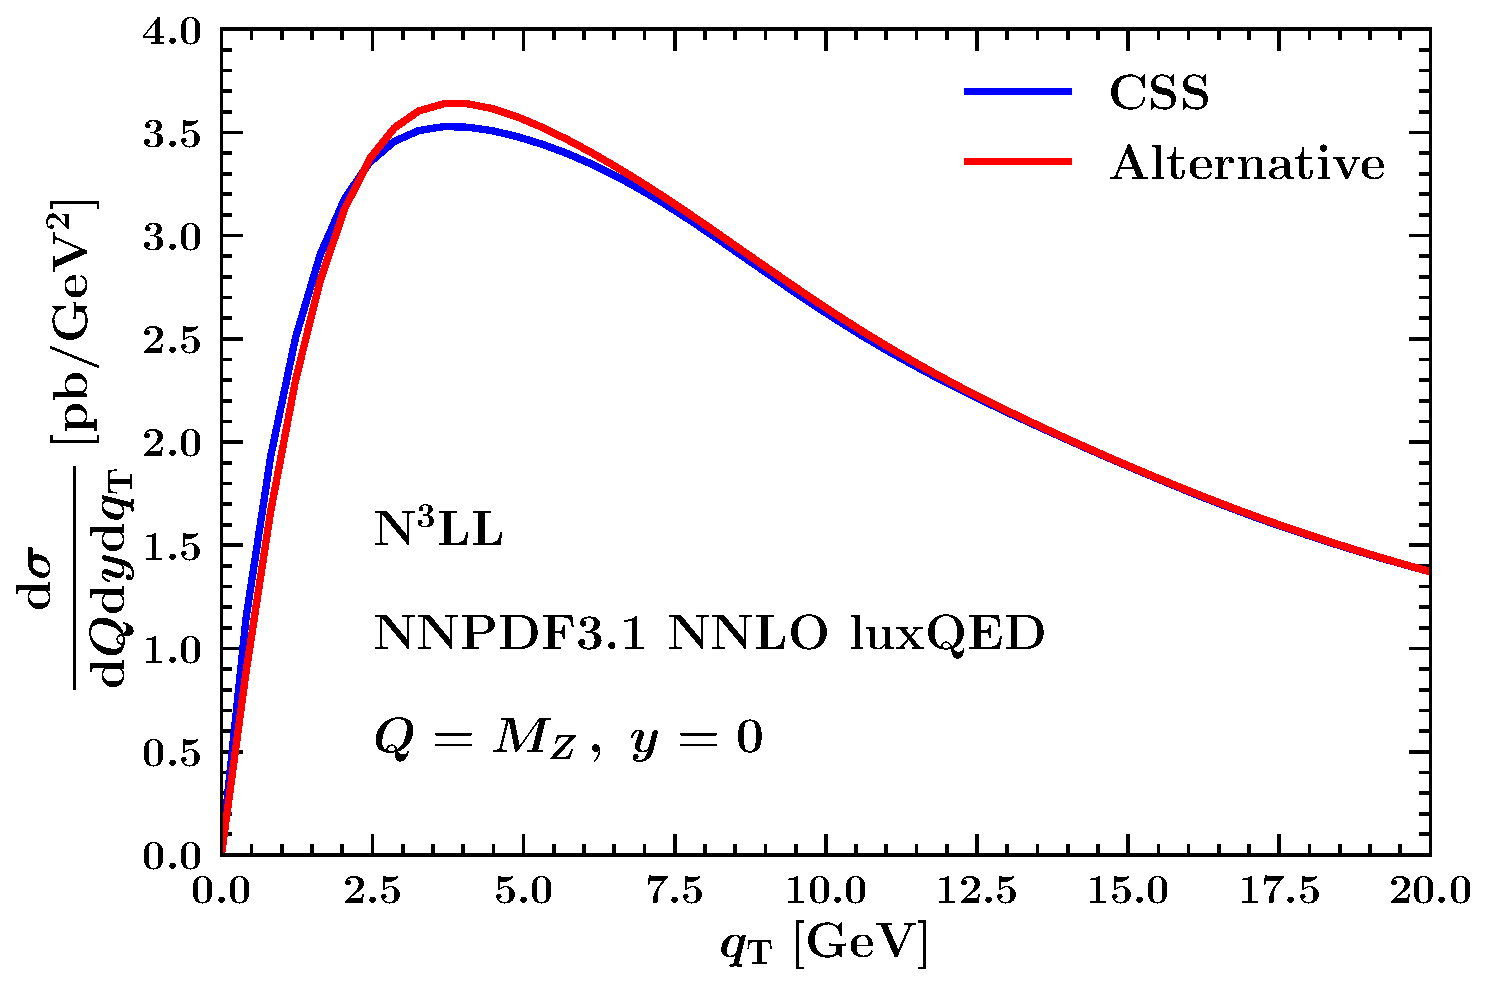
\includegraphics[width=0.6\textwidth]{plots/NewPrescription_qT.pdf}
    \caption{.\label{fig:NewPrescription_qT}}
  \end{centering}
\end{figure}

\section{Extraction of the singular behaviour for $q_T\rightarrow 0$}

In this section we derive the expansion of the different ingredients
of TMDs in order to finally extract the singular behaviour of a cross
section involving TMDs for $q_T\rightarrow 0$. This will eventually
serve to match the low-$q_T$ resummed calculation to the fixed-order
one valid at $q_T\simeq Q$.

\subsection{Expansion of the evolution kernel}

In this subsection, we work out the perturbative expansion of the
evolution kernel $R$ up to $\mathcal{O}(\alpha_s^2)$. This expansion
is useful to extract the (singular) asymptotic behaviour of a cross
section computed at fixed order in pQCD as $q_T$ tends to zero. Since
TMDs always appear in pairs in the computation of a cross section and
that the evolution kernel is universal, it is convenient to compute
the expansion of $R^2$. To do so, we start from
Eq.~(\ref{eq:evkernelexp}) where we set
$\mu_0=\sqrt{\zeta_0}=\mu_b=2e^{-\gamma_E}/{b_T}$ and
$\mu=\sqrt{\zeta}=Q$, possible scale variations can be reinstated at a
later stage:
\begin{equation}
  R^2 = \exp\left\{ K(\mu_b)\ln\frac{Q^2}{\mu_b^2}+\int_{\mu_b^2}^{Q^2}\frac{d\mu'^2}{\mu'^2}\left[\gamma_F(\alpha_s(\mu')) - \frac12\gamma_K(\alpha_s(\mu'))\ln\frac{Q^2}{\mu'^2}\right]\right\}\,.
\end{equation}
Now we use the expansions in Eqs.~(\ref{eq:GKexp}), (\ref{eq:Kexp})
and~(\ref{eq:GFexp}):
\begin{equation}
  R^2 = \exp\left\{\sum_{n=0}^\infty
    a_s^{n+1}(\mu_b)K^{(n,0)}\ln\frac{Q^2}{\mu_b^2}+\int_{\mu_b^2}^{Q^2}\frac{d\mu'^2}{\mu'^2}a_s^{n+1}(\mu')\left(\gamma_F^{(n)}
      - \frac12\gamma_K^{(n)}\ln\frac{Q^2}{\mu'^2}\right)\right\}\,,
\label{eq:Sudexp}
\end{equation}
where we have defined:
\begin{equation}
a_s = \frac{\alpha_s}{4\pi}\,.
\end{equation}
In order to carry out the perturbative expansion we need to write the
argument of the exponential in terms of a common value of $\alpha_s$
computed at some hard scale: the natural choice in view of the
matching is $\alpha_s(Q)$. This can be achieved by using the RGE for
$a_s$ at leading order:
\begin{equation}
\mu^2\frac{da_s}{d\mu^2}=-\beta_0a_s^2(\mu)\,,
\label{eq:RGEas}
\end{equation}
whose solution is:
\begin{equation}
a_s(\mu) = \frac{a_s(Q)}{1+a_s(Q)\beta_0\ln(\mu^2/Q^2)}\simeq
a_s(Q)\left[1+a_s(Q)\beta_0\ln(Q^2/\mu^2)+\mathcal{O}(a_s^2)\right]\,.
\label{eq:asexp}
\end{equation}
Plugging the expansion in the r.h.s. of Eq.~(\ref{eq:asexp}) into
Eq.~(\ref{eq:Sudexp}) and retaining only terms up to
$\mathcal{O}(a_s^2)$, one finds: 
\begin{equation}
\begin{array}{rcl}
  R^2 &=&\displaystyle \exp\Bigg\{ a_s(Q)\left[
          K^{(0,0)}\ln\frac{Q^2}{\mu_b^2}+\int_{\mu_b^2}^{Q^2}\frac{d\mu'^2}{\mu'^2}\left(\gamma_F^{(0)}
          - \frac12\gamma_K^{(0)}\ln\frac{Q^2}{\mu'^2}\right)\right]\\
\\
&+& \displaystyle a_s^2(Q)\beta_0\left[K^{(0,0)}\ln^2\frac{Q^2}{\mu_b^2}+\int_{\mu_b^2}^{Q^2}\frac{d\mu'^2}{\mu'^2}\left(\gamma_F^{(0)}\ln\frac{Q^2}{\mu'^2}
          - \frac12\gamma_K^{(0)}\ln^2\frac{Q^2}{\mu'^2}\right)\right]\\
\\
&+&\displaystyle a_s^2(Q)\left[K^{(1,0)}\ln\frac{Q^2}{\mu_b^2}+\int_{\mu_b^2}^{Q^2}\frac{d\mu'^2}{\mu'^2}\left(\gamma_F^{(1)}
          - \frac12\gamma_K^{(1)}\ln\frac{Q^2}{\mu'^2}\right)\right]+\mathcal{O}(a_s^3)\Bigg\}\,.
\end{array}
\label{eq:SudExp1}
\end{equation}
The final step before carrying out the expansion is computing the
integrals:
\begin{equation}
\int_{\mu_b^2}^{Q^2}\frac{d\mu'^2}{\mu'^2}\ln^k\left(\frac{Q^2}{\mu'^2}\right)
= \int_{\ln(\mu_b^2)}^{\ln
  Q^2}d\ln\mu'^2\ln^k\left(\frac{Q^2}{\mu'^2}\right) = \int^{\ln(Q^2/\mu_b^2)}_{0}dx\,x^k=\frac{1}{k+1}\ln^{k+1}\left(\frac{Q^2}{\mu_b^2}\right)\,.
\end{equation}
so that:
\begin{equation}
\begin{array}{rcl}
  R^2 &\simeq&\displaystyle \exp\Bigg\{ a_s(Q)\left[
          \left(K^{(0,0)}+\gamma_F^{(0)}\right)L - \frac14\gamma_K^{(0)}L^2
          \right]\\
\\
&+& \displaystyle a_s^2(Q)\bigg[\left(K^{(1,0)}+\gamma_F^{(1)}\right)L +\left(\beta_0 K^{(0,0)}+\frac12\beta_0\gamma_F^{(0)} - \frac14\gamma_K^{(1)}\right)L^2- \frac16 \beta_0\gamma_K^{(0)}L^3\bigg]\Bigg\}\,,
\end{array}
\label{eq:SudExp0}
\end{equation}
where we have defined:
%If we define:
\begin{equation}
L\equiv \ln\frac{Q^2}{\mu_b^2}\,,
\label{eq:reslogs}
\end{equation}
Eq.~(\ref{eq:SudExp1}) can be conveniently written as:
\begin{equation}
  R^2=\exp\left\{\sum_{n=1}^2a_s^n(Q)\sum_{k=1}^{n+1}S^{(n,k)}L^k\right\}\,,
\label{eq:SudCompact}
\end{equation}
with:
\begin{equation}
\begin{array}{l}
\displaystyle \displaystyle S^{(1,1)} =K^{(0,0)}+\gamma_F^{(0)}\,,\quad\displaystyle
                                                   S^{(1,2)} =- \frac14\gamma_K^{(0)}\,,\\
\\
\displaystyle S^{(2,1)} =K^{(1,0)}+\gamma_F^{(1)}\,,\quad\displaystyle S^{(2,2)} = \beta_0 K^{(0,0)}+\frac12\beta_0\gamma_F^{(0)} - \frac14\gamma_K^{(1)}\,,\quad\displaystyle S^{(2,3)} = - \frac16 \beta_0\gamma_K^{(0)}\,.
\end{array}
\end{equation}
Eq.~(\ref{eq:SudCompact}) can be easily expanded up to order $a_s^2$
as:
\begin{equation}
\begin{array}{rcl}
  \displaystyle R^2&=&\displaystyle
                       1+a_s(Q)\sum_{k=1}^{2}S^{(1,k)}L^k+a_s^2(Q)\left[\sum_{k=1}^{3}S^{(2,k)}L^k+\frac12\left(\sum_{k=1}^{2}S^{(1,k)}L^k\right)^2\right]+\mathcal{O}(a_s^3)\\
  \\
                   &=&\displaystyle
                       1+a_s(Q)\sum_{k=1}^{2}S^{(1,k)}L^k+a_s^2(Q)
                       \sum_{k=1}^{4}\widetilde{S}^{(2,k)}L^k
                       +\mathcal{O}(a_s^3)\,,
\end{array}
\label{eq:exp1}
\end{equation}
with:
\begin{equation}
\begin{array}{ll}
\displaystyle    \widetilde{S}^{(2,1)}={S}^{(2,1)}\,,&\displaystyle \quad \widetilde{S}^{(2,2)}={S}^{(2,2)}+\frac12\left[S^{(1,1)}\right]^2\,,\\
\\
\displaystyle
  \widetilde{S}^{(2,3)}={S}^{(2,3)}+{S}^{(1,1)}{S}^{(1,2)}\,,&\displaystyle
                                                                \quad \widetilde{S}^{(2,4)}=\frac12\left[S^{(1,2)}\right]^2\,.
\end{array}
\end{equation}

\subsection{Expansion of the DGLAP evolution}\label{eq:dglapexp}

A further step towards the extraction of the singular behaviour of the
resummed cross section in the limit $q_T\rightarrow 0$ requires
expanding the solution of the DGLAP equation that also resums
logarithms as that in Eq.~(\ref{eq:reslogs}). The solution of the
DGLAP equation in Eq.~(\ref{eq:DGLAPeq}) that evolves PDFs from the
scale $\mu_0=\mu_b$ to the scale $Q$ can be written as(\footnote{A
  summation over the flavour indices is understood}):
\begin{equation}
f(Q) = \Gamma(Q,\mu_b)\otimes f(\mu_b)\,,
\end{equation}
where the evolution operator $\Gamma$ obeys the equation:
\begin{equation}
\frac{\partial \Gamma(Q,\mu_b)}{\partial \ln Q^2} = P(Q) \otimes
\Gamma(Q,\mu_b)\,,
\label{eq:DGLAPeqOp}
\end{equation}
with the splitting functions $P$ having the perturbative expansion:
\begin{equation}
P(Q) =\sum_{n=0}^{\infty}a_s^{n+1}(Q) P^{(n)}\,.
\end{equation}
The coefficients $P^{(n)}$ are functions of $x$ (or $z$) only and thus
(in $\overline{\mbox{MS}}$) $P$ depends on $Q$ only through the
coupling $a_s$. We now need to expand $\Gamma$ in powers of $a_s$ up
to $\mathcal{O}(a_s^2)$. To this end, we assume that $\Gamma$ obeys
the expansion:
\begin{equation}
\Gamma(Q,\mu_b) = \Delta + \sum_{n=1}^{\infty} a_s^{n}(Q)\sum_{k=1}^{n}L^k\Gamma^{(n,k)}\,,
\end{equation}
where the coefficients $\Gamma^{(n,k)}$ are functions of $x$ only that
we need to determine up to $n=2$. Eq.~(\ref{eq:DGLAPeqOp}) can be
solved iteratively. At $\mathcal{O}(a_s)$, considering that:
\begin{equation}
\frac{da_s}{d \ln Q^2}=\mathcal{O}(a_s^2)\,,
\end{equation}
this gives:
\begin{equation}
\Gamma^{(1,1)}=P^{(0)}\,.
\end{equation}
At $\mathcal{O}(a_s^2)$, this gives:
\begin{equation}
-L\beta_0 P^{(0)} +\Gamma^{(2,1)}+2L\Gamma^{(2,2)}= P^{(1)}+L
P^{(0)}\otimes P^{(0)}\,,
\end{equation}
so that:
\begin{equation}
\begin{array}{l}
\displaystyle \Gamma^{(2,1)} = P^{(1)}\,,\\
\\
\displaystyle \Gamma^{(2,2)} = \frac12\beta_0 P^{(0)} + \frac12 P^{(0)}\otimes P^{(0)}\,.
\end{array}
\end{equation}
Putting all pieces together, we find:
\begin{equation}
\Gamma(Q,\mu_b) = \Delta + a_s(Q)L P^{(0)}
+a_s^2(Q)\left[LP^{(1)}+ \frac{L^2}2 \left(\beta_0 P^{(0)}
    +P^{(0)}\otimes P^{(0)}\right)\right]+\mathcal{O}(a_s^3)\,.
\label{eq:DGLAPeqOpExp}
\end{equation}
However, the quantity we are interested in is the inverse of the
operator $\Gamma$, that evolves the PDFs from the scale $Q$ to
$\mu_b$:
\begin{equation}
\begin{array}{l}
\displaystyle \Gamma(\mu_b,Q)=\Gamma^{-1}(Q,\mu_b) \\
\\\displaystyle
 = \Delta - a_s(Q)L P^{(0)}
- a_s^2(Q)\left[LP^{(1)}+ \frac{L^2}2 \left(\beta_0 P^{(0)}-P^{(0)}\otimes P^{(0)}\right)\right]+\mathcal{O}(a_s^3)\,.
\end{array}
\label{eq:DGLAPeqOp1}
\end{equation}

\subsection{Expansion of the matching coefficients at the hard scale}

The final step is the expansion of the matching coefficients $C$
defined in Eq.~(\ref{eq:matching}) for $\mu_0=\mu_b$ around the scale
$Q$ up to order $a_s^2$. To do this, we use the expansion in
Eq.~(\ref{eq:MatchCoeffExp}), in which $a_s$ is computed at $\mu_b$,
and combine it with Eq.~(\ref{eq:asexp}). This yields:
\begin{equation}
  C(\mu_b,\mu_b^2) = \Delta + a_s(Q) C^{(1,0)} + a_s^2(Q)
  \left[C^{(2,0)}+L\beta_0C^{(1,0)}\right]+\mathcal{O}(a_s^3)\,.
\label{eq:MatchCoeffExp1}
\end{equation}

\subsection{Expansion of the single low-scale TMD}

Before going into the more convoluted (but more relevant) case of a
cross section, it is useful to compute the expansion of a single
low-scale TMD, \textit{i.e.} the convolution between matching
coefficients and collinear distributions at the scale
$\mu_0=\mu_b$. This can be achieved combining
Eqs.~(\ref{eq:DGLAPeqOp1}) and~(\ref{eq:MatchCoeffExp1}):
\begin{equation}
\begin{array}{rcl}
C(\mu_b,\mu_b^2)\otimes f(\mu_b) &=& C(\mu_b,\mu_b^2)\otimes
\Gamma(\mu_b,Q) \otimes f(Q)\\
\\
&=& \bigg\{\Delta + a_s(Q)\left[C^{(1,0)}-L P^{(0)}\right]\\
\\
&+&\displaystyle a_s^2(Q)\bigg[C^{(2,0)}+L\left(-P^{(1)}-C^{(1,0)}\otimes P^{(0)}+\beta_0C^{(1,0)}\right)\\
\\
&+&\displaystyle \frac{L^2}2 \left(P^{(0)}\otimes P^{(0)}-\beta_0 P^{(0)}\right)\bigg]\bigg\}\otimes f(Q)+\mathcal{O}(a_s^3)\,.
\end{array}
\label{eq:LowScaleTMD}
\end{equation}

\subsection{Expansion of the cross section}

We are finally in the position to gather all pieces and write down the
perturbative expansion of a cross section involving TMDs, relevant in
the limit $q_T\rightarrow 0$. The only additional information required
is the hard factor $H$ that also admits a perturbative expansion. It
is now opportune to reinstate the flavour indices. In general, the
hard factor $H$ has a flavour structure, meaning that it carries a
pair of flavour indices. Choosing $\mu = Q$, the expansion of the hard
factor reads:
\begin{equation}
H_{ij}(Q) = \sum_{n=0}^\infty a_s^n(Q)
H_{ij}^{(n)}=H_{ij}^{(0)}+a_s(Q) H_{ij}^{(1)}+a_s^2(Q)
H_{ij}^{(2)}+\mathcal{O}(a_s^3)\,,
\label{eq:HardFactExp}
\end{equation}
where $H_{ij}^{(n)}$ are numerical factors. In relevant processes,
such as Drell-Yan and SIDIS, it turns out that up to
$\mathcal{O}(\alpha_s^2)$ the coefficients of the expansion of hard
factor $H$ are diagonal in flavour. Specifically, for scales
sufficiently below the $Z$-mass scale, we have:
\begin{equation}
H_{ij}^{(n)}\propto e_i^2\delta_{ij}\,,\quad\mbox{for}\quad n=0,1,2\,,
\end{equation}
where $e_i$ is the electric charge of the $i$-th quark flavour. For
higher scales, one just needs to replace the electric charges with the
effective electro-weak charges. This simplification does not hold
beyond $\mathcal{O}(\alpha_s^2)$.

A physical cross section differential in $q_T$ can finally be computed
as:
\begin{equation}
  \displaystyle \frac{d\sigma}{dq_T^2} \propto \sum_{ij}H_{ij} (Q)
  \int d^2\mathbf{b}_T e^{i \mathbf{b}_T\cdot \mathbf{q}_T}F_i(x,
  \mathbf{b}_T,Q,Q^2) D_j(z, \mathbf{b}_T,Q,Q^2)
\label{eq:qTspectrum}
\end{equation}
where $F_i$ and $D_j$ are two different sets of TMD distributions
(\textit{e.g.} a set of PDFs and a set of FFs) indexed by a flavour
index. Assuming that the flavour indices $i$ and $j$ run
\textit{either} on quarks \textit{or} on the gluon and writing
explicitly all perturbative factors, one has:
\begin{equation}
\begin{array}{rcl}
\displaystyle \frac{d\sigma}{dq_T^2} &\propto&\displaystyle  \sum_{ij}H_{ij} (Q) \int \frac{d^2\mathbf{b}_T}{4\pi} e^{i \mathbf{b}_T\cdot
  \mathbf{q}_T} R^2\left[(\mu_b,\mu_b^2)\rightarrow
  (Q,Q^2)\right] \\
\\
&\times&\displaystyle \sum_{k}\left[ \mathcal{C}_{ik}(x;\mu_b,\mu_b^2)\otimes
  f_k(x,\mu_b)\right]\sum_{l}\left[
  \mathbb{C}_{jl}(z;\mu_b,\mu_b^2)\otimes
  d_l(z,\mu_b)\right]\\
\\
&=&\displaystyle \sum_{n=0}^\infty a_s^n(Q)\sum_{p=0}^{2n} I_p(q_T,Q)
    \sum_{ij,kl} B_{ij,kl}^{(n,p)}(x,z) \mathop{\otimes}_x f_k(x,Q) \mathop{\otimes}_z d_l(z,Q)\,.
\end{array}
\label{eq:xsecexp}
\end{equation}
In the equation above we used different symbols to distinguish the
perturbative components of the distributions $F$ and $D$ because in
general they are different. In addition, we have defined:
\begin{equation}
I_p(q_T,Q)\equiv \int \frac{d^2\mathbf{b}_T}{4\pi} e^{i \mathbf{b}_T\cdot
  \mathbf{q}_T} \ln^p\left(\frac{b_T^2Q^2}{4e^{-2\gamma_E}}\right) =
\frac12\int_0^\infty db_T\,b_T J_0(b_Tq_T)
\ln^p\left(\frac{b_T^2Q^2}{4e^{-2\gamma_E}}\right)\,.
\label{eq:IkPert}
\end{equation}
Results for $I_p$ have been computed up to $p=4$ in Eq.~(136) of
Appendix B of Ref.~\cite{Bozzi:2005wk}. Specifically, and including
the trivial tranform with $p=0$, they read:
\begin{equation}
\begin{array}{l}
\displaystyle I_0(q_T,Q) = \delta(q_T^2)\,,\\
\\
\displaystyle I_1(q_T,Q) = - \frac{1}{q_T^2}\,,\\
\\
\displaystyle I_2(q_T,Q) = - \frac{2}{q_T^2}\ln\left(\frac{Q^2}{q_T^2}\right) \,,\\
\\
\displaystyle I_3(q_T,Q) = - \frac{3}{q_T^2}\ln^2\left(\frac{Q^2}{q_T^2}\right) \,,\\
\\
\displaystyle I_4(q_T,Q) = - \frac{4}{q_T^2}\left[\ln^3\left(\frac{Q^2}{q_T^2}\right)-4\zeta_3\right]\,.
\end{array}
\label{eq:PureLogs}
\end{equation}
The functions above are compute under the assumption that there is no
non-perturbative component. Upon this assumption, that we will relax
below, all terms with $p=0$ will be proportional to
$\delta(q_T^2)$. Analogous terms are \textit{not} included in the
fixed-order calculation. Therefore, when matching the resummed
calculation to the fixed-order one, one should remove from
Eq.~(\ref{eq:xsecexp}) all terms with $p=0$. Importantly, this means
removing the full $\mathcal{O}(1)$ terms such that the leading-order
term for $q_T>0$ is $\mathcal{O}(a_s)$.

The coefficients $B^{(n,k)}$ in Eq.~(\ref{eq:xsecexp}) can be
determined by using the expansions worked out above in
Eqs.~(\ref{eq:exp1}), (\ref{eq:LowScaleTMD}),
and~(\ref{eq:HardFactExp}). The leading order is obtained by just
retaining the $\mathcal{O}(a_s^0)$ terms in all the expansions. This
gives:
\begin{equation}
B_{ij,kl}^{(0,0)}(x,z) =
H_{ij}^{(0)}\delta_{ik}\delta_{jl}\delta(1-x)\delta(1-z)\,.
\label{eq:BLO}
\end{equation}

The $\mathcal{O}(a_s)$ terms are obtained by combining the
leading-order ones of all expansions but one. Finally organising the
terms in powers of $L$, this yields:
\begin{equation}
\begin{array}{rcl}
B_{ij,kl}^{(1,0)}(x,z) &=& \displaystyle H_{ij}^{(1)}\delta_{ik}\delta(1-x) \delta_{jl}\delta(1-z)+H_{ij}^{(0)}\delta_{ik}\delta(1-x)\mathbb{C}_{jl}^{(1,0)}(z)+H_{ij}^{(0)}\mathcal{C}_{ik}^{(1,0)}(x)\delta_{jl}\delta(1-z)\,,\\
\\
B_{ij,kl}^{(1,1)}(x,z) &=& \displaystyle H_{ij}^{(0)} S^{(1,1)}\delta_{ik}\delta(1-x) \delta_{jl}\delta(1-z)-H_{ij}^{(0)}\delta_{ik}\delta(1-x)\mathbb{P}_{jl}^{(0)}(z)-H_{ij}^{(0)}\mathcal{P}_{ik}^{(0)}(x)\delta_{jl}\delta(1-z)\,,\\
\\
B_{ij,kl}^{(1,2)}(x,z) &=& \displaystyle H_{ij}^{(0)} S^{(1,2)}\delta_{ik}\delta(1-x) \delta_{jl}\delta(1-z)\,.
\end{array}
\label{eq:BNLO}
\end{equation}

Finally, the $\mathcal{O}(a_s^2)$ terms are more convoluted and read:
\begin{equation}
\begin{array}{rcl}
  {B}_{ij,kl}^{(2,0)}(x,z) &=&\displaystyle H_{ij}^{(2)}
                               \delta_{ik}\delta(1-x) \delta_{jl}\delta(1-z) \,,\\
  \\
                           &+&\displaystyle
                               H_{ij}^{(1)}\left[\mathcal{C}_{ik}^{(1,0)}(x)\delta_{jl}\delta(1-z)
                               +
                               \delta_{ik}\delta(1-x)\mathbb{C}_{jl}^{(1,0)}(z)\right]\\
  \\
                           &+&\displaystyle H_{ij}^{(0)}\mathcal{C}_{ik}^{(2,0)}(x)\delta_{jl}\delta(1-z) + 
                               H_{ij}^{(0)}\mathcal{C}_{ik}^{(1,0)}(x)\mathbb{C}_{jl}^{(1,0)}(z)
                               +H_{ij}^{(0)}\delta_{ik}\delta(1-x)\mathbb{C}_{jl}^{(2,0)}(z)\,,\\
  \\
  {B}_{ij,kl}^{(2,1)}(x,z) &=&\displaystyle \left(H_{ij}^{(0)}\widetilde{S}^{(2,1)}+H_{ij}^{(1)}S^{(1,1)}\right)
                              \delta_{ik}\delta(1-x) \delta_{jl}\delta(1-z)\\
  \\
                          &-& \displaystyle
                              H_{ij}^{(1)}\left[\mathcal{P}_{ik}^{(0)}(x)\delta_{jl}\delta(1-z)
                              +
                              \delta_{ik}\delta(1-x)\mathbb{P}_{jl}^{(0)}(z)\right]\\
  \\
                          &+&
                              H_{ij}^{(0)} S^{(1,1)}\left[\mathcal{C}_{ik}^{(1,0)}(x)\delta_{jl}\delta(1-z)
                              +
                              \delta_{ik}\delta(1-x)\mathbb{C}_{jl}^{(1,0)}(z)\right]\\
  \\
                          &+&\displaystyle 
                              H_{ij}^{(0)}\left(-\mathcal{P}^{(1)}(x)-\sum_\alpha
                              \mathcal{C}_{i\alpha}^{(1,0)}(x)\otimes
                              \mathcal{P}_{\alpha k}^{(0)}(x)+\beta_0\mathcal{C}_{ik}^{(1,0)}(x)\right)\delta_{jl}\delta(1-z)\\
\\
 &-&\displaystyle H_{ij}^{(0)}\mathcal{P}_{ik}^{(0)}(x)\mathbb{C}_{jl}^{(1,0)}(z)
     -H_{ij}^{(0)}\mathcal{C}_{ik}^{(1,0)}(x)\mathbb{P}_{jl}^{(0)}(z)\\
\\
                              &+&\displaystyle H_{ij}^{(0)}\delta_{jl}\delta(1-z) \left(-\mathbb{P}^{(1)}(z)-\sum_\beta
                              \mathbb{C}_{j\beta}^{(1,0)}(z)\otimes
                              \mathbb{P}_{\beta l}^{(0)}(z)+\beta_0\mathbb{C}_{jl}^{(1,0)}(z)\right) \,,\\
  \\
  {B}_{ij,kl}^{(2,2)}(x,z) &=&\displaystyle \left( H_{ij}^{(0)}\widetilde{S}^{(2,2)}+H_{ij}^{(1)}S^{(1,2)}\right)
                              \delta_{ik}\delta(1-x) \delta_{jl}\delta(1-z)\\
  \\
                          &+&\displaystyle
                              H_{ij}^{(0)}{S}^{(1,2)}\left[\mathcal{C}_{ik}^{(1,0)}(x)\delta_{jl}\delta(1-z)+\delta_{ik}\delta(1-x)\mathbb{C}_{jl}^{(1,0)}(z)\right]\\
  \\
                          &-&\displaystyle
                              H_{ij}^{(0)} S^{(1,1)}\left[\mathcal{P}_{ik}^{(0)}(x)\delta_{jl}\delta(1-z)+\delta_{ik}\delta(1-x)\mathbb{P}_{jl}^{(0)}(z)\right]\\
  \\
 &+& \displaystyle
     H_{ij}^{(0)}\mathcal{P}_{ik}^{(0)}(x)\mathbb{P}_{jl}^{(0)}(z)\\
\\
                          &+& \displaystyle H_{ij}^{(0)}\frac12\left(\sum_{\alpha}\mathcal{P}^{(0)}_{i\alpha}(x)\otimes
    \mathcal{P}_{\alpha k}^{(0)}(x)-\beta_0 \mathcal{P}_{ik}^{(0)}(x)\right)\delta_{jl}\delta(1-z)\\
\\
                              &+&\displaystyle H_{ij}^{(0)}\delta_{ik}\delta(1-x) \frac12 \left(\sum_{\beta}\mathbb{P}^{(0)}_{j\beta}(z)\otimes
    \mathbb{P}_{\beta l}^{(0)}(z) -\beta_0 \mathbb{P}_{jl}^{(0)}(z)\right)\,,\\
  \\
  {B}_{ij,kl}^{(2,3)}(x,z) &=&\displaystyle
                              H_{ij}^{(0)}\widetilde{S}^{(2,3)}\delta_{ik}\delta(1-x) \delta_{jl}\delta(1-z)
                              - H_{ij}^{(0)} S^{(1,2)}\left[\mathcal{P}_{ik}^{(0)}(x)\delta_{jl}\delta(1-z)
                              +
                              \delta_{ik}\delta(1-x)\mathbb{P}_{jl}^{(0)}(z)\right]\,,\\
  \\
  {B}_{ij,kl}^{(2,4)}(x,z) &=&\displaystyle H_{ij}^{(0)}\widetilde{S}^{(2,4)}\delta_{ik}\delta(1-x) \delta_{jl}\delta(1-z) \,.
\end{array}
\label{eq:BNNLO}
\end{equation}

\subsection{Scale variations}

In this section, we work out the expressions for the renormalisation-
and factorisation-scale variations of the expanded cross section up to
$\mathcal{O}(\alpha_s^2)$. This is done by displacing the coupling
from $Q$ to $\mu_{\rm R}$ and the PDFs/FFs from $Q$ to $\mu_{\rm
  F}$. Under the assumption that
$\mu_{\rm R}\simeq \mu_{\rm R}\simeq Q$, this displacements can be
obtained by expanding the solutions of the evolution equation between
$Q$ and $\mu_{\rm R}$ or $\mu_{\rm F}$ up to
$\mathcal{O}(\alpha_s^2)$.  For the coupling, this expansion can be
read off from Eq.~(\ref{eq:alphasexp}):
\begin{equation}
\begin{array}{rcl}
a_s(Q) &=&\displaystyle a_s(\mu_{\rm R}) \bigg[ 1 + a_s(\mu_{\rm R})
           \beta_0  \ln\frac {\mu_{\rm R}^2}{Q^2}\bigg]
                                          +\mathcal{O}(\alpha_s^3)\,.
\end{array}
\label{eq:alphasexp2}
\end{equation}
For the PDFs/FFs, the expansion of the evolution operator can be read
off from Eq.~(\ref{eq:DGLAPeqOpExp}):
\begin{equation}
\Gamma(Q,\mu_{\rm F}) = \Delta - a_s(Q)\ln\frac {\mu_{\rm F}^2}{Q^2} P^{(0)}
-a_s^2(Q)\left[\ln\frac {\mu_{\rm F}^2}{Q^2} P^{(1)}- \frac{1}2 \ln^2\frac{\mu_{\rm F}^2}{Q^2} \left(\beta_0 P^{(0)} +P^{(0)}\otimes P^{(0)}\right)\right]+\mathcal{O}(\alpha_s^3)\,,
\end{equation}
with $\Delta_{ij}(x) = \delta_{ij}\delta(1-x)$. We now use
Eq.~(\ref{eq:alphasexp2}) to replace $a_s(Q)$ with $a_s(\mu_{\rm R})$
in the expression above and get:
\begin{equation}
\begin{array}{rcl}
\Gamma(Q,\mu_{\rm F}) &=&\displaystyle  \Delta -a_s(\mu_{\rm R})
                          \ln\frac {\mu_{\rm F}^2}{Q^2} P^{(0)}\\
\\
&-&\displaystyle a_s^2(\mu_{\rm R})\left[\ln\frac {\mu_{\rm F}^2}{Q^2} P^{(1)}
                          +\left(\ln\frac {\mu_{\rm R}^2}{Q^2} -\frac{1}2 \ln\frac{\mu_{\rm F}^2}{Q^2}\right) \ln\frac {\mu_{\rm F}^2}{Q^2}\beta_0 P^{(0)} -\frac{1}2 \ln^2\frac{\mu_{\rm F}^2}{Q^2} P^{(0)}\otimes
                          P^{(0)} \right]+\mathcal{O}(\alpha_s^3)\,.
\end{array}
\label{eq:PDFFFEvExp}
\end{equation}
Since we have two such operators, one for the PDFs and one for the
FFs, it is convenient to take the product beforehand and truncate it
to $\mathcal{O}(\alpha_s^2)$ so that:
\begin{equation}
\begin{array}{rcl}
f_k(x,Q) d_l(z,Q) &=&\displaystyle
                      \Bigg[\delta_{km}\delta(1-x)\delta_{ln}\delta(1-z)\\
\\
 &-&\displaystyle a_s(\mu_{\rm R})
                          L_{\rm F} \left(\delta_{km}\delta(1-x)\mathbb{P}_{ln}^{(0)}(z)+\mathcal{P}_{km}^{(0)}(x)\delta_{ln}\delta(1-z)\right)\\
\\
&-&\displaystyle a_s^2(\mu_{\rm R})\bigg[L_{\rm F} \left(\delta_{km}\delta(1-x)\mathbb{P}_{ln}^{(1)}(z)+\mathcal{P}_{km}^{(1)}(x)\delta_{ln}\delta(1-z)\right)
                          \\
\\
&+&\displaystyle \left(L_{\rm R}
    -\frac{1}2 L_{\rm F}\right) L_{\rm F}\beta_0 \left(\delta_{km}\delta(1-x)\mathbb{P}_{ln}^{(0)}(z)+\mathcal{P}_{km}^{(0)}(x)\delta_{ln}\delta(1-z)\right)
  \\
\\
&-&\displaystyle \frac{1}2 L_{\rm F}^2\left(\delta_{km}\delta(1-x)\mathbb{P}_{l\beta}^{(0)}(z)\otimes
                          \mathbb{P}_{\beta n}^{(0)}(z) +2 \mathcal{P}_{km}^{(0)}(x) \mathbb{P}_{ln}^{(0)}(z)+\mathcal{P}_{k\beta}^{(0)}(x)\otimes
                          \mathcal{P}_{\beta m}^{(0)}(x) \delta_{ln}\delta(1-z)\right)\bigg]\\
\\
&&\displaystyle \Bigg]\mathop{\otimes}_x
    f_m(x,\mu_{\rm F}) \mathop{\otimes}_z
    d_n(z,\mu_{\rm F})\,,
\end{array}
\label{eq:expPDFsFFs}
\end{equation}
where the greek indices are undestood to be summed over and where we
have defined:
\begin{equation}
L_{\rm R} = \ln\frac {\mu_{\rm R}^2}{Q^2}\quad\mbox{and}\quad L_{\rm F} = \ln\frac {\mu_{\rm F}^2}{Q^2}\,.
\end{equation}
Finally, using Eqs.~(\ref{eq:alphasexp2}) and~(\ref{eq:expPDFsFFs})
the expansion of the cross section in Eq.~(\ref{eq:xsecexp}) can be
generalised to:
\begin{equation}
\begin{array}{rcl}
\displaystyle \frac{d\sigma}{dq_T^2} &\propto&\displaystyle
                                               \sum_{s=0}^\infty
                                               a_s^s(\mu_{\rm R})\sum_{p=0}^{2s} I_p(q_T,Q)
    \sum_{ij,kl} \overline{B}_{ij,mn}^{(s,p)}(x,z) \mathop{\otimes}_x f_m(x, \mu_{\rm F}) \mathop{\otimes}_z d_n(z, \mu_{\rm F})\,.
\end{array}
\end{equation}
where:
\begin{equation}
\begin{array}{rcl}
\overline{B}_{ij,mn}^{(0,0)}(x,z) &=&\displaystyle B_{ij,mn}^{(0,0)}(x,z)\,,\\
\\
\overline{B}_{ij,mn}^{(1,0)}(x,z) &=& \displaystyle B_{ij,mn}^{(1,0)}(x,z) - L_{\rm F} H_{ij}^{(0)}\left(\delta_{im}\delta(1-x) \mathbb{P}_{jn}^{(0)}(z)+\mathcal{P}_{im}^{(0)}(x) \delta_{jn}\delta(1-z)\right) \,,\\
\\
\overline{B}_{ij,mn}^{(1,1)}(x,z) &=& \displaystyle B_{ij,mn}^{(1,1)}(x,z) \,, \\
\\
\overline{B}_{ij,mn}^{(1,2)}(x,z) &=& \displaystyle B_{ij,mn}^{(1,2)}(x,z) \,, \\
\\
\overline{B}_{ij,mn}^{(2,0)}(x,z) &=&\displaystyle
                                      B_{ij,mn}^{(2,0)}(x,z) +
                                      \beta_0L_{\rm
                                      R}H_{ij}^{(0)}\left(\delta_{im}\delta(1-x)\mathbb{C}_{jn}^{(1,0)}(z)+\mathcal{C}_{im}^{(1,0)}(x)\delta_{jn}\delta(1-z)\right) \\
\\
&-&\displaystyle L_{\rm F}H_{ij}^{(0)}
    \bigg(\delta_{im}\delta(1-x)\mathbb{C}_{j\beta}^{(1,0)}(z) \mathop{\otimes}_z\mathbb{P}_{\beta n}^{(0)}(z)+\mathcal{C}_{im}^{(1,0)}(x)\mathbb{P}_{j n}^{(0)}(z)\\
\\
&+&\displaystyle \mathcal{P}_{i m}^{(0)}(x)\mathbb{C}_{jn}^{(1,0)}(z)+\mathcal{C}_{i\beta}^{(1,0)}(x) \mathop{\otimes}_x\mathcal{P}_{\beta m}^{(0)}(x)\delta_{jn}\delta(1-z)\bigg)\\
\\
&+&\displaystyle 
    H_{ij}^{(1)}\left(\beta_0L_{\rm R}\delta_{im}\delta(1-x) \delta_{jn}\delta(1-z)-L_{\rm F}\delta_{im}\delta(1-x)
    \mathbb{P}_{j n}^{(0)}(z) -L_{\rm F}
    \mathcal{P}_{i m}^{(0)}(x) \delta_{jn}\delta(1-z)\right)\\
\\
&-&\displaystyle  H_{ij}^{(0)}\bigg[L_{\rm F} \left(\delta_{im}\delta(1-x)\mathbb{P}_{jn}^{(1)}(z)+\mathcal{P}_{im}^{(1)}(x)\delta_{jn}\delta(1-z)\right)
                          \\
\\
&+&\displaystyle \left(L_{\rm R}
    -\frac{1}2 L_{\rm F}\right) L_{\rm F}\beta_0 \left(\delta_{im}\delta(1-x)\mathbb{P}_{jn}^{(0)}(z)+\mathcal{P}_{im}^{(0)}(x)\delta_{ln}\delta(1-z)\right)
  \\
\\
&-&\displaystyle \frac{1}2 L_{\rm F}^2\left(\delta_{im}\delta(1-x)\mathbb{P}_{j\beta}^{(0)}(z)\otimes
                          \mathbb{P}_{\beta n}^{(0)}(z) +2 \mathcal{P}_{im}^{(0)}(x) \mathbb{P}_{jn}^{(0)}(z)+\mathcal{P}_{i\beta}^{(0)}(x)\otimes
                          \mathcal{P}_{\beta m}^{(0)}(x) \delta_{jn}\delta(1-z)\right)\bigg]\,,\\
  \\
\overline{B}_{ij,mn}^{(2,1)}(x,z) &=&\displaystyle B_{ij,mn}^{(2,1)}(x,z) - \beta_0L_{\rm R}H_{ij}^{(0)}\left(\delta_{im}\delta(1-x)\mathbb{P}_{jn}^{(0)}(z)+\mathcal{P}_{im}^{(0)}(x)\delta_{jn}\delta(1-z)\right)\\
  \\
&+&\displaystyle L_{\rm F}
    H_{ij}^{(0)}\bigg(\delta_{im}\delta(1-x)\mathbb{P}_{j\beta}^{(0)}(z)
    \mathop{\otimes}_z\mathbb{P}_{\beta
    n}^{(0)}(z)+2\mathcal{P}_{im}^{(0)}(x)\mathbb{P}_{j n}^{(0)}(z)+\mathcal{P}_{i\beta}^{(0)}(x) \mathop{\otimes}_x\mathcal{P}_{\beta m}^{(0)}(x)\delta_{jn}\delta(1-z) \bigg)\\
\\
&+&\displaystyle 
    H_{ij}^{(0)} S^{(1,1)}\left(\beta_0L_{\rm R}\delta_{im}\delta(1-x) \delta_{jn}\delta(1-z)-L_{\rm F}\delta_{im}\delta(1-x)
    \mathbb{P}_{j n}^{(0)}(z) -L_{\rm F}
    \mathcal{P}_{i m}^{(0)}(x) \delta_{jn}\delta(1-z)\right) \,,\\
\\
\overline{B}_{ij,mn}^{(2,2)}(x,z) &=&\displaystyle B_{ij,mn}^{(2,2)}(x,z) \\
\\
&+&\displaystyle 
    H_{ij}^{(0)} S^{(1,2)}\left(\beta_0L_{\rm R}\delta_{im}\delta(1-x) \delta_{jn}\delta(1-z)-L_{\rm F}\delta_{im}\delta(1-x)
    \mathbb{P}_{j n}^{(0)}(z) -L_{\rm F}
    \mathcal{P}_{i m}^{(0)}(x) \delta_{jn}\delta(1-z)\right) \,,\\
\\
\overline{B}_{ij,mn}^{(2,3)}(x,z) &=&\displaystyle B_{ij,mn}^{(2,3)}(x,z) \,, \\
\\
\overline{B}_{ij,mn}^{(2,4)}(x,z) &=&\displaystyle B_{ij,mn}^{(2,4)}(x,z) \,,
\end{array}
\end{equation}
with the coefficients $B_{ij,mn}^{(s,p)}$ given in
Eqs.~(\ref{eq:BLO}), ~(\ref{eq:BNLO}), and~(\ref{eq:BNNLO}). Of
course, if $\mu_{\rm R}=\mu_{\rm F}=Q$, all logs vanish and the
$\overline{B}_{ij,mn}^{(s,p)}$ coefficients automatically reduce to
$B_{ij,mn}^{(s,p)}$.

\subsection{A note on the logarithmic ordering}

The logarithmic accuracy is driven by the evolution kernel $R$ defined
in Eq.~(\ref{eq:evkernel}). As it should be clear from
Eq.~(\ref{eq:exp1}), the evolution kernel squared $R^2$, also referred
to as Sudakov form factor, admits the following expansion:
\begin{equation}
R^2 = \sum_{n=0}^\infty a_s^{n}\sum_{k=1}^{2n}\widetilde{S}^{(n,k)}L^k\,.
\end{equation}
This expansion naturally allows us to define a logarithmic ordering
such that:
\begin{equation}
R^2 = \sum_{m=0}^{\infty}  R_{\rm N^mLL}^2\,,
\end{equation}
with:
\begin{equation}
  R_{\rm N^mLL}^2 = \sum_{n=[m/2]}^\infty \widetilde{S}^{(n,2n-m)}\,a_s^{n}L^{2n-m}\,,
\end{equation}
where $[m/2]$ stands for ``integer part of $m/2$''. Now, I multiply
$R_{\rm N^mLL}^2$ by $a_s$ to a generic power $p$ and do some
manipulation defining $n+p=j$. This way, I get:
\begin{equation}
a_s^p R_{\rm N^mLL}^2 = \sum_{j=[(m+2p)/2]}^\infty
\widetilde{S}^{(j-p,2j-(m+2p))}\,a_s^{j}L^{2j-(m+2p)}\sim R_{\rm
  N^{m+2p}LL}^2\,,
\label{eq:LogAcc}
\end{equation}
where the symbol $\sim$ means that the terms at two sides have the
same logarithmic accuracy. This finding is relevant in that, in order
to compute a cross section, the Sudakov from factor has to be
multiplied by the hard factor $H$ and a pair of matching functions
$C$. Both these components admit an expansion in powers of $a_s$
without enhancing logaritms $L$ (see Eqs.~(\ref{eq:MatchCoeffExp})
and~(\ref{eq:HardFactExp})). Therefore $R^2$ will eventually be
multiplied by some power of $a_s$.

Suppose we compute the Sudakov form factor to leading-logarithmic (LL)
accuracy ($m=0$): Eq.~(\ref{eq:LogAcc}) tells us that, in terms of
logarithmic accuracy, including $\mathcal{O}(a_s)$ corrections in $H$
and $C$ implies introducing next-to-next-to-leading-logarithmic (NNLL)
corrections. In practice, this means that to LL and NLL the functions
$H$ and $C$ can be taken at leading order, at NNLL we only need to
introduce $\mathcal{O}(a_s)$ corrections in $H$ and $C$, while at
N$^3$LL we have to introduce $\mathcal{O}(a_s^2)$ corrections in $H$
and $C$.

% However, this counting causes some apparent difficulty when
% considering the matching of the resummed and fixed-order
% calculations. Suppose, one want to match the N$^r$LL resummed
% calculation to the N$^f$LO fixed-order calculation. In order to
% subtract the double counting in an additive fashion, one needs to
% expand the resummed cross section to
% $\mathcal{O}(a_s^{p_{\rm LO}+f})$, with $p_{\rm LO}$ the leading-order
% power in $a_s$ of the fixed-order cross section. Since, both $H$ and
% $C$ start at $\mathcal{O}(1)$, this means that it is necessary to know
% both these components to $\mathcal{O}(a_s^{p_{\rm LO}+f})$. Since for
% Drell-Yan $p_{\rm LO} = 1$ and we currently know $C$ up to
% $\mathcal{O}(a_s^2)$, the highest order we can consider for the
% fixed-order calculation in next-to-leading order ($f=1$). In other
% words, the best we can do employing an additive matching seems to be
% N$^3$LL + NLO.

As a final remark, we notice that, as opposed to the Sudakov form
factor, the evolution of collinear distributions and $\alpha_s$
provide resummation of single logarithms. Therefore, the inclusion of
perturbative corrections to the $\beta$-functions and splitting
functions should be accordingly. Specifically, the perturbative
accuracy at which they are computed should be the same as that of the
non-cusp anomalous dimension $\gamma_F$.

\section{Non-perturbative effect on the asymptotic cross section}

As discussed in Sect.~\ref{sec:nonpert}, TMDs have a non-perturbative
component that can be parameterised as in
Eq.~(\ref{eq:separatation}). This implies two main ingredients: the
introduction of a function $b_*(b_T)$ that prevents the perturbative
component to enter the non-perturbative regime and a function
$f_{\rm NP}$ that parametrises the actual non-perturbative
component. These changes leave almost unchanged the derivation of the
asymptotic behavior of a cross section for $q_T\rightarrow 0$. The
only change concerns the functions $I_p$ defined in
Eq.~(\ref{eq:IkPert}), that have to be replaced with:
\begin{equation}
  \widetilde{I}_p(x,z,q_T,Q)\equiv \frac12\int_0^\infty db_T\,b_T J_0(b_Tq_T) f_{\rm NP}^{(1)}(x,
  {b}_T,Q^2) f_{\rm NP}^{(2)}(z,
  {b}_T,Q^2)\ln^p\left(\frac{b_*^2(b_T)Q^2}{4e^{-2\gamma_E}}\right)\,,
\label{eq:IkNonPert}
\end{equation}
where $f_{\rm NP}^{(1)}$ and $f_{\rm NP}^{(2)}$ are the
non-perturbative functions associated to the two TMD distributions $F$
and $D$ involved in the cross sections. Here we are assuming
$\mu=\sqrt{\zeta}=Q$ and $\mu_0=\sqrt{\zeta_0}=\mu_b$. In general, the
integral in Eq.~(\ref{eq:IkNonPert}) cannot be evaluated analytically
but one can use the Ogata quadrature method to compute it
numerically.(\footnote{The convergence of the Ogata quadrature method
  crucially depends on the function $f_{\rm NP}$ being exponentially
  suppressed for large values of $b_T$, such that full integrand is
  dumped in this region.}) In the case $k=0$ Eq.~(\ref{eq:IkNonPert})
has an intersting consequence. Specifically, contrary to the case in
which no non-perturbative contribution is introduced,
$\widetilde{I}_0$ is different from zero also for $q_T>0$. Therefore,
also the terms in the expansion in Eq.~(\ref{eq:xsecexp}) that are
independent of $L$ contribute to the cross section differential in
$q_T$. Clearly, any non-perturbative contribution is expected to give
a substantial contribution only in the vicinity of $q_T=0$.

In this respect, one should check that the introduction of the
non-perturbative components does not affect the large-$q_T$
region. This is amounts to showing that:
\begin{equation}
\widetilde{I}_p(x,z,q_T,Q)\mathop{\sim}_{q_T\gtrsim Q} I_p(q_T,Q)\,.
\label{eq:LogAsympt}
\end{equation}
Since for small values of $b_T$ we (must) have that
$b_*(b_T)\simeq b_T$ and that $f_{\rm NP}(x,b_T,\zeta)\simeq 1$, this
implies that for large values of $q_T$ (that is the conjugate variable
of $b_T$) $\widetilde{I}_p$ has to tend to $I_p$. This can be shown
numerically on a case-by-case base. In particular, we can compute the
integral in Eq.~(\ref{eq:IkNonPert}) using the Ogata quadrature method
and compare the results to those in Eq.~(\ref{eq:PureLogs}). For the
comparison we use Eq.~(\ref{eq:bstardefCSS}) with
$b_{\rm max} = 2e^{-\gamma_E}$ and choose as a non-perturbative
functions $f_{\rm NP}$ the following $x$-independent form:
\begin{equation}
f_{\rm NP}^{(1)}({b}_T,\zeta) = f_{\rm NP}^{(2)}({b}_T,\zeta) = \exp\left[\left( - g_1 - g_2 \ln\left( \frac{\sqrt{\zeta}}{2 Q_0}\right) \right) \frac{b_T^2}{2}\right]\,,
\end{equation}
with $g_1 = 0.02$, $g_1=0.5$, and $Q_0 = 1.6$~GeV.
\begin{figure}[h]
  \begin{centering}
    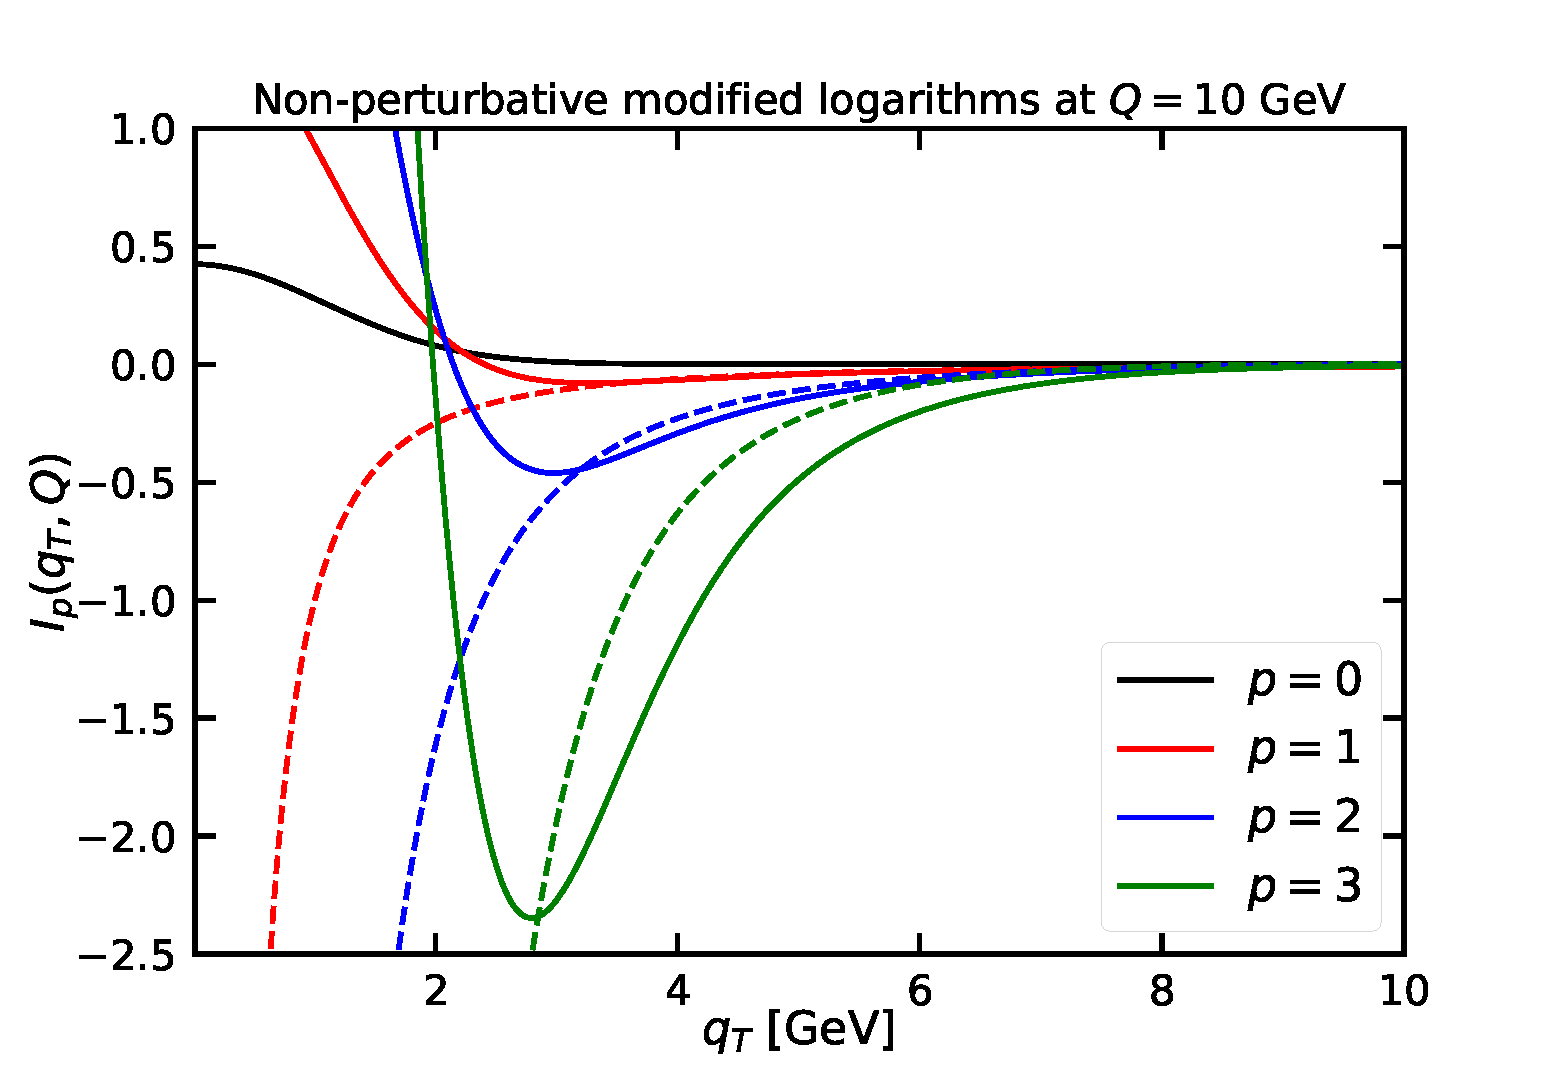
\includegraphics[width=0.45\textwidth]{plots/logs.pdf}
    \caption{Comparison of the integral in Eq.~(\ref{eq:IkNonPert})
      for $p=0,1,2,3$ (solid lines) to the expressions in
      Eq.~(\ref{eq:PureLogs}) (dashed lines) as functions of $q_T$ at
      $Q = 10$~GeV. The black dashed line is not present because it
      corresponds to $\delta(q_T^2)$.\label{fig:logs}}
  \end{centering}
\end{figure}

In Fig.~\ref{fig:logs}, I compare the integral in
Eq.~(\ref{eq:IkNonPert}) for $p=0,1,2,3$ (solid lines) to the
expressions in Eq.~(\ref{eq:PureLogs}) (dashed lines) at $Q = 10$~GeV
as functions of $q_T$. Notice that the black dashed line is not
present because it corresponds to $\delta(q_T^2)$. It is thus true
that $\widetilde{I}_p$ tends to $I_p$ as $q_T$ increases. However,
this is not enough to satisfy Eq.~(\ref{eq:LogAsympt}). As a matter of
fact, if one zooms in around $q_T\lesssim Q$, one finds a substantial
difference between $\widetilde{I}_p$ and $I_p$.
\begin{figure}[h]
  \begin{centering}
    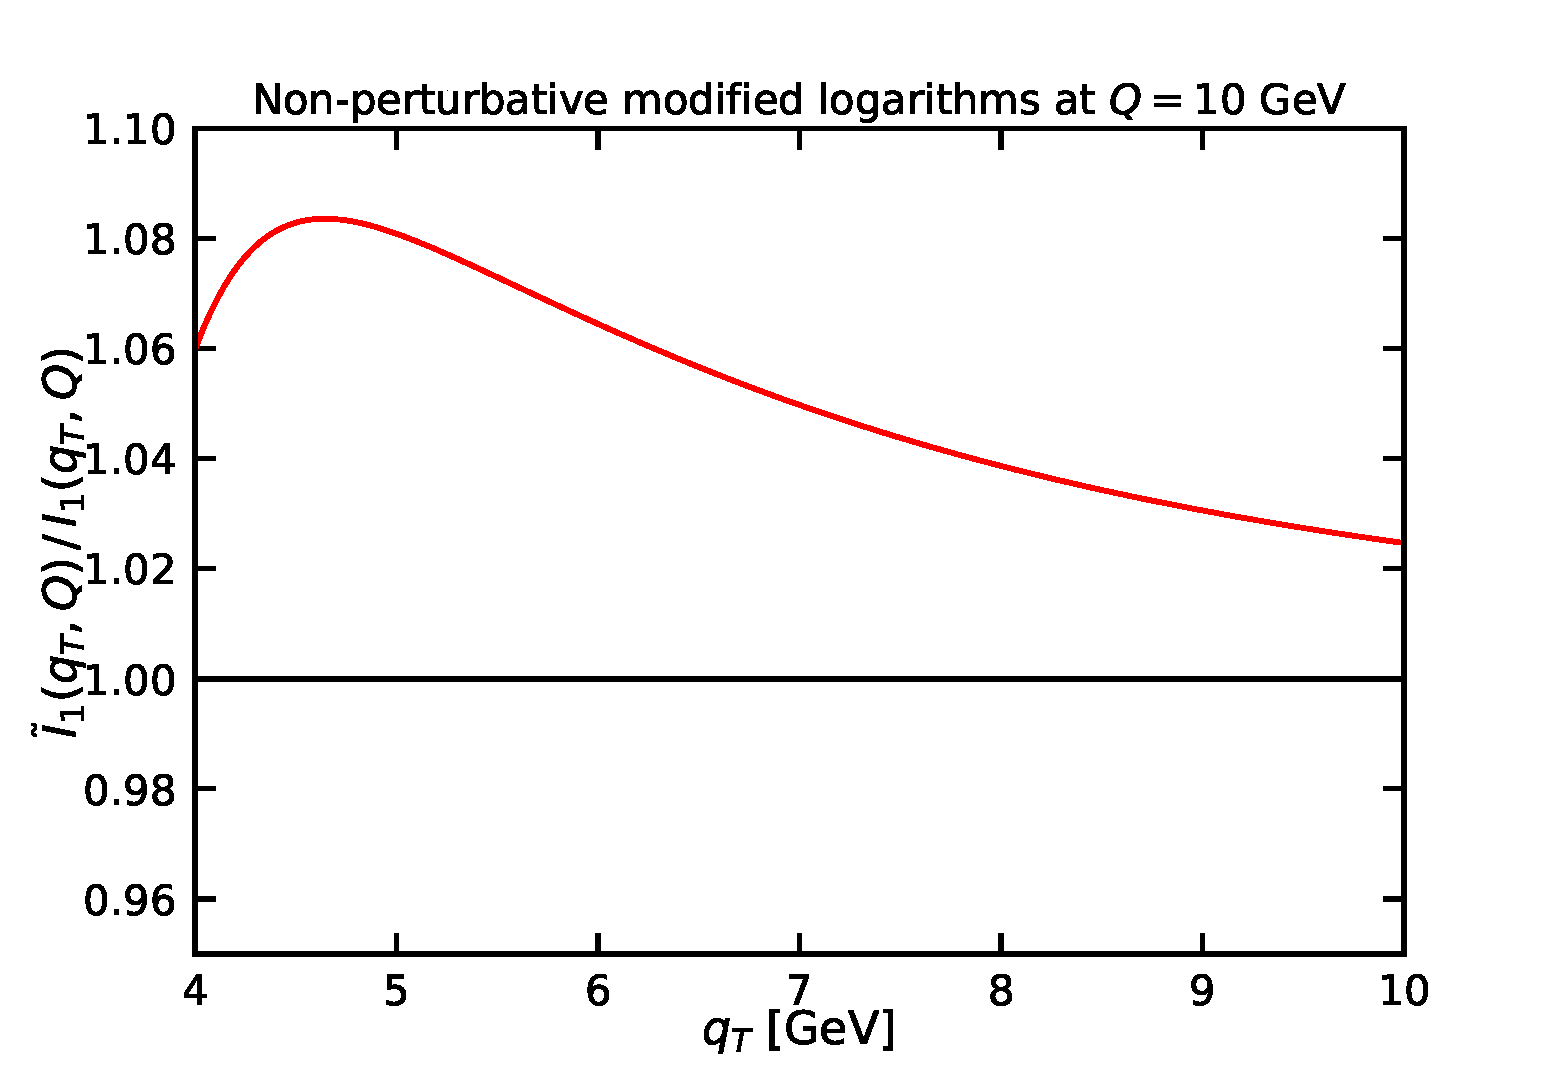
\includegraphics[width=0.45\textwidth]{plots/logsRatio.pdf}
    \caption{Ratio between $\widetilde{I}_1$ and $I_1$ in the region
      of $q_T$ close to $Q$.\label{fig:logsRatio}}
  \end{centering}
\end{figure}
In Fig~\ref{fig:logsRatio} the zoom is showed for $p=1$. Even if $q_T$
is abundantly in the fixed-order region, the difference between
$\widetilde{I}_1$ and $I_1$ is still large. Therefore, it appears that
the relation in Eq.~(\ref{eq:LogAsympt}) is not plainly
fulfilled. Moreover, the discrepancy tends to become larger as $p$
increases. Therefore, when performing the matching between resummed
and fixed-order cross sections, it is very important to include
non-perturbative effects in the expanded calculation in order to
ensure a proper cancellation with the resummed calculation in the
large-$q_T$ region.

On the other hand, by design, the inclusion of the non-perturbative
effects modifies significantly also the low-$q_T$ region. The
modification is such to prevent the cancellation at small $q_T$
between the expansion of the resummed calculation and the fixed-order
one. A possible solution is to use yet another definition of the
functions $I_p$ in the expanded calculation. These functions have to
be such to tend to those in Eq.~(\ref{eq:PureLogs}) for small values
of $q_T$ but converge to the definition in Eq.~(\ref{eq:IkNonPert})
more rapidly as $q_T$ increases. To do this, one may exploit the fact
that power-suppressed contributions do not affect the logarithmic
expansion of the resummed calculation to combine the two definitions
as follows:
\begin{equation}
\hat{I}_p(x,z,q_T,Q) =
\left[1-\left(\frac{q_T}{Q}\right)^S\right]I_p(q_T,Q) +
\left(\frac{q_T}{Q}\right)^S\widetilde{I}_p(x,z,q_T,Q)\,,
\label{eq:logsTrans}
\end{equation}
where the exponent $S$ can be adjusted to make the transition from one
regime to the other more or less strong. Clearly, this definition
should not be pushed to values of $q_T$ much above $Q$. As an example,
Fig.~\ref{fig:logsTrans} shows the shape of $\hat{I}_1$ defined in
Eq.~(\ref{eq:logsTrans}) for $S = 0.2$ along with its components given
in Eqs.~(\ref{eq:PureLogs}) and~(\ref{eq:IkNonPert}).
\begin{figure}[h]
  \begin{centering}
    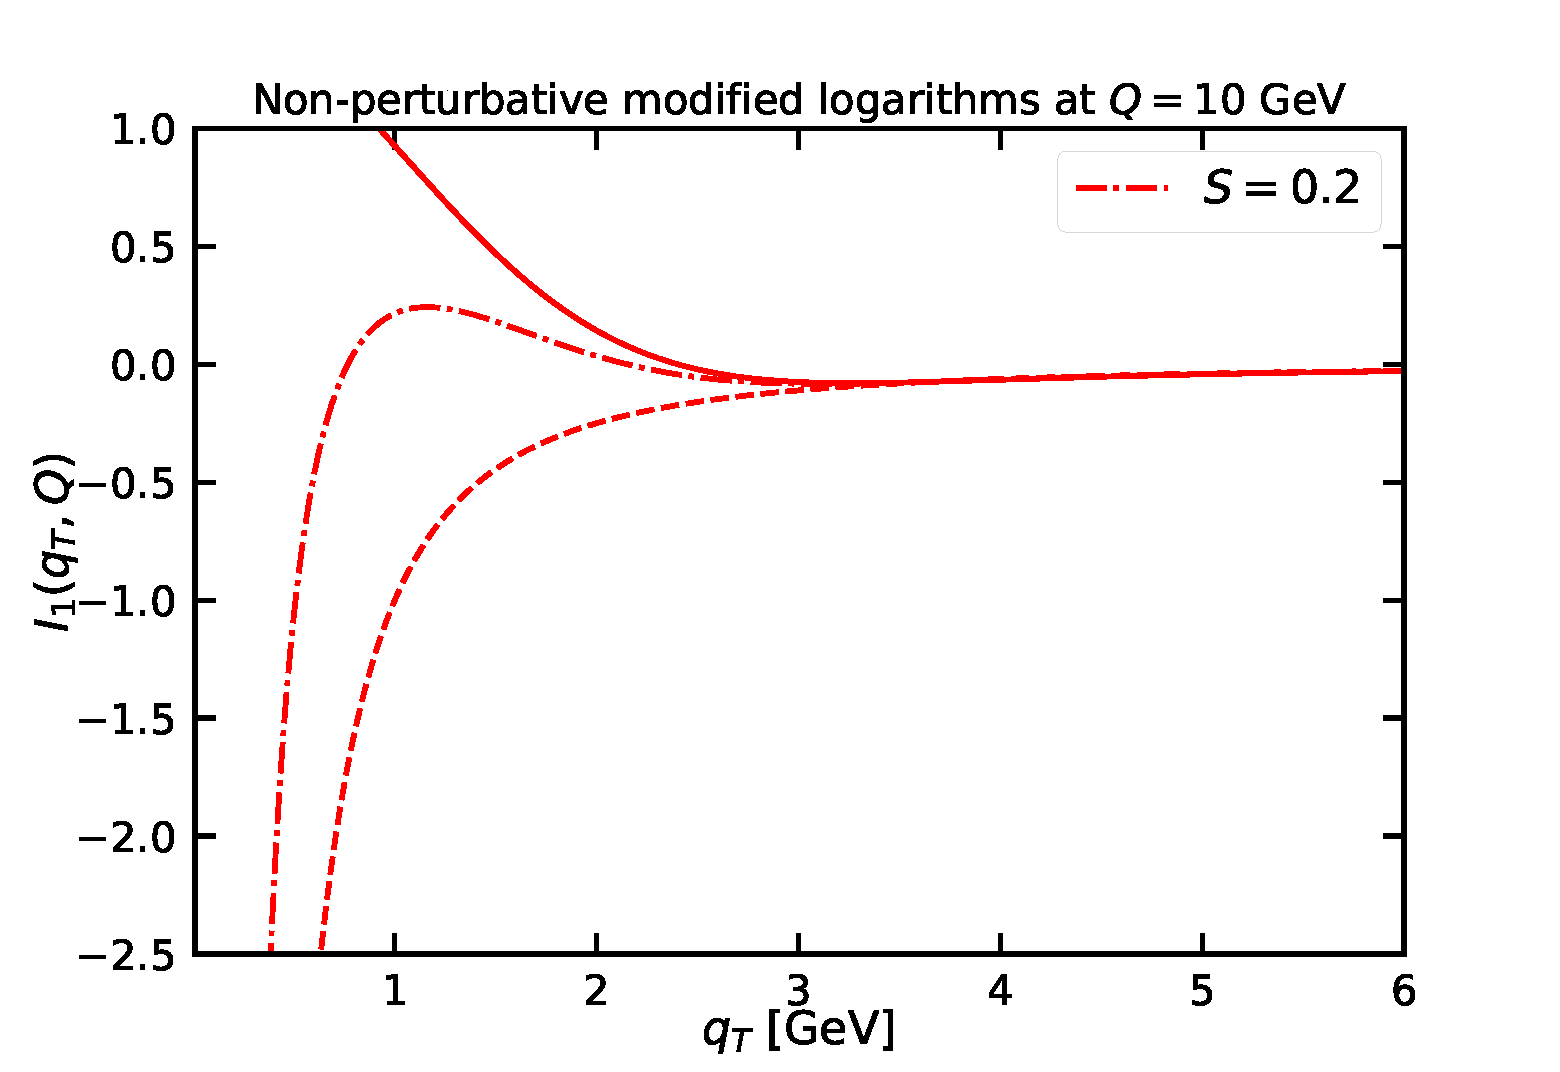
\includegraphics[width=0.45\textwidth]{plots/logsTrans.pdf}
    \caption{Behaviour of $\hat{I}_1$ defined in
      Eq.~(\ref{eq:logsTrans}) for $S = 0.2$ compared to the single
      components defined in Comparison of the integral in
      Eqs.~(\ref{eq:PureLogs})
      and~(\ref{eq:IkNonPert}).\label{fig:logsTrans}}
  \end{centering}
\end{figure}

\section{Resummation scheme}

The resummed cross section in
Eqs.~(\ref{eq:qTspectrum})-(\ref{eq:xsecexp}) is written in terms of
process-independent TMDs, $F$ and $D$, and a hard factor $H$ that is
instead process dependent. However, in the original $q_T$-resummation
formalism applied to Drell-Yan production the same cross section was
written in a different but equivalent way as:
\begin{equation}
\begin{array}{rcl}
  \displaystyle \frac{d\sigma}{dq_T^2} &\propto&\displaystyle  \sum_{ij}\int \frac{d^2\mathbf{b}_T}{4\pi} e^{i \mathbf{b}_T\cdot
                                                 \mathbf{q}_T} \widetilde{R}^2\left[(\mu_b,\mu_b^2)\rightarrow
                                                 (Q,Q^2)\right] \\
  \\
                                       &\times&\displaystyle \sum_{k}\left[ \widetilde{\mathcal{C}}_{ik}(x;\mu_b,\mu_b^2)\otimes
                                                f_k(x,\mu_b)\right]\sum_{l}\left[
                                                \widetilde{\mathbb{C}}_{jl}(z;\mu_b,\mu_b^2)\otimes
                                                d_l(z,\mu_b)\right]\,,
\end{array}
\label{eq:xsecexpqTres}
\end{equation}
where there is no hard function $H$ and the Sudakov form factor
$\widetilde{R}^2$ as well as the matching functions
$\widetilde{\mathcal{C}}$ and $\widetilde{\mathbb{C}}$ are now process
dependent. The correspondence between the various ingredients of
Eqs.~(\ref{eq:xsecexp}) and~(\ref{eq:xsecexpqTres}) requires that:
\begin{equation}
  H(Q)R^2(Q, \mu_b) \mathcal{C}(\mu_b) \mathbb{C}(\mu_b)=\widetilde{R}^2(Q,\mu_b)
  \widetilde{\mathcal{C}}(\mu_b)\widetilde{\mathbb{C}}(\mu_b)\,,
\label{eq:resschemeequiv}
\end{equation}
where we only indicated the relevant scales, and can be established by
considering the RGE of the hard factor $H$. Dropping the flavour
indices and considering that $H(\mu)=H(a_s(\mu))$ with
$a_s=\alpha_s/4\pi$, the chain rule gives the following differential
equation:
\begin{equation}
\frac{d\ln H}{d\ln\mu}=\frac{d\ln a_s}{d\ln \mu}\frac{d\ln H}{d\ln
  a_s} = -2\beta(a_s)H^{-1}\frac{dH}{d a_s}\,,
\end{equation}
whose solution is:
\begin{equation}
H(Q) = H(\mu_0)\exp\left[-2\int_{\mu_0}^{Q}\frac{d\mu}{\mu}\beta(a_s(\mu))H^{-1}(\mu)\frac{dH (\mu)}{da_s}\right]\,.
\label{eq:Hevol}
\end{equation}
Setting $\mu_0=\mu_b = 2e^{-\gamma_E}/b_T$ and replacing $H(Q)$ in the
l.h.s. of Eq.~(\ref{eq:resschemeequiv}) with the r.h.s. of
Eq.~(\ref{eq:Hevol}) allows us to write:
\begin{equation}
  H(Q)R^2(Q, \mu_b) \mathcal{C}(\mu_b) \mathbb{C}(\mu_b)= R^2(Q, \mu_b)\exp\left[-2\int_{\mu_b}^{Q}\frac{d\mu}{\mu}\beta(a_s(\mu))H^{-1}(\mu)\frac{dH (\mu)}{da_s}\right] [H(\mu_b)]^{1/2}\mathcal{C}(\mu_b) [H(\mu_b)]^{1/2}\mathbb{C}(\mu_b)\,,
\end{equation}
so that we can identify:
\begin{equation}
\begin{array}{rcl}
  \displaystyle \widetilde{R}(Q,\mu_b)&=&\displaystyle R(Q, \mu_b)\exp\left[-\int_{\mu_b}^{Q}\frac{d\mu}{\mu}\beta(a_s(\mu))H^{-1}(\mu)\frac{dH (\mu)}{da_s}\right]\,,\\
  \\
  \displaystyle \widetilde{\mathcal{C}}(\mu_b)&=&\displaystyle
                                                  [H(\mu_b)]^{1/2}\mathcal{C}(\mu_b) \,,\\
  \\
  \displaystyle \widetilde{\mathbb{C}}(\mu_b)&=&\displaystyle
                                                 [H(\mu_b)]^{1/2}\mathbb{C}(\mu_b) \,.\\
\end{array}
\label{eq:qTresToTMD}
\end{equation}
Given Eq.~(\ref{eq:evkernelexp}), the identification of the Sudakov
form factor is equivalent to the following change of the non-cusp
anomalous dimension:
\begin{equation}
\widetilde{\gamma}_F(a_s(\mu)) = \gamma_F(a_s(\mu))
-\beta(a_s(\mu))H^{-1}(\mu)\frac{dH (\mu)}{da_s}\,.
\label{eq:noncusptransf}
\end{equation}
The relations above define a particular \textit{resummation scheme}
trasformation that leaves the cross section unchanged. In fact, there
is an infinite number of possible resummation scheme
trasformations. Given any perturbative function $h(a_s(\mu))$, the
cross section in Eq.~(\ref{eq:xsecexp}) is invariant under the
following tranformations:
\begin{equation}
\begin{array}{rcl}
  \displaystyle {H}(Q)&\rightarrow&h^{-1}(Q)H(Q)\,,\\
  \\
  \displaystyle \gamma_F(a_s(\mu)) &\rightarrow& \displaystyle \gamma_F(a_s(\mu)) -\beta(a_s(\mu))h^{-1}(\mu)\frac{dh (\mu)}{da_s}\,,\\
  \\
  \displaystyle {\mathcal{C}}(\mu_b)&\rightarrow&\displaystyle
                                                  [h(\mu_b)]^{1/2}\mathcal{C}(\mu_b) \,,\\
  \\
  \displaystyle {\mathbb{C}}(\mu_b)&\rightarrow&\displaystyle
                                                 [h(\mu_b)]^{1/2}\mathbb{C}(\mu_b) \,.\\
\end{array}
\end{equation}
The particular choice $h=H$ gives the transformations in
Eqs.~(\ref{eq:qTresToTMD}) and~(\ref{eq:noncusptransf}). These
tranformations can be expanded up to the nominal order such that to
N$^3$LL the relevant shifts of the perturbative coefficients are:
\begin{equation}
\begin{array}{rcl}
\displaystyle \widetilde{\mathcal{C}}_{ij}^{(0)}(x) &=&\displaystyle
                                                \mathcal{C}_{ij}^{(0)}(x)=\delta_{ij}\delta(1-x)\,,\\
\\
\displaystyle \widetilde{\mathcal{C}}_{ij}^{(1)}(x) &=&\displaystyle
                                                \mathcal{C}_{ij}^{(1)}(x)+\frac12 H^{(1)}\delta_{ij}\delta(1-x) \,,\\
\\
\displaystyle \widetilde{\mathcal{C}}^{(2)}(x) &=&\displaystyle
                                                \mathcal{C}_{ij}^{(2)}(x)+\frac12 H^{(1)} \mathcal{C}_{ij}^{(1)}(x) +\frac12\left[H^{(2)}-\frac14(H^{(1)})^2\right]\delta_{ij}\delta(1-x) \,,
\end{array}
\end{equation}
and similarly for $\widetilde{\mathbb{C}}$, while:
\begin{equation}
\begin{array}{rcl}
\displaystyle \widetilde{\gamma}_F^{(0)} &=&\displaystyle \gamma_F^{(0)}\,,\\
\\
\displaystyle \widetilde{\gamma}_F^{(1)} &=&\displaystyle \gamma_F^{(1)}-\beta_0H^{(1)}\,,\\
\\
\displaystyle \widetilde{\gamma}_F^{(2)} &=&\displaystyle \gamma_F^{(2)}-\beta_1H^{(1)}-2\beta_0\left[H^{(2)}-\frac12 (H^{(1)})^2\right]\,.
\end{array}
\end{equation}

\subsection{Non-equivalence of resummation schemes beyond accuracy}

In this section, we explicitly show that a change of resummation
scheme leads to differences that are beyond the nominal accuracy. To
this purpose, we restrict ourselves to considering NNLL accuracy and
prove that the expansions required to implement a change of scheme
lead to order $\mathcal{O}(\alpha_s^2)$ mismatch terms. Such
corrections are of the kind $\alpha_s^{k}L^{2k-4}$ and are clearly
beyond NNLL accuracy.\footnote{Note that it may look like that this
  correction is a N$^4$LL one. However, for exponentiating observables
  the counting is best done at the level of the cumulant cross section
  which translates this term into a N$^3$LL correction.}  The proof is
simply achieved by using the equivalent of the equality in
Eq.~(\ref{eq:Hevol}) for a generic scheme-change function $h$ that we
write as follows:
\begin{equation}
h(Q) =
\left[\sqrt{h(\mu_b)}\right]^2\exp\left[-2\int_{\mu_b}^{Q}\frac{d\mu}{\mu}\beta(a_s(\mu))h^{-1}(\mu)\frac{dh
    (\mu)}{da_s}\right]\,,
\label{eq:Hevolsplit}
\end{equation}
as a consequence of the fact that each of the two $\sqrt{h(\mu_b)}$ is
absorbed into one of the matching functions $C$. At NNLL it is
sufficient to limit to $\mathcal{O}(\alpha_s)$ corrections to $h$:
\begin{equation}
h(\mu) = 1 + a_s(\mu)h^{(1)}\,,
\end{equation}
such that:
\begin{equation}
\sqrt{h(\mu_b)} = 1 + \frac{1}{2}a_s(\mu_b)h^{(1)}+\mathcal{O}(\alpha_s^2)\,,
\end{equation}
and:
\begin{equation}
\beta(a_s(\mu))h^{-1}(\mu)\frac{dh (\mu)}{da_s} = a_s^2(\mu)h^{(1)}\beta_0+\mathcal{O}(\alpha_s^3)\,.
\end{equation}
We also need to expand the running of $\alpha_s$:
\begin{equation}
a_s(\mu) = a_s(\mu_0)-2a_s^2(\mu_0)\beta_0\ln\frac{\mu}{\mu_0}+\mathcal{O}(\alpha_s^3)\,,
\label{eq:alphasexpagain}
\end{equation}
that allows us to write:
\begin{equation}
\exp\left[-2\int_{\mu_b}^{Q}\frac{d\mu}{\mu}\beta(a_s(\mu))h^{-1}(\mu)\frac{dh (\mu)}{da_s}\right] = 1-2a_s^2(\mu_b)h^{(1)}\beta_0\ln\frac{Q}{\mu_b}+\mathcal{O}(\alpha_s^3)\,.
\end{equation}
so that the r.h.s. of Eq.~(\ref{eq:Hevolsplit}) can be expanded as:
\begin{equation}
\left[\sqrt{h(\mu_b)}\right]^2\exp\left[-2\int_{\mu_b}^{Q}\frac{d\mu}{\mu}\beta(a_s(\mu))h^{-1}(\mu)\frac{dh
    (\mu)}{da_s}\right] = 1 +
a_s(\mu_b)h^{(1)}+a_s^2(\mu_b)h^{(1)}\left(\frac{1}{4}h^{(1)}-2\beta_0\ln\frac{Q}{\mu_b}\right)+\mathcal{O}(\alpha_s^3)\,.
\label{eq:Hevolrhs}
\end{equation}
Now we use Eq.~(\ref{eq:alphasexpagain}) to expand the l.h.s. of
Eq.~(\ref{eq:Hevolsplit}) as follows:
\begin{equation}
h(Q) = 1 + a_s(\mu_b)h^{(1)}-2a_s^2(\mu_0) h^{(1)}\beta_0\ln\frac{\mu}{\mu_0}+\mathcal{O}(\alpha_s^3)\,.
\label{eq:Hevollhs}
\end{equation}
Finally, taking the difference between l.h.s. and r.h.s. of
Eq.~(\ref{eq:Hevolsplit}) one immediately finds:
\begin{equation}
h(Q) -
\left[\sqrt{h(\mu_b)}\right]^2\exp\left[-2\int_{\mu_b}^{Q}\frac{d\mu}{\mu}\beta(a_s(\mu))h^{-1}(\mu)\frac{dh
    (\mu)}{da_s}\right] = -\left[\frac12a_s(\mu_b)h^{(1)}\right]^2+\mathcal{O}(\alpha_s^3)=\mathcal{O}(\alpha_s^2)\,.
\end{equation}
This confirms that a resummation-scheme change at NNLL leads to
non-vanishing differences that are however beyond accuracy. This is a
particular case of a result that is extensible to all fixed
logarithmic orders.












\newpage

\part{Semi-inclusive deep-inelastic-scattering}

\section{Fixed order and asymptotic limit}

In order to validate the results above, it is opportune to compare the
$\mathcal{O}(a_s)$ expressions to those present in the literature. To
this end, we write explicitly the expression for the SIDIS cross
section differential in $q_T$ for $q_T>0$, \textit{i.e.} without the
$\delta(q_T^2)$ terms, and with no non-perturbative
effect. Considering that, $S^{(1,1)} = 6C_F$, $S^{(1,2)} = -2C_F$, and
$H_{ij}^{(0)} = e_i^2\delta_{ij}$, this yields:
\begin{equation}
\begin{array}{rcl}
  \displaystyle  \frac{d\sigma}{dx dy dz dq_T^2} &\propto &\displaystyle a_s(Q)\sum_{ij,kl}\left[
                                                   -{B}_{ij,kl}^{(1,1)}(x,z)\frac{1}{q_T^2}
                                                   -{B}_{ij,kl}^{(1,2)}(x,z)\frac{2}{q_T^2}\ln\left(\frac{Q^2}{q_T^2}\right)\right]\mathop{\otimes}_x f_k(x,Q) \mathop{\otimes}_z d_l(z,Q)\\
  \\
                                        &=&\displaystyle
                                            \frac{a_s(Q)}{q_T^2}\sum_{ij,kl}e_i^2\delta_{ij}\bigg[4C_F\left(\ln\left(\frac{Q^2}{q_T^2}\right)-\frac{3}{2}\right)\delta_{ik}\delta_{jl}\delta(1-x)\delta(1-z)\\
  \\
                                        &+&\displaystyle
                                            \mathcal{P}_{ik}^{(0)}(x)\delta_{jl}\delta(1-z)
                                            +
                                            \delta_{ik}\delta(1-x)\mathbb{P}_{jl}^{(0)}(z)\bigg]\mathop{\otimes}_x
                                            f_k(x,Q) \mathop{\otimes}_z
                                            d_l(z,Q)\\
  \\
                                        &=&\displaystyle \frac{a_s(Q)}{q_T^2}\sum_{i}e_i^2\bigg[4C_F\left(\ln\left(\frac{Q^2}{q_T^2}\right)-\frac{3}{2}\right) f_i(x,Q)d_i(z,Q)\\
  \\
                                        &+&\displaystyle \left(\sum_{k}\mathcal{P}_{ik}^{(0)}(x) \mathop{\otimes}_x
                                            f_k(x,Q)\right)d_i(z,Q) + f_i(x,Q)\left(\sum_l\mathbb{P}_{il}^{(0)}(z) \mathop{\otimes}_zd_l(z,Q)\right)\bigg] +\mathcal{O}(a_s^2)\,.
\end{array}
\label{eq:asymptfromres}
\end{equation}
This result, up to pre-factors that will be made explicit below,
nicely agrees with that of, \textit{e.g.},
Refs.~\cite{Meng:1995yn,Collins:2016hqq,Nadolsky:1999kb}.

In order to check that the matching is actually removing the double
counting terms, it is instructive to derive
Eq.~(\ref{eq:asymptfromres}) extracting the asymptote from the
fixed-order computation at $\mathcal{O}(a_s)$. We take the expressions
for the coefficient functions from Eqs.~(106)-(109) of Appendix B of
Ref.~\cite{Nadolsky:1999kb} or from Eqs.~(4.6)-(4.20) of
Ref.~\cite{Bacchetta:2008xw}. Referring to the second reference, some
simplifications apply. In particular, we consider cross sections with
unpolarised projectiles ($\lambda_e=0$) on unpolarised targets
($S_\perp^\mu = 0$) and integrated over the azimuthal angles $\phi_H$
and $\phi_S$. By doing so and after a simple manipulation, the cross
section simplifies greatly and can be written in terms of structure
functions as:
\begin{equation}
  \frac{d\sigma}{dx dy dz dq_T^2} =
  \frac{2\pi\alpha^2}{xyQ^2}\left[Y_+
    F_{UU,T}+2(1-y)F_{UU,L}\right]=\frac{2\pi\alpha^2}{xyQ^2}Y_+\left[F_{UU,2}-\frac{y^2}{Y_+}F_{UU,L}\right]\,,
\label{eq:xsexinsf}
\end{equation}
with:
\begin{equation}
Y_+\equiv 1+(1-y)^2\,,
\end{equation}
and where we have defined the structure function:
\begin{equation}
F_{UU,2}\equiv F_{UU,T} + F_{UU,L}\,.
\end{equation}
Notice that, as compared to Ref.~\cite{Bacchetta:2008xw}, we have
factored out from the structure functions a factor
$1/(\pi z^2)$(\footnote{The factor $z^{2}$ is the consequence of the
  fact that we are writing the cross section differential in $q_T^2$
  that is the transverse momentum of the exchanged photon while in
  Ref.~\cite{Bacchetta:2008xw} the cross section is differentila in
  $p_T^2$ that is the transverse momentum of the of the outgoing
  hadrons. Since $p_T=z q_T$, the factor $z^2$ cancels.}) so that they
factorize as:
\begin{equation}
\begin{array}{rcl}
  F_{UU,S}&=&\displaystyle 
  a_s\frac{x}{Q^2}\sum_{i}e_i^2\int_x^1\frac{d\bar{x}}{\bar{x}}\int_z^1\frac{d\bar{z}}{\bar{z}}\delta\left(\frac{q_T^2}{Q^2}-\frac{(1-\bar{x})(1-\bar{z})}{\bar{x}\bar{z}}\right)\bigg[\hat{B}_{qq}^{S,
    \rm FO}(\bar{x},\bar{z},q_T)f_i\left(\frac{x}{\bar{x}}\right)
              d_i\left(\frac{z}{\bar{z}}\right)\\
\\
&+&\displaystyle \hat{B}_{qg}^{S,
    \rm FO}(\bar{x},\bar{z},q_T)f_g\left(\frac{x}{\bar{x}}\right)
              d_i\left(\frac{z}{\bar{z}}\right)+ \hat{B}_{gq}^{S,
    \rm FO}(\bar{x},\bar{z},q_T)f_i\left(\frac{x}{\bar{x}}\right)
              d_g\left(\frac{z}{\bar{z}}\right)\bigg]
+\mathcal{O}(a_s^2)\,.
\end{array}
\label{eq:FOxsec}
\end{equation}
with $S=2,L$ and where the sum over $i$ runs over the active quark and
antiquark flavours. The explicit expressions for the coefficient
functions are:
\begin{equation}
\begin{array}{l}
\displaystyle \hat{B}_{qq}^{2,\rm FO}(x,z,q_T) = 2C_F\left[(1-x)(1-z)+4xz+\frac{1+x^2z^2}{xz}\frac{Q^2}{q_T^2}\right]\,,\\
\\
\displaystyle \hat{B}_{qq}^{L,\rm FO}(x,z,q_T) = 8C_Fxz\,,\\
\\
\displaystyle \hat{B}_{qg}^{2,\rm FO}(x,z,q_T) = 2T_R\left[[x^2+(1-x)^2][z^2+(1-z)^2]\frac{1-x}{xz^2}\frac{Q^2}{q_T^2} +8x(1-x)\right]\,,\\
\\
\displaystyle \hat{B}_{qg}^{L,\rm FO}(x,z,q_T) = 16T_Rx(1-x)\,.\\
\\
\displaystyle \hat{B}_{gq}^{2,\rm FO}(x,z,q_T) = 2C_F\left[(1-x)z+4x(1-z)+\frac{1+x^2(1-z)^2}{xz}\frac{1-z}{z}\frac{Q^2}{q_T^2}\right]\,,\\
\\
\displaystyle \hat{B}_{gq}^{L,\rm FO}(x,z,q_T) = 8C_Fx(1-z)\,,
\end{array}
\label{eq:Bacchettaetal}
\end{equation}
These expressions are enough to compute the SIDIS cross section at
$\mathcal{O}(a_s)$ in the region $q_T \lesssim Q$. In order to match
Eq.~(\ref{eq:asymptfromres}), one has to take the limit
$q_T/Q\rightarrow 0$ and retain in the coefficient functions only the
terms enhanced as $\ln(Q^2/q_T^2)$. This automatically means that
$F_{UU,L}$ does not contribute in this limit because it contains no
logarithmic enhancements such that:
\begin{equation}
F_{UU,L}\mathop{\ll}_{q_T/Q\rightarrow 0} F_{UU,2}\,.
\end{equation}
Another crucial observation is that the $\delta$-function in
Eq.~(\ref{eq:FOxsec}) can be expanded as follows(\footnote{The proof of
  this relation is given in Appendix~\ref{sec:deltaexpansion}.}):
\begin{equation}
  \delta\left(\frac{q_T^2}{Q^2}-\frac{(1-x)(1-z)}{xz}\right)
  \mathop{\longrightarrow}_{q_T^2/Q^2\rightarrow0}\ln\left(\frac{Q^2}{q_T^2}\right)\delta(1-x) \delta(1-z) +
  \frac{x\delta(1-z)}{(1-x)_+}+ \frac{z\delta(1-x)}{(1-z)_+}\,,
\label{eq:deltaexpansion}
\end{equation}
so that:
\begin{equation}
\begin{array}{rcl}
  F_{UU,2}&\displaystyle \mathop{\longrightarrow}_{q_T/Q\rightarrow 0}&\displaystyle 
  a_s\frac{x}{q_T^2}\sum_{i}e_i^2\int_x^1\frac{d\bar{x}}{\bar{x}}\int_z^1\frac{d\bar{z}}{\bar{z}}\bigg[\hat{B}_{qq}^{2,
    \rm asy}(\bar{x},\bar{z},q_T)f_i\left(\frac{x}{\bar{x}}\right)
              d_i\left(\frac{z}{\bar{z}}\right)\\
\\
&+&\displaystyle \hat{B}_{qg}^{2,
    \rm asy}(\bar{x},\bar{z},q_T)f_g\left(\frac{x}{\bar{x}}\right)
              d_i\left(\frac{z}{\bar{z}}\right)+ \hat{B}_{gq}^{2,
    \rm asy}(\bar{x},\bar{z},q_T)f_i\left(\frac{x}{\bar{x}}\right)
              d_g\left(\frac{z}{\bar{z}}\right)\bigg]
+\mathcal{O}(a_s^2)\,.
\end{array}
\label{eq:FOxsecasy}
\end{equation}
with:
\begin{equation}
\begin{array}{rcl}
  \hat{B}_{qq}^{2,\rm asy}(x,z,q_T) &=& \displaystyle  2C_F\left[2
                                        \ln\left(\frac{Q^2}{q_T^2}\right)+\frac{1+x^2}{(1-x)_+}\delta(1-z) +\delta(1-x)\frac{1+z^2}{(1-z)_+} \right]\\
  \\
                                    &=&\displaystyle 2C_F\left[2\ln\left(\frac{Q^2}{q_T^2}\right) -3\right]\delta(1-x) \delta(1-z)+\mathcal{P}_{qq}^{(0)}(x)\delta(1-z)
                                        +\delta(1-x) \mathbb{P}_{qq}^{(0)}(z)\,,\\
  \\
  \hat{B}_{qg}^{2,\rm asy}(x,z,q_T) &=& \displaystyle
                                        2T_R\left[x^2+(1-x)^2\right]\delta(1-z)=\mathcal{P}_{qg}^{(0)}(x)
                                        \delta(1-z)\,,\\
\\
  \hat{B}_{gq}^{2,\rm asy}(x,z,q_T) &=& \displaystyle  \delta(1-x)2C_F\left[\frac{1+(1-z)^2}{z}\right]=\delta(1-x)\mathbb{P}_{qg}^{(0)}(z)\,.
\end{array}
\end{equation}
It is thus easy to see that we can rewrite Eq.~(\ref{eq:FOxsecasy})
as:
\begin{equation}
\begin{array}{rcl}
  F_{UU,2}&\displaystyle \mathop{\longrightarrow}_{q_T/Q\rightarrow 0}&\displaystyle 
  a_s\frac{x}{q_T^2}\sum_{i}e_i^2 \Bigg[4C_F\left(\ln\left(\frac{Q^2}{q_T^2}\right) -\frac{3}{2}\right) f_i\left(x\right)
              d_i\left(z\right)\\
\\
&+&\displaystyle
    \left(\sum_{k=q,g}\mathcal{P}^{(0)}_{ik}(x)\otimes f_k\left(x\right) \right)
              d_i\left(z\right)+ f_i\left(x\right)
              \left(\sum_{k=q,g}\mathbb{P}^{(0)}_{ik}(z) \otimes d_k\left(z\right)\right)\Bigg]
+\mathcal{O}(a_s^2)\,.
\end{array}
\label{eq:FOxsecasy2}
\end{equation}
Therefore, up to factors, Eq.~(\ref{eq:FOxsecasy2}) agrees with
Eq.~(\ref{eq:asymptfromres}). This confirms that the expansion of the
resummed calculation, as well as the asymptotic limit of the fixed
order, removes the double-counting terms when doing the matching.

In order to provide a version of Eq.~(\ref{eq:FOxsec}) that can be
readily implemented, we need to perform one of the integrals making
use of the $\delta$-function. We integrate over $\bar{x}$ so that we
write:
\begin{equation}
\delta\left(\frac{q_T^2}{Q^2}-\frac{(1-\bar{x})(1-\bar{z})}{\bar{x}\bar{z}}\right)
= \frac{\bar{z}\bar{x}_0^2}{1-\bar{z}}\delta(\bar{x} - \bar{x}_0)\,,
\end{equation}
with:
\begin{equation}
  \bar{x}_0 =
  \frac{1-\bar{z}}{1-\bar{z}\left(1-\frac{q_T^2}{Q^2}\right)}\,.
\label{eq:x0bar}
\end{equation}
This allows us to write:
\begin{equation}
\begin{array}{rcl}
  F_{UU,S}&=&\displaystyle 
  a_s\frac{x }{Q^2}\sum_{i}e_i^2\int_z^{z_{\rm max}} \frac{d\bar{z}}{1-\bar{z}}\bar{x}_0\bigg[\hat{B}_{qq}^{S,
    \rm FO}(\bar{x}_0,\bar{z},q_T)f_i\left(\frac{x}{\bar{x}_0}\right)
              d_i\left(\frac{z}{\bar{z}}\right)\\
\\
&+&\displaystyle \hat{B}_{qg}^{S,
    \rm FO}(\bar{x}_0,\bar{z},q_T)f_g\left(\frac{x}{\bar{x}_0}\right)
              d_i\left(\frac{z}{\bar{z}}\right)+ \hat{B}_{gq}^{S,
    \rm FO}(\bar{x}_0,\bar{z},q_T)f_i\left(\frac{x}{\bar{x}_0}\right)
              d_g\left(\frac{z}{\bar{z}}\right)\bigg]
+\mathcal{O}(a_s^2)\,,
\end{array}
\label{eq:FOxsecFin}
\end{equation}
with:
\begin{equation}
z_{\rm max} = \frac{1-x}{1-x\left(1-\frac{q_T^2}{Q^2}\right)}\,.
\end{equation}

Now we can rewrite the cross section above in such a way that it
matches that at $\mathcal{O}(a_s)$ of Ref.~\cite{Daleo:2004pn}. That
would allow us to confidently use the $\mathcal{O}(a_s^2)$ calculation
presented in that reference for the matching to the resummed
calculation. This is made tricky by the different notation used in
Ref.~\cite{Daleo:2004pn} and from the fact that in that paper the
cross section is differential in a different set of
variables. Specifically, we would like it to be differential in $x$,
$y$, $z$, and $q_T^2$ while in Ref.~\cite{Daleo:2004pn} it is
differential in $x$, $Q^2$, $\eta$, and $p_T^2$, where the last two
are the rapidity and the transverse momentum of the outgoing hadron,
respectively. Eq.~(13) of Ref.~\cite{Daleo:2004pn}, can be translated
into our notation by noticing that:
\begin{equation}
\frac{d\sigma}{dxdQ^2d p_T^2 d\eta} = \frac{x}{z Q^2}\sum_{i,j}\int_z^{z_{\rm
    max}} \frac{d\bar{z}}{1-\bar{z}}
f_i\left(\frac{x}{\bar{x}_0}\right)d_j\left(\frac{z}{\bar{z}}\right)
\frac{d\sigma_{ij}^{(1)}}{dxdQ^2d p_T^2 d\eta}+\mathcal{O}(a_s^2)\,,
\label{eq:Daleoetal}
\end{equation}
where we have exploited the $\delta$-functions in Eqs.~(18)-(20) to
get rid of the integral over $z$.(\footnote{Notice that the $z$
  variable of Ref.~\cite{Daleo:2004pn} does not coincide with our
  definition.})

The $\mathcal{O}(a_s)$ partonic cross sections in Eqs.~(18)-(20) of
Ref.~\cite{Daleo:2004pn}, setting $\varepsilon=0$, can be written as:
\begin{equation}
\frac{d\sigma_{ij}^{(1)}}{dxdQ^2d p_T^2 d\eta}=\frac{2\pi \alpha^2 a_s
  e_q^2\bar{x}_0}{x Q^4}Y_+ \left[ \underbrace{\left( F_{UU,M}^{ij}(\bar{x}_0,\bar{z})+\frac{3}{2}F_{UU,L}^{ij}(\bar{x}_0,\bar{z})\right)}_{F_{UU,2}^{ij}} - \frac{y^2}{Y_+}F_{UU,L}^{ij}(\bar{x}_0,\bar{z})\right]\,.
\end{equation}
One can verify that $F_{UU,2}^{qq}(\bar{x}_0,\bar{z})$,
$F_{UU,L}^{qq}(\bar{x}_0,\bar{z})$,
$F_{UU,M}^{qg}(\bar{x}_0,\bar{z})$,
$F_{UU,L}^{qg}(\bar{x}_0,\bar{z})$,
$F_{UU,M}^{gq}(\bar{x}_0,\bar{z})$, and
$F_{UU,L}^{gq}(\bar{x}_0,\bar{z})$ correspond exactly to
$\hat{B}^{2, \rm FO}_{qq}(\bar{x}_0,\bar{z},q_T)$,
$\hat{B}^{L, \rm FO}_{qq}(\bar{x}_0,\bar{z},q_T)$,
$\hat{B}^{M, \rm FO}_{qg}(\bar{x}_0,\bar{z},q_T)$,
$\hat{B}^{L, \rm FO}_{qg}(\bar{x}_0,\bar{z},q_T)$,
$\hat{B}^{M, \rm FO}_{gq}(\bar{x}_0,\bar{z},q_T)$, and
$\hat{B}^{L, \rm FO}_{gq}(\bar{x}_0,\bar{z},q_T)$ in
Eq.~(\ref{eq:Bacchettaetal}) of Ref.~\cite{Bacchetta:2008xw}. It is
crucial to notice that the correspondence holds only if $\bar{x}_0$
defined in Eq.~(\ref{eq:x0bar}) as a function of $\bar{z}$ is used. As
an example, taking into account the different factors (a factor 2 for
$F_{UU,M}$ and a factor 4 for $F_{UU,L}$) and using our notation for
the integration variables ($y\rightarrow \bar{z}$,
$\rho(z=0)\rightarrow \bar{x}_0$), we read off from Eq.~(18) of
Ref.~\cite{Daleo:2004pn}:
\begin{equation}
\begin{array}{rcl}
F_{UU,M}^{qq}(\bar{x}_0,\bar{z}) &=& \displaystyle 2C_F\left[\frac{(\bar{x}_0+\bar{z})^2+2(1-\bar{x}_0-\bar{z})}{(1-\bar{x}_0)(1-\bar{z})}\right]\,,\\
\\
F_{UU,L}^{qq}(\bar{x}_0,\bar{z}) &=& \displaystyle 8C_F\bar{x_0}\bar{z}\,,
\end{array}
\end{equation}
so that:
\begin{equation}
\begin{array}{rcl}
F_{UU,2}^{qq}(\bar{x}_0,\bar{z}) &=& \displaystyle F_{UU,M}^{qq}(\bar{x}_0,\bar{z})+\frac{3}{2}F_{UU,L}^{qq}(\bar{x}_0,\bar{z})\\
\\
 &=& \displaystyle 2
     C_F\left[\frac{(\bar{x}_0+\bar{z})^2+2(1-\bar{x}_0-\bar{z})}{(1-\bar{x}_0)(1-\bar{z})}
     + 3\bar{x_0}\bar{z}\right]\\
\\
&=& \displaystyle 2
     C_F\left[(1-\bar{x}_0)(1-\bar{z})+4\bar{x}_0\bar{z} +\frac{1+\bar{x}_0^2\bar{z}^2}{\bar{x}_0\bar{z}}\left(\frac{\bar{x}_0\bar{z}}{(1-\bar{x}_0)(1-\bar{z})}\right)\right]\,.
\end{array}
\end{equation}
Using Eq.~(\ref{eq:x0bar}), it is easy to see that the factor in round
brackets in the last line of the equation above is equal to
$Q^2/q_T^2$. Therefore, it reduces exactly to the first relation in
Eq.~(\ref{eq:Bacchettaetal}) of Ref.~\cite{Bacchetta:2008xw}. The same
holds also for the two remaining partonic channels.

Putting all pieces together, Eq.~(\ref{eq:Daleoetal}) can be recast as:
\begin{equation}
\frac{d\sigma}{dxdQ^2d p_T^2 d\eta} = \frac{2\pi \alpha^2
  }{z x Q^4}Y_+ \left[F_{UU,2} - \frac{y^2}{Y_+}F_{UU,L}\right]\,,
\end{equation}
with:
\begin{equation}
\begin{array}{rcl}
  F_{UU,S}&=&\displaystyle 
  a_s\frac{x }{Q^2}\sum_{i}e_i^2\int_z^{z_{\rm max}}
              \frac{d\bar{z}}{1-\bar{z}}\bar{x}_0\bigg[F^{qq}_{UU,L}(\bar{x}_0,\bar{z})f_i\left(\frac{x}{\bar{x}_0}\right)
              d_i\left(\frac{z}{\bar{z}}\right)\\
\\
&+&\displaystyle F^{qg}_{UU, L}(\bar{x}_0,\bar{z})f_g\left(\frac{x}{\bar{x}_0}\right)
              d_i\left(\frac{z}{\bar{z}}\right)+ F^{gq}_{UU, L}(\bar{x}_0,\bar{z})f_i\left(\frac{x}{\bar{x}_0}\right)
              d_g\left(\frac{z}{\bar{z}}\right)\bigg]
+\mathcal{O}(a_s^2)\,.
\end{array}
\end{equation}
Therefore, the structure of the observables is exactly the same. What
is left to work out is the Jacobian to express the cross section
differential in the same variables as in Eq.~(\ref{eq:xsexinsf}). What
we need is to know is how the variables $Q^2$, $p_T$, and $\eta$ are
related to $y$, $z$, and $q_T$. The relevant relations are:
\begin{equation}
\left\{\begin{array}{rcl}
Q^2 &=& xyS_H\\
\\
p_T^2 &=& z^2 q_T^2\\
\\
\eta &=& \displaystyle \frac{1}{2}\ln\left(\frac{y(1-x)S_H}{q_T^2}\right)
\end{array}\right.\quad\Longrightarrow\quad dQ^2dp_T^2d\eta =
\frac{zQ^2}{y} dydzdq_T^2\,.
\label{eq:variablechange}
\end{equation}
where $S_H$ is the squared center-of-mass energy of the collision, so
that:
\begin{equation}
  \frac{d\sigma}{dx dy dz dq_T^2} = \frac{zQ^2}{y}\frac{d\sigma}{dxdQ^2d p_T^2
    d\eta} =
  \frac{2\pi\alpha^2}{xyQ^2}Y_+\left[F_{UU,2}-\frac{y^2}{Y_+}F_{UU,L}\right]\,,
\label{eq:differentialversion2}
\end{equation}
exactly like in Eq.~(\ref{eq:xsexinsf}). This confirms that the
computation of Ref.~\cite{Daleo:2004pn} can be matched to the resummed
calculation provided that the correct Jacobian is taken into account.

In Fig.~\ref{fig:APFELvsTIMBA}, a comparison between the
$\mathcal{O}(\alpha_s)$ computation of Ref.~\cite{Daleo:2004pn} for
the differential cross section in Eq.~(\ref{eq:Daleoetal}),
implemented in the computer code {\tt TIMBA}, and the implementation
in the {\tt APFEL++} framework~\cite{Bertone:2017gds} of the
expressions in Eq.~(\ref{eq:FOxsecFin}) is presented. The cross
section as a function of the hadron transverse momentum $p_T$ obtained
with {\tt APFEL++} is displayed as ratios to {\tt TIMBA} for
representative values of the kinematic variables: the agreement
between the two codes is excellent. Since we will be using {\tt TIMBA}
for the NLO (\textit{i.e.} $\mathcal{O}(a_s^2)$) cross section
calculation to be matched to the NNLL resummed computation, this
provides a solid ground to start from.
\begin{figure}[t]
  \begin{centering}
    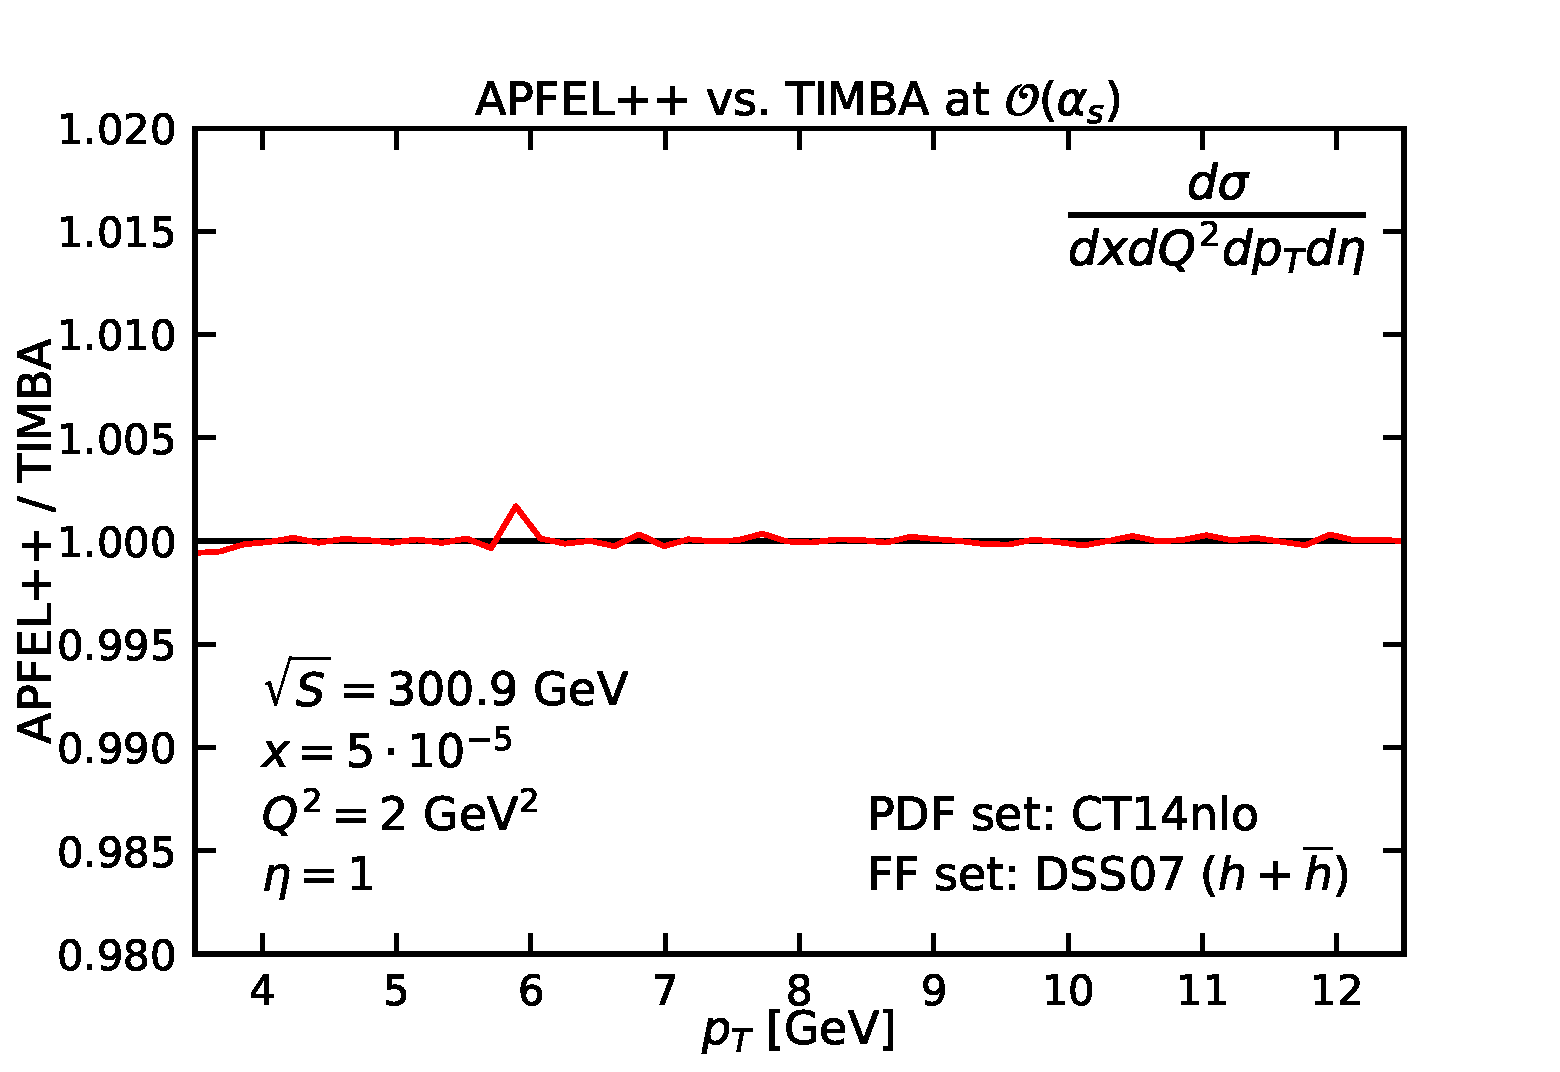
\includegraphics[width=0.5\textwidth]{plots/APFELvsTIMBA.pdf}
    \caption{Comparison at $\mathcal{O}(\alpha_s)$ between the {\tt
        TIMBA} code, implementation of the results of
      Ref.~\cite{Daleo:2004pn}, and the implementation of the
      expressions in Eq.~(\ref{eq:FOxsecFin}) in the {\tt APFEL++}
      code~\cite{Bertone:2017gds}.\label{fig:APFELvsTIMBA}}
  \end{centering}
\end{figure}

In order to be able to compare the theoretic predictions to the data,
it is useful to work out the for of the cross section differential in
the variables $x$, $Q^2$, $z$, and $p_T^2$. This is easily done
starting from Eq.~(\ref{eq:differentialversion2}) and considering
that:
\begin{equation}
\eta = \ln\left(\frac{zW}{p_T}\right)\,,\quad\mbox{with}\quad W
=\sqrt{\frac{Q^2(1-x)}{x}}\,,\quad\Rightarrow\quad d\eta = \frac{dz}{z}\,.
\end{equation}
It follows that:
\begin{equation}
 \frac{d\sigma}{dxdQ^2dz dp_T^2} =
 \frac{2\pi\alpha^2}{xQ^4}Y_+\left[F_{UU,2}-\frac{y^2}{Y_+}F_{UU,L}\right]\,,
\label{eq:differentialversion3}
\end{equation}
with $y=Q^2/xS_H$ (see Eq.~(\ref{eq:variablechange})).

% \section{Numerical results}

% The next step is to compare the asymptotic behaviour worked out in
% Eq.~(\ref{eq:FOxsecasy2}) to the fixed-order computation. This is done
% Fig.~\ref{fig:FOvsAsy} where the differential cross section in both
% cases is plotted as a function of the photon tranverve momentum $q_T$
% for a representative set of values of the kinematic variables. As
% expected, the two curves are very close to each other at small values
% of $q_T$ where the logarithmically enhanced terms dominate. At larger
% values of $q_T$ instead the two curves tend to depart indicating that
% power corrections are important in that region.
% \begin{figure}[t]
%   \begin{centering}
%     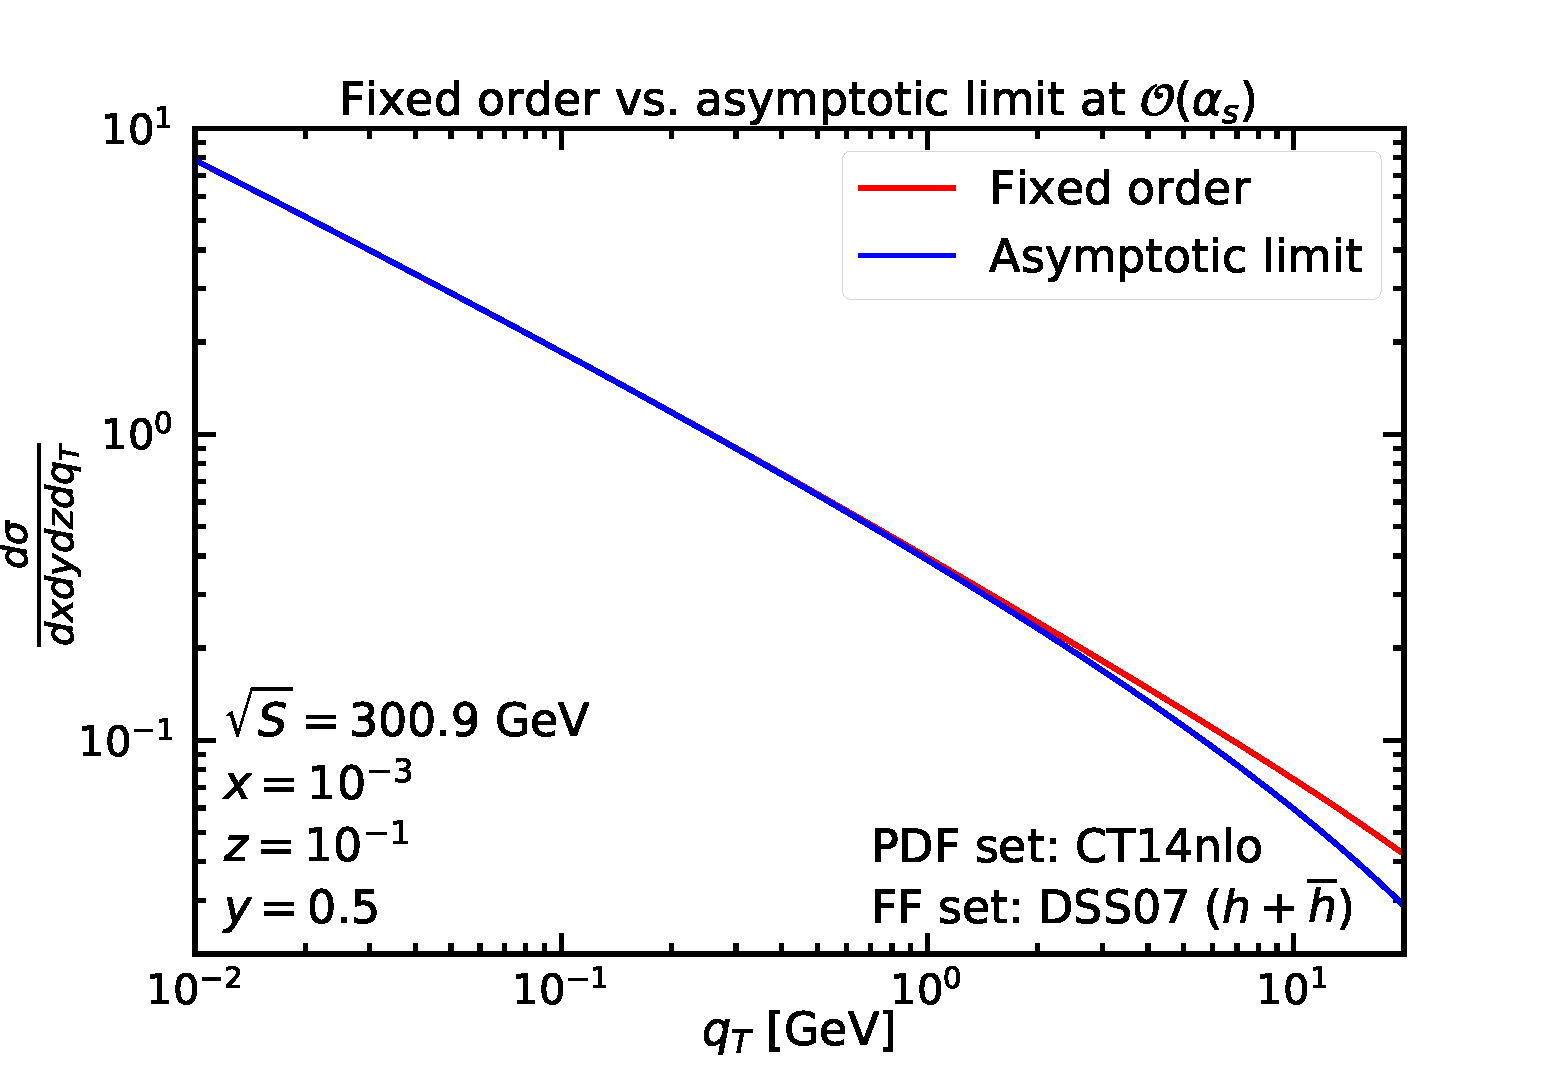
\includegraphics[width=0.6\textwidth]{plots/FOvsAsy.pdf}
%     \caption{Comparison at $\mathcal{O}(\alpha_s)$ between the
%       asymptotic limit in Eq.~(\ref{eq:FOxsecasy2}) to the fixed-order
%       computation expressions in
%       Eq.~(\ref{eq:FOxsecFin}).\label{fig:FOvsAsy}}
%   \end{centering}
% \end{figure}

% The conclusive step is the comparison between the resummed computation
% and its fixed-order order expansion that, as we have shown above,
% coincides with the asymptote of the full fixed-oder. This is done in
% Fig.~(\ref{fig:ResVsExp}) where the resummed calculation a NLL
% accuracy is compared to its fixed-order expansion to
% $\mathcal{O}(\alpha_s)$, that coincides with
% Eq.~(\ref{eq:FOxsecasy2}). As expected, while the two curves are far
% apart at low $q_T$ they tend to converge towards larger values of
% $q_T$. However, the convergence is not so ``accurate'' as in the case
% of the fixed-order calculation versus its asymptotic limit. The reason
% is that in this case the two computations converge up to subleading
% terms that in this case are $\mathcal{O}(\alpha_s^2)$ that are
% effectively NLO and thus numerically large. We will see that the
% situation improves when going one order up.
% \begin{figure}[t]
%   \begin{centering}
%     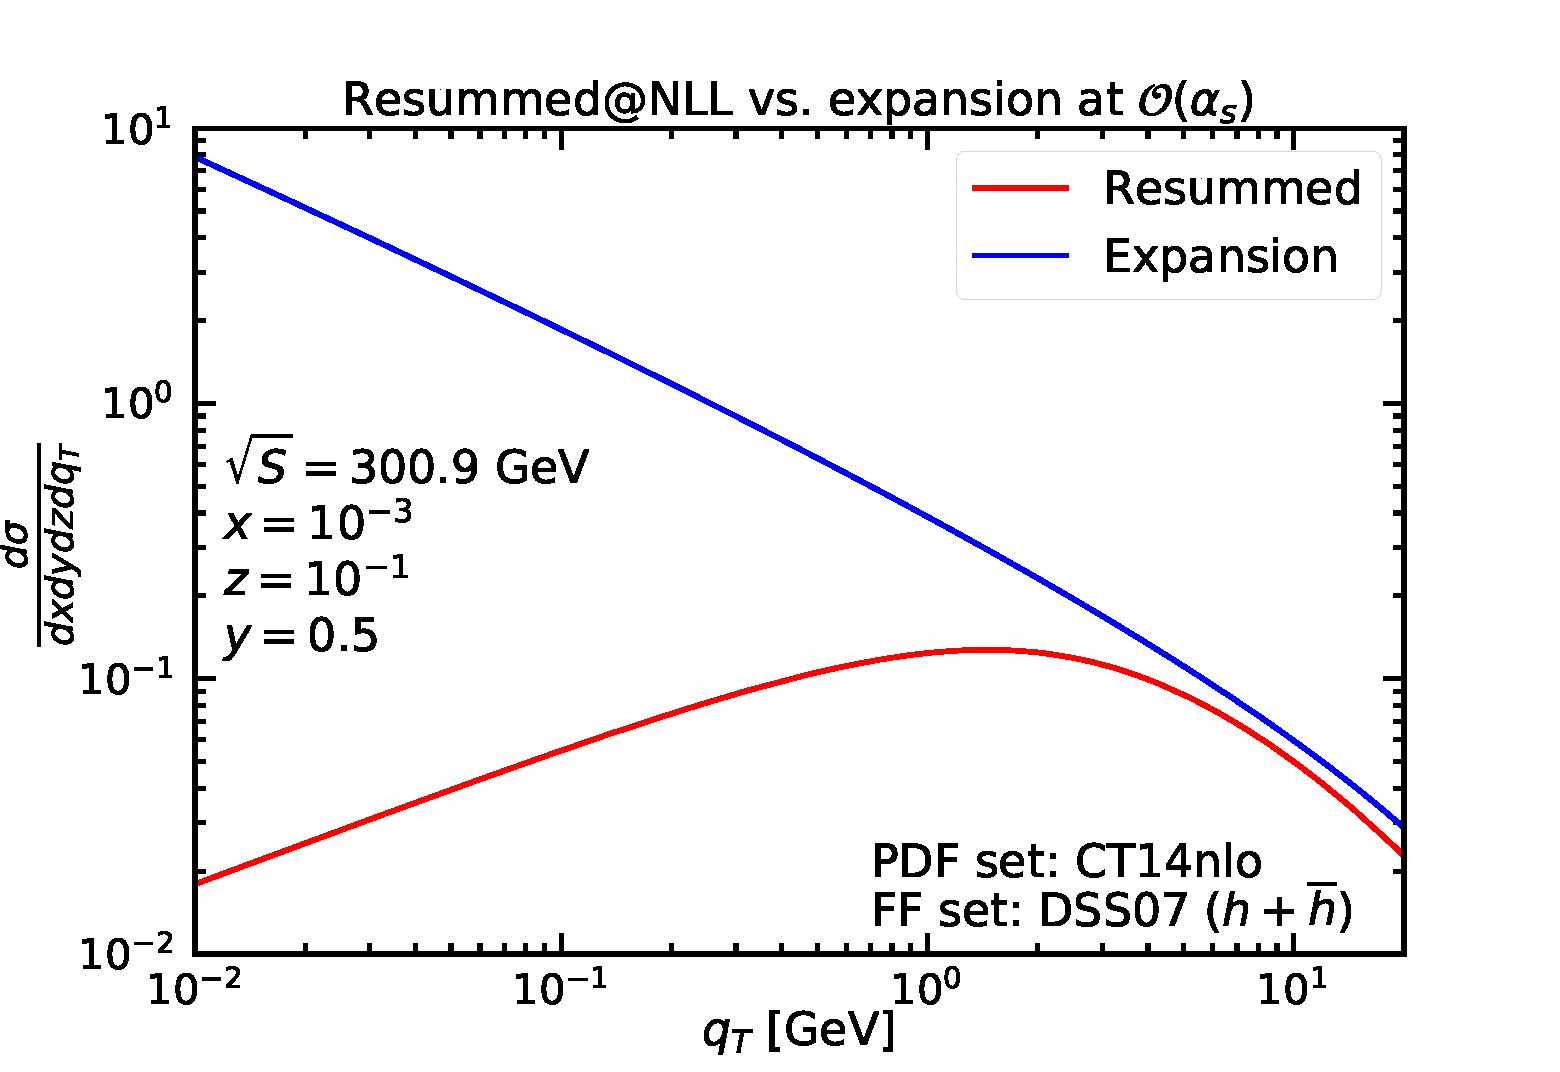
\includegraphics[width=0.6\textwidth]{plots/ResVsExp.pdf}
%     \caption{Comparison between the NLL resummed calculation and the
%       expansion to $\mathcal{O}(\alpha_s)$ in
%       Eq.~(\ref{eq:FOxsecasy2}).\label{fig:ResVsExp}}
%   \end{centering}
% \end{figure}

% We can now formulate the matching procedure to consistently combine
% the resummed calculation with the fixed-order one subtracting the
% double counting terms. The particular way in which the matching is
% implemented is defined up to subleading and power-suppressed
% terms. One can then exploit this arbitrariness to adjust the matching
% in such a way that the possibly large subleading terms are mitigated
% by some \textit{ad-hoc} prescription. The most natural, despite not
% unique, prescription is the \textit{additive} matching that reads:
% \begin{equation}\label{eq:matching1}
% \sigma^{\rm Match}(q_T,Q) = \sigma^{\rm FO}(q_T,Q) + \sigma^{\rm Res}(q_T,Q) - \sigma^{\rm Asy}(q_T,Q)\,.
% \end{equation}
% where $\sigma^{\rm Match}$ is obtained adding up the fixed-order
% computation $\sigma^{\rm FO}$ to some perturbative accuracy (say
% $\mathcal{O}(\alpha_s^n)$), valid for $q_T \simeq Q$, to the resummed
% calculation $\sigma^{\rm Res}$ at some logarithmic accuracy, valid for
% $q_T\ll Q$, and subtracting the double-counting terms
% $\sigma^{\rm Asy}$. By the arguments discussed above, it is easy to
% see that:
% \begin{equation}
% \begin{array}{rcl}
%   \sigma^{\rm Match}(q_T,Q) &\displaystyle\mathop{\longrightarrow}_{q_T\simeq Q}&
%                                                                                   \sigma^{\rm FO}(q_T,Q) +\mathcal{O}\left[\alpha_s^{n+1}(Q)\right]\,,\\
%   \\
%   \sigma^{\rm Match}(q_T,Q) &\displaystyle\mathop{\longrightarrow}_{q_T\ll Q}&\displaystyle
%                                                                                \sigma^{\rm Res}(q_T,Q) +\mathcal{O}\left(\frac{q_T^2}{Q^2}\right)\,.
% \end{array}
% \end{equation}
% However, as we have seen above, for low-order computations the
% $\mathcal{O}(\alpha_s^{n+1})$ residual for $q_T\simeq Q$ may be
% numerically relevant. On the other hand, one would expect that when
% increasing the perturbative accuracy these differences tend to
% shrink. Therefore, for the moment I refrain from form introducing any
% prescription for the suppression of subleading terms. I will come back
% on this point in the next section where I will study the matching of
% the NLO fixed-order computation to the NNLL resummed
% one. Fig.~\ref{fig:FONLL} shows a summary of the computations
% consideres so far, including the matched one according to
% Eq.~(\ref{eq:matching1}): this provides the lowest order matching
% LO+NLL. The behaviour of the red curve is the expected one. In
% particular, in the low-$q_T$ region it is close to the resummed
% (green) curve while in the high-$q_T$ region it tends to the
% fixed-order (blue) curve. In the next section we will raise the
% perturbative accuracy to NLO+NNLL.
% \begin{figure}[t]
%   \begin{centering}
%     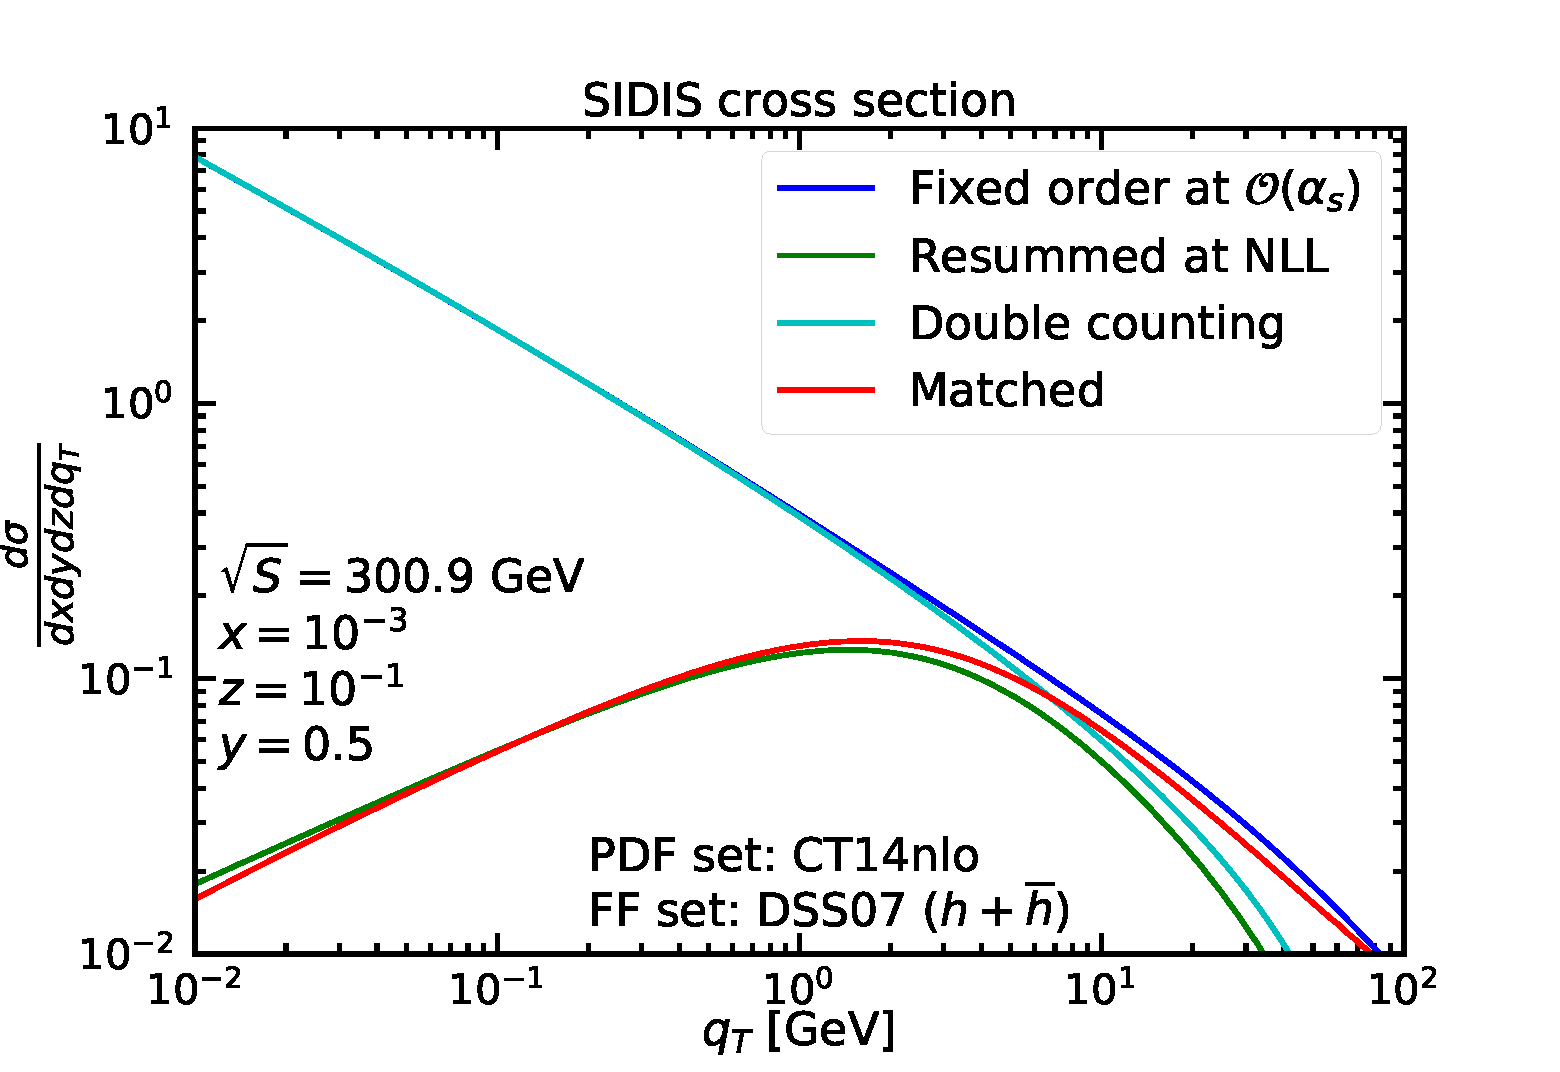
\includegraphics[width=0.6\textwidth]{plots/FONLL.pdf}
%     \caption{Summary of the computations: fixed order (blue curve),
%       resummed (green curve), double counting (cyan curve), and
%       matched according to Eq.~(\ref{eq:matching1}) (red
%       curve).\label{fig:FONLL}}
%   \end{centering}
% \end{figure}

% % Exploiting the power-suppressed residual in the $q_T \ll Q$ limit, one
% % can replace the prescription in Eq.~(\ref{eq:matching1}) with:
% % \begin{equation}\label{eq:matching2}
% %   \sigma^{\rm Match}(q_T,Q) = \sigma^{\rm FO}(q_T,Q) + \mathcal{D}\left(\frac{q_T^2}{Q^2}\right)\left[\sigma^{\rm Res}(q_T,Q) - \sigma^{\rm Asy}(q_T,Q)]\right]\,,
% % \end{equation}
% % with:
% % \begin{equation}
% % \mathcal{D}\left(\frac{q_T^2}{Q^2}\right) = 1 + \mathcal{O}\left(\frac{q_T^2}{Q^2}\right)\,.
% % \end{equation}
% % Despite the exact form of the ``damping'' function $\mathcal{D}$
% % remains unspecified at this level, this prescription ensures that the
% % uncertainty of Eq.~(\ref{eq:matching2}) is power suppressed over the
% % whole relevant spectrum. The simplest choice is:
% % \begin{equation}
% %   \mathcal{D}\left(\frac{q_T^2}{Q^2}\right) = 1 + \frac{q_T^2}{Q^2}\,.
% % \end{equation}

\section{Integrating over $q_T$}

It is interesting to carry out the integration over $q_T$ of
Eq.~(\ref{eq:FOxsec}) analytically. The result can eventually be
compared to those presented in Appendix~C of
Ref.~\cite{deFlorian:1997zj}. Exploiting the $\delta$-function yields:
\begin{equation}
\begin{array}{rcl}
  \displaystyle \int_0^{\infty} dq_T^2\,F_{UU,S}&=&\displaystyle 
                                                    a_sx\sum_{i}e_i^2\int_x^1\frac{d\bar{x}}{\bar{x}}\int_z^1\frac{d\bar{z}}{\bar{z}}\bigg[\hat{B}_{qq}^{S,
                                                    \rm FO}\left(\bar{x},\bar{z},\frac{(1-\bar{x})(1-\bar{z})}{\bar{x}\bar{z}}\right)f_i\left(\frac{x}{\bar{x}}\right)
                                                    d_i\left(\frac{z}{\bar{z}}\right)\\
  \\
                                                &+&\displaystyle \hat{B}_{qg}^{S,
                                                    \rm FO}\left(\bar{x},\bar{z},\frac{(1-\bar{x})(1-\bar{z})}{\bar{x}\bar{z}}\right)f_g\left(\frac{x}{\bar{x}}\right)
                                                    d_i\left(\frac{z}{\bar{z}}\right)\\
  \\
                                                &+& \displaystyle \hat{B}_{gq}^{S,
                                                    \rm FO}\left(\bar{x},\bar{z},\frac{(1-\bar{x})(1-\bar{z})}{\bar{x}\bar{z}}\right)f_i\left(\frac{x}{\bar{x}}\right)
                                                    d_g\left(\frac{z}{\bar{z}}\right)\bigg]
                                                    +\mathcal{O}(a_s^2)\,.
\end{array}
\end{equation}
replacing $q_T^2/Q^2$ in Eq.~(\ref{eq:Bacchettaetal}) has no effect on
the coefficient functions for $F_{UU,L}$. The reason is that
$F_{UU,L}$ is independent of $q_T$ and therefore integrating over
$q_T$ has essentially the effect of removing the $\delta$-function. On
the other hand, integrating $F_{UU,2}$ gives:
\begin{equation}
\begin{array}{l}
\displaystyle \hat{B}_{qq}^{2,\rm FO}\left(x,z,\frac{(1-{x})(1-{z})}{{x}{z}}\right) = 2C_F\left[(1-x)(1-z)+4xz+\frac{1+x^2z^2}{(1-x)(1-z)}\right]\,,\\
\\
\displaystyle \hat{B}_{qg}^{2,\rm FO}\left
  (x,z,\frac{(1-{x})(1-{z})}{{x}{z}}\right) = 2T_R\left[[x^2+(1-x)^2]\left(\frac{1}{1-z}+\frac1{z}-2\right)+8x(1-x)\right]\,,\\
\\
\displaystyle \hat{B}_{gq}^{2,\rm FO}\left (x,z,\frac{(1-{x})(1-{z})}{{x}{z}}\right) =
  2C_F\left[(1-x)z+4x(1-z)+\frac{1+x^2(1-z)^2}{z(1-x)}\right]\,,
\end{array}
\end{equation}
This expressions only account for real emissions and as a consequence
they are affected by soft divergences for $x\rightarrow 1$ and
$z\rightarrow 1$. These divergences must eventually cancel against the
virtual contributions. The inclusion of these virtual contributions
has as a net effect the appearance of the plus prescription in all
terms that behave as $(1-x)^{-1}$ and $(1-z)^{-1}$ and of terms
proportional to $\delta(1-x)$ and/or $\delta(1-z)$ (local terms). As a
matter of fact, one can see that up to the local terms and the plus
prescription the expressions of Appendix~C of
Ref.~\cite{deFlorian:1997zj} are reproduced(\footnote{The expressions
  reported in Ref.~\cite{deFlorian:1997zj} are those computed long
  time ago in Ref.~\cite{Furmanski:1981cw}.}). The local terms
correspond to virtual corrections that thus give contributions at
$q_T=0$. As such, they should coincide with the terms proportional to
$\delta(q_T^2)$ generated in the expansion of the resummed
calculation. Specifically, they should be equal to the coefficients
${B}_{ij,kl}^{(n,0)}$ in the expansion in Eq.~(\ref{eq:xsecexp}). This
is evidently the case for ${B}_{ij,kl}^{(0,0)}$ that gives the
leading-order contribution to the integrated cross
section. Unfortunately, this is not true at next-to-leading order
because the expressions for the local terms in Appendix~C of
Ref.~\cite{deFlorian:1997zj} (Eqs.~(C.2)-(C.4)) do not match
${B}_{ij,kl}^{(1,0)}$.
% However, when checking the expressions explicitly an interesting
% pattern emerges: if all the occurrences of $\ln(1-x)$ (or
% $\ln(1-z)$) in Eqs.~(C.2)-(C.4) of Ref.~\cite{deFlorian:1997zj} are
% replaced with $\ln(x)$ (or $\ln(z)$) the two sets of expressions
% coincide.
To be more precise by first writing down the explicit expression for
${B}_{ij,kl}^{(1,0)}$ summed over the indices of the hard function:
\begin{equation}
\begin{array}{rcl}
  \overline{C}_{kl}(x,z)&=&\displaystyle e_q^{-2}\sum_{ij}
                            {B}_{ij,kl}^{(1,0)}(x,z) =
                            H^{(1)}\delta_{kl}\delta(1-x)
                            \delta(1-z)+\delta(1-x)\mathbb{C}_{kl}^{(1,0)}(z)+\mathcal{C}_{lk}^{(1,0)}(x)\delta(1-z)\,,\\
\\
&=&\displaystyle 2C_F\left(-8+\frac{\pi^2}{6}\right) \delta_{kl}\delta(1-x)
                            \delta(1-z)+\delta(1-x)\mathbb{C}_{kl}^{(1,0)}(z)+\mathcal{C}_{lk}^{(1,0)}(x)\delta(1-z)\,.
\end{array}
\end{equation}
The single channels read:
\begin{equation}
\begin{array}{rcl}
  \overline{C}_{qq}(x,z) &=& \displaystyle 2C_F\left[-8\delta(1-x)
                            \delta(1-z)+\delta(1-x)\left(1-z+2 \frac{1+z^2}{1-z}\ln
                             z\right)+\left(1-x\right)\delta(1-z)\right]\,,\\
\\
  \overline{C}_{gq}(x,z) &=& \displaystyle
                             2C_F\left[\delta(1-x)\left(z+2 \frac{1+(1-z)^2}{z}\ln
                             z\right)+x\delta(1-z)\right]\,,\\
\\
  \overline{C}_{qg}(x,z)&=&\displaystyle
                            4T_R\left[\delta(1-x)\left(z(1-z)+(z^2+(1-z)^2)\ln
                            z\right)+x(1-x)\delta(1-z)\right]\,.
\end{array}
\label{eq:locals}
\end{equation}
% Confronting Eq.~(\ref{eq:locals}) with the terms proportional to the
% $\delta$-functions in Eqs.~(C.2)-(C.4) of
% Ref.~\cite{deFlorian:1997zj}, that we refer to as
% $C_{kl}^{(\rm loc)}$, we find:
% \begin{equation}
% \begin{array}{rcl}
%   C_{qq}^{(\rm loc)}(x,z)-\overline{C}_{qq}(x,z) &=& \displaystyle 2C_F\delta(1-x)(1+z^2)\left[\left(\frac{\ln(1-z)}{1-z}\right)_+-\frac{\ln(z)}{1-x}\right]\,,\\
% \\
%   C_{gq}^{(\rm loc)}(x,z)-\overline{C}_{gq}(x,z) &=& \displaystyle
%                              2C_F\left[\delta(1-x)p_{gq}(z)\ln\left(\frac{1-z} z\right)-x\delta(1-z)\right]\,,\\
% \\
%   C_{qg}^{(\rm loc)}(x,z)-\overline{C}_{qg}(x,z)&=&\displaystyle
%                             4T_R\left[-\delta(1-x)\left(z(1-z)+p_{qg}(z)\ln
%                             z\right)+p_{qg}(x)\ln\left(\frac{1-x}{x}\right)\delta(1-z)
%                             \right]\,,
% \end{array}
% \end{equation}

% In fact, the expression to $\mathcal{O}(\alpha_s)$ that we derived
% above are free of large threshold logarithms associated to soft-gluon
% emission.

\section{Integrating over $z$}

In order to understand which of the two is the correct set of
expressions, whether those computed in Ref.~\cite{Furmanski:1981cw} or
those derived here, we may try to integrate over $z$ summing over all
possible hadrons produced in the final state. By doing so, we should
obtain the expressions of the hard cross sections for inclusive
deep-inelastic scattering. This last set of expressions has also been
computed in Ref.~\cite{Furmanski:1981cw} and is very likely to be
correct. The presence of terms proportional to $\ln(1-x)$ in the
inclusive DIS hard cross sections suggests that the expressions
reported in Ref.~\cite{deFlorian:1997zj} and computed in
Ref.~\cite{Furmanski:1981cw} are the correct ones. To integrate the
expressions in Ref.~\cite{deFlorian:1997zj} we need to use the fact
that the SIDIS cross section integrate in $q_T$ for the production of
a hadron $h$ has the following structure:
\begin{equation}
\frac{d\sigma^h}{dx dy dz} = \sum_{ij} \int_x^1\frac{d\xi}{\xi}
\int_z^1\frac{d\zeta}{\zeta}
C_{ij}\left(\frac{x}{\xi},\frac{z}{\zeta}\right) d_{i/h}(\zeta)
f_j(\xi)\,,
\label{eq:intxsec}
\end{equation}
where $d_{i/h}$ is the fragmentation function for the parton $i$
fragmenting into the hadron species $h$. What we need to compute is:
\begin{equation}
\frac{d\sigma}{dx dy} = \sum_{h}\int_0^1 dz\,z\,\frac{d\sigma^h}{dx dy dz}\,,
\end{equation}
where the sum over $h$ extends over all possible hadronic species. In
order to compute the integral above we need to use the following
property of the Mellin convolution:
\begin{equation}
C(z)\otimes d(z) = \int_z^1\frac{d\zeta}{\zeta}
C\left(\frac{z}{\zeta}\right)d(\zeta) = \int_0^1d\zeta \int_0^1d\eta\,C(\zeta)f(\eta)\delta(z-\zeta\eta)\,.
\end{equation}
By using this property we have:
\begin{equation}
\begin{array}{rcl}
  \displaystyle \frac{d\sigma}{dx dy} &=& \displaystyle \sum_{ij} \int_x^1\frac{d\xi}{\xi}
                                          \int_0^1 d\zeta \,
                                          C_{ij}\left(\frac{x}{\xi},\zeta\right)f_j(\xi) \sum_h\int_0^1
                                          d\eta\,d_{i/h}(\eta)\,\int_0^1dz\,z\delta(z-\zeta\eta)\\
  \\
                                      &=& \displaystyle \sum_{j} \int_x^1\frac{d\xi}{\xi}
                                          \left[\int_0^1 d\zeta \,\zeta
                                          \sum_i  C_{ij}\left(\frac{x}{\xi},\zeta\right)\right]f_j(\xi) = \sum_{j} \int_x^1\frac{d\xi}{\xi}\,
                                          \widetilde{C}_{j}\left(\frac{x}{\xi}\right)f_j(\xi)\,.
\end{array}
\end{equation}
where we have defined the inclusive DIS coefficient functions as:
\begin{equation}
\widetilde{C}_{j}\left(\xi\right) \equiv \int_0^1 d\zeta \,\zeta
                                          \sum_i
                                          C_{ij}\left(\xi,\zeta\right)\,,
\label{eq:incDIS}
\end{equation}
and we have used the momentum sum rule:
\begin{equation}
\sum_h\int_0^1 d\eta\,\eta d_{i/h}(\eta) = 1\,,
\end{equation}
that essentially encodes the fact that the total probability for a
parton to fragment into any hadron in one. The correctness of
Eq.~(\ref{eq:incDIS}) can be verified explicitly by integrating over
$z$ the expressions reported in Appendix~C of
Ref.~\cite{deFlorian:1997zj} for both structure functions $F_2$ and
$F_L$. The leading order is trivial:
\begin{equation}
\widetilde{C}_{2,q}^{(0)}\left(\xi\right) \equiv \int_0^1 d\zeta \,\zeta
                                         \delta(1-\xi)\delta(1-\zeta) = \delta(1-\xi)\,,
\end{equation}
as well know, while the gluon as well as the longitudinal coefficient
functions are zero. The next-to-leading order coefficient functions
are computed as:
\begin{equation}
\begin{array}{l}
\displaystyle \widetilde{C}_{q}^{(1)}\left(\xi\right) \equiv \int_0^1
  d\zeta\,\zeta
  \left[C_{qq}^{(1)}\left(\xi,\zeta\right)+C_{gq}^{(1)}\left(\xi,\zeta\right)\right]\,,\\
\\
\displaystyle \widetilde{C}_{g}^{(1)}\left(\xi\right) \equiv \int_0^1
  d\zeta\,\zeta C_{qg}^{(1)}\left(\xi,\zeta\right)\,.
\end{array}
\end{equation}
For $F_L$ they read:
\begin{equation}
\begin{array}{l}
\displaystyle \widetilde{C}_{L,q}^{(1)}\left(\xi\right) = 8C_F\xi\,,\\
\\
\displaystyle \widetilde{C}_{L,g}^{(1)}\left(\xi\right) = 8T_R\xi(1-\xi)\,,
\end{array}
\end{equation}
while for $F_2$:
\begin{equation}
\begin{array}{rcl}
\displaystyle \widetilde{C}_{2,q}^{(1)}\left(\xi\right) &=&
                                                            \displaystyle 2C_F\bigg[2\left(\frac{\ln(1-\xi)}{1-\xi}\right)_+-\frac32\left(\frac{1}{1-\xi}\right)_+-(1+\xi)\ln(1-\xi)\\
\\
&-&\displaystyle \frac{1+\xi^2}{1-\xi}\ln\xi+3+2\xi-\left(\frac92+2\zeta_2\right)\delta(1-\xi)\bigg]\,,\\
\\
\displaystyle \widetilde{C}_{2,g}^{(1)}\left(\xi\right)
&=&\displaystyle 2T_R\left[(\xi^2+(1-\xi)^2)\ln\left(\frac{1-\xi}{\xi}\right)+8\xi(1-\xi)-1\right]\,.
\end{array}
\end{equation}
These expressions coincide with those reported, \textit{e.g.}, in
Chapter~4 of Ref.~\cite{Ellis:1991qj}.

\newpage

\part{Drell-Yan production}

\newpage

\appendix

\part{Appendices}

\section{Expansion of the kinematic $\delta$-function}\label{sec:deltaexpansion}

In order to prove the equality in Eq.~(\ref{eq:deltaexpansion}), we
consider the following integral:
\begin{equation}
I(\varepsilon) =\int_0^1 dx \int_0^1 dy\,\delta(xy-\varepsilon)
f(x,y)\,,
\label{eq:testint}
\end{equation}
where $f(x,y)$ is a test function ``well-behaved'' over the
integration region. Now I split the integral as follows:
\begin{equation}
I(\varepsilon) =\left(\int_0^1 dx \int_x^1 dy+\int_0^1 dy \int_y^1 dx\right)\,\delta(xy-\varepsilon) f(x,y)\,,
\end{equation}
where the first term in the r.h.s. corresponds to the integral over
the grey region \textit{above} the blue line while the second over the
grey region \textit{below} the blue line in
Fig.~\ref{fig:deltaexpansion}.
\begin{figure}[h]
  \begin{centering}
    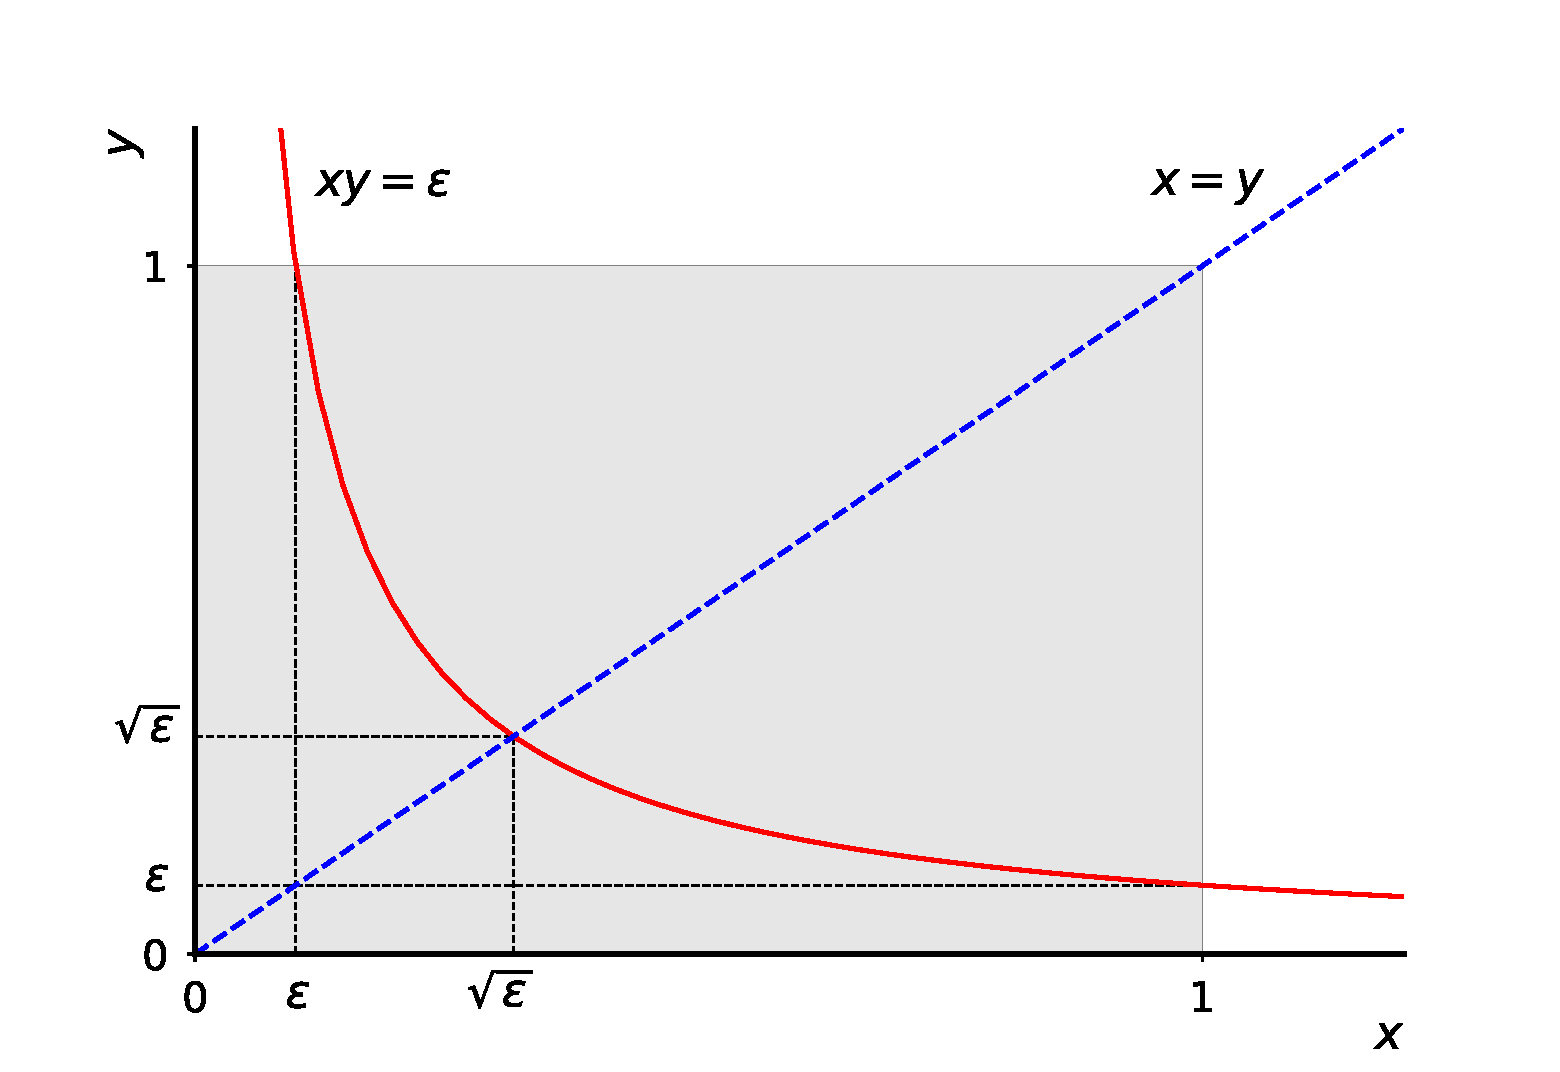
\includegraphics[width=0.5\textwidth]{plots/DeltaExpansion.pdf}
    \caption{Integration region of the integral in 
      Eq.~(\ref{eq:testint}). The integral is along the red curve 
      defined by the $\delta$-function.\label{fig:deltaexpansion}}
  \end{centering}
\end{figure}

Now I use the following equalities:
\begin{equation}
\delta(xy-\varepsilon) = \left\{
\begin{array}{ll}
\displaystyle \frac{1}{x}\delta\left(y-\frac{\varepsilon}{x}\right)\theta(y-\sqrt{\varepsilon}) &
                                                                      \quad\mbox{integral
                                                                      over
                                                                      $y$,}\\
\\
\displaystyle \frac{1}{y}\delta\left(x-\frac{\varepsilon}{y}\right) \theta(x-\sqrt{\varepsilon}) &
                                                                      \quad\mbox{integral
                                                                      over
                                                                      $x$.}
\end{array}
\right.
\end{equation}
The $\theta$-functions arise from the fact that the first integral has
to be done along the upper branch on the red curve while the second
along the lower branch. The two branches are joint at the point
$x=y=\sqrt{\varepsilon}$ and thus the integration ranges are bounded
from below by this point. Therefore, I find:
\begin{equation}
I(\varepsilon) =\int_{\sqrt{\varepsilon}}^1
\frac{dx}{x}f\left(x,\frac{\varepsilon}{x}\right) + \int_{\sqrt{\varepsilon}}^1 \frac{dy}{y}f\left(\frac{\varepsilon}{y},y\right)\,.
\end{equation}
It is crucial to realise that in the first and the second integral the
following conditions hold: $\varepsilon < \sqrt{\varepsilon}\leq x$
and $\varepsilon < \sqrt{\varepsilon}\leq y$, respectively. Therefore,
in the limit $\varepsilon\rightarrow 0$, the arguments $\varepsilon/x$
and $\varepsilon/y$ of the function $f$ will tend to zero. I now add
and subtract a term proportional to $f(0,0)$ to both integrals, so
that:
\begin{equation}
I(\varepsilon) =\int_{\sqrt{\varepsilon}}^1
\frac{dx}{x}\left[f\left(x,\frac{\varepsilon}{x}\right)-f(0,0)\right] + \int_{\sqrt{\varepsilon}}^1 \frac{dy}{y}\left[f\left(\frac{\varepsilon}{y},y\right)-f(0,0)\right]+2f(0,0) \underbrace{\int_{\sqrt{\varepsilon}}^1 \frac{d\xi}{\xi}}_{-\ln\sqrt{\varepsilon}}\,.
\end{equation}
Finally, I take the limit for $\varepsilon\rightarrow 0$:
\begin{equation}
\lim_{\varepsilon\rightarrow 0}I(\varepsilon) =\int_0^1
\frac{dx}{x}\left[f\left(x,0\right)-f(0,0)\right] + \int_{0}^1 \frac{dy}{y}\left[f\left(0,y\right)-f(0,0)\right]-\ln\left(\varepsilon\right) f(0,0)\,,
\end{equation}
that I rewrite as:
\begin{equation}
\lim_{\varepsilon\rightarrow 0}I(\varepsilon) =\int_0^1dx \int_0^1dy\left\{\frac{\delta(y)}{[x]_+}+\frac{\delta(x)}{[y]_+}-\ln\left(\varepsilon\right)\delta(x)\delta(y)\right\}f(x,y)\,.
\end{equation}
Comparing the equation above with Eq.~(\ref{eq:testint}), one deduces that:
\begin{equation}
\delta(xy-\varepsilon)\mathop{\longrightarrow}_{\varepsilon\rightarrow 0}
\frac{\delta(y)}{[x]_+}+\frac{\delta(x)}{[y]_+}-\ln\left(\varepsilon\right)\delta(x)\delta(y)\,.
\label{eq:leadinglim}
\end{equation}
Finally, substituting:
\begin{equation}
x\rightarrow \frac{1-x}{x}\,,\quad y\rightarrow
\frac{1-z}{z}\,,\quad\mbox{and}\quad\varepsilon\rightarrow\frac{q_T^2}{Q^2}\,,
\label{eq:replacements}
\end{equation}
it is easy to recover Eq.~(\ref{eq:deltaexpansion}). In particular,
one needs to use the fact that:
\begin{equation}
\delta\left(\frac{1-x}{x}\right)=\delta(1-x)\,.
\end{equation}

\subsection{Including the next corrections in $\varepsilon$}

The limit in Eq.~(\ref{eq:leadinglim}) can be written as:
\begin{equation}
  \delta(xy-\varepsilon) = 
  \frac{\delta(y)}{[x]_+}+\frac{\delta(x)}{[y]_+}-\ln\left(\varepsilon\right)\delta(x)\delta(y)
  +\mathcal{O}(\varepsilon\ln\varepsilon)\,.
\label{eq:leadingexp}
\end{equation}
The aim of this section is to calculate the first contributions to the
$\mathcal{O}(\varepsilon\ln\varepsilon)$ term: specifically we are
after terms proportional to $\varepsilon\ln\varepsilon$ and
$\varepsilon$. We start by considering the integral in
Eq.~(\ref{eq:testint}) and write:
\begin{equation}
\begin{array}{rcl}
\displaystyle J(\varepsilon) = I(\varepsilon)-\lim_{\varepsilon \rightarrow 0} I(\varepsilon) &=&\displaystyle  \int_{\sqrt{\varepsilon}}^1
\frac{dx}{x}\left[f\left(x,\frac{\varepsilon}{x}\right)-f(x,0)\right]
+ \int_{\sqrt{\varepsilon}}^1
\frac{dy}{y}\left[f\left(\frac{\varepsilon}{y},y\right)-f(0,y)\right]\\
\\

&-&\displaystyle  \int_0^{\sqrt{\varepsilon}}
\frac{dx}{x}\left[f\left(x,0\right)-f(0,0)\right] - \int_{0}^{\sqrt{\varepsilon}}
  \frac{dy}{y}\left[f\left(0,y\right)-f(0,0)\right]\,.
\end{array}
\end{equation}
We now use the following Taylor expansions(\footnote{Notice that the
  expansions in the third and fourth lines in
  Eq.~(\ref{eq:expansionsf}) are allowed because the variables $x$ and
  $y$ are bounded as $1\leq x,y \leq \sqrt{\varepsilon}$, therefore
  the ratios $\varepsilon/x$ and $\varepsilon/y$ tend to zero as
  $\varepsilon$ tends to zero over the full integration range.}):
\begin{equation}
\begin{array}{l}
\displaystyle f(x,0)=f(0,0)+\left.\frac{\partial f(x',0)}{\partial
  x'}\right|_{x'=0}x+\frac12\left.\frac{\partial^2 f(x',0)}{\partial
  x'^2}\right|_{x'=0}x^2+\mathcal{O}(x^3)\,,\\
\\
\displaystyle f(0,y)=f(0,0)+\left.\frac{\partial f(0,y')}{\partial
  y'}\right|_{y'=0}y +\frac12\left.\frac{\partial^2 f(0,y')}{\partial
  y'^2}\right|_{y'=0}y^2+\mathcal{O}(y^3)\,,\\
\\
\displaystyle f\left(x,\frac{\varepsilon}{x}\right)=f(x,0) +\left.\frac{\partial f(x,y')}{\partial
  y'}\right|_{y'=0}\frac{\varepsilon}{x}+\frac12\left.\frac{\partial^2 f(x,y')}{\partial
  y'^2}\right|_{y'=0}\frac{\varepsilon^2}{x^2}+\mathcal{O}\left(\frac{\varepsilon^3}{x^3}\right)\,,\\
\\
\displaystyle f\left(\frac{\varepsilon}{y},y\right)=f(0,y) +\left.\frac{\partial f(x',y)}{\partial
  x'}\right|_{x'=0}\frac{\varepsilon}{y}+\frac12\left.\frac{\partial^2 f(x',y)}{\partial
  x'^2}\right|_{x'=0}\frac{\varepsilon^2}{y^2}+\mathcal{O}\left(\frac{\varepsilon^3}{y^3}\right)\,,
\end{array}
\label{eq:expansionsf}
\end{equation}
so that, neglecting anything more suppressed than $\varepsilon$, we find:
\begin{equation}
\begin{array}{rcl}
\displaystyle J(\varepsilon) &=&\displaystyle  \varepsilon \int_{\sqrt{\varepsilon}}^1
\frac{dx}{x^2}\left.\frac{\partial f(x,y')}{\partial
  y'}\right|_{y'=0}
+ \frac{\varepsilon^2}{2} \int_{\sqrt{\varepsilon}}^1
\frac{dx}{x^3}\left.\frac{\partial^2 f(x,y')}{\partial
  y'^2}\right|_{y'=0}
+
\varepsilon\int_{\sqrt{\varepsilon}}^1
\frac{dy}{y^2}\left.\frac{\partial f(x',y)}{\partial
  x'}\right|_{x'=0}+\frac{\varepsilon^2}{2}\int_{\sqrt{\varepsilon}}^1
\frac{dy}{y^3}\left.\frac{\partial^2 f(x',y)}{\partial
  x'^2}\right|_{x'=0}\\
\\
&-&\displaystyle  \sqrt{\varepsilon}\left.\frac{\partial f(x',0)}{\partial
  x'}\right|_{x'=0} -\frac{\varepsilon}{4}\left.\frac{\partial^2 f(x',0)}{\partial
  x'^2}\right|_{x'=0} - \sqrt{\varepsilon}\left.\frac{\partial f(0,y')}{\partial
  y'}\right|_{y'=0}- \frac{\varepsilon}{4}\left.\frac{\partial^2 f(0,y')}{\partial
  y'^2}\right|_{y'=0}\\
\\
&=&\displaystyle \varepsilon \int_{\sqrt{\varepsilon}}^1
\frac{dx}{x^2}\left[\left.\frac{\partial f(x,y')}{\partial
  y'}\right|_{y'=0}-\left.\frac{\partial f(0,y')}{\partial
  y'}\right|_{y'=0}\right]
+ \varepsilon\int_{\sqrt{\varepsilon}}^1
\frac{dy}{y^2}\left[\left.\frac{\partial f(x',y)}{\partial
  x'}\right|_{x'=0}-\left.\frac{\partial f(x',0)}{\partial
  x'}\right|_{x'=0}\right]\\
\\
&+&\displaystyle \frac{\varepsilon^2}{2}\int_{\sqrt{\varepsilon}}^1
\frac{dx}{x^3}\left[\left.\frac{\partial^2 f(x,y')}{\partial
  y'^2}\right|_{y'=0}-\left.\frac{\partial^2 f(0,y')}{\partial
  y'^2}\right|_{y'=0}\right]
+ \frac{\varepsilon^2}{2}\int_{\sqrt{\varepsilon}}^1
\frac{dy}{y^3}\left[\left.\frac{\partial^2 f(x',y)}{\partial
  x'^2}\right|_{x'=0}-\left.\frac{\partial^2 f(x',0)}{\partial
  x'^2}\right|_{x'=0}\right]\\
\\
&+&\displaystyle \varepsilon \int_{\sqrt{\varepsilon}}^1
\frac{dx}{x^2}\left.\frac{\partial f(0,y')}{\partial
  y'}\right|_{y'=0}
+ \varepsilon\int_{\sqrt{\varepsilon}}^1
\frac{dy}{y^2}\left.\frac{\partial f(x',0)}{\partial
  x'}\right|_{x'=0}-\displaystyle  \sqrt{\varepsilon}\left.\frac{\partial f(x',0)}{\partial
  x'}\right|_{x'=0} - \sqrt{\varepsilon}\left.\frac{\partial f(0,y')}{\partial
  y'}\right|_{y'=0}\\
\\
&+&\displaystyle \frac{\varepsilon^2}{2} \int_{\sqrt{\varepsilon}}^1
\frac{dx}{x^3}\left.\frac{\partial^2 f(0,y')}{\partial
  y'^2}\right|_{y'=0}
+ \frac{\varepsilon^2}{2}\int_{\sqrt{\varepsilon}}^1
\frac{dy}{y^3}\left.\frac{\partial^2 f(x',0)}{\partial
  x'^2}\right|_{x'=0}-\frac{\varepsilon}{4}\left.\frac{\partial^2 f(x',0)}{\partial
  x'^2}\right|_{x'=0} - \frac{\varepsilon}{4}\left.\frac{\partial^2 f(0,y')}{\partial
  y'^2}\right|_{y'=0}\\
\\
&=&\displaystyle \varepsilon \left.\frac{\partial}{\partial
  y'}\int_{\sqrt{\varepsilon}}^1
\frac{dx}{x^2}\left[f(x,y')-f(0,y')\right]\right|_{y'=0}
+ \varepsilon \left.\frac{\partial}{\partial
  x'}\int_{\sqrt{\varepsilon}}^1
\frac{dy}{y^2}\left[f(x',y)-f(x',0) \right]\right|_{x'=0}\\
\\
&-&\displaystyle \varepsilon \left.\frac{\partial f(0,y')}{\partial y'}\right|_{y'=0}
 - \varepsilon \left.\frac{\partial
    f(x',0)}{\partial x'}\right|_{x'=0} \,,
\end{array}
\end{equation}
where, remarkably, the terms proportional to $\sqrt{\varepsilon}$
cancel out as well as those proportional to $\varepsilon$ but
involving a second derivative. The integrals in the next-to-last line
are potentially logarithmically divergent as $\varepsilon\rightarrow 0$
and we wish to isolate this divergence as well as the next-to-leading
term that is a constant in $\varepsilon$. Of course, the logarithmic
divergence is tamed by the overall factor $\varepsilon$ therefore the
full $J$ remains power suppressed. To isolate these terms we simply
expand the integrand around zero of the integration variable so that
for example:
\begin{equation}
\int_{\sqrt{\varepsilon}}^1
\frac{dx}{x^2}\left[f(x,y')-f(0,y')\right] = -\frac12\left.\frac{\partial f(x',y')}{\partial x'}\right|_{x'=0}
\ln\varepsilon+\frac12\left.\frac{\partial^2 f(x',y')}{\partial x'^2}\right|_{x'=0}\,,
\end{equation}
where we neglected the $\mathcal{O}(\sqrt{\varepsilon})$ terms. We
finally have:
\begin{equation}
\begin{array}{rcl}
\displaystyle J(\varepsilon) &=&\displaystyle -\varepsilon\ln\varepsilon\left.\frac{\partial^2 f(x',y')}{\partial x' \partial
  y'}\right|_{x'=y'=0}
+\frac\varepsilon2\left.\frac{\partial^3 f(x',y')}{\partial x'^2 \partial
  y'}\right|_{x'=y'=0}+\frac\varepsilon 2\left.\frac{\partial^3 f(x',y')}{\partial x' \partial
  y'^2}\right|_{x'=y'=0}\\
\\
&-&\displaystyle \varepsilon \left.\frac{\partial f(0,y')}{\partial y'}\right|_{y'=0}
 - \varepsilon \left.\frac{\partial
    f(x',0)}{\partial x'}\right|_{x'=0} \,,
\end{array}
\end{equation}
which isolates the terms proportional to $\varepsilon\ln\varepsilon$
and $\varepsilon$ as required. Now, for the sake of simplicity, we
focus on the leading term $\varepsilon\ln\varepsilon$(\footnote{In
  fact, also considering $\mathcal{O}(\varepsilon)$ terms would imply
  also considering the contribution to $F_L$ to the asymptotic cross
  section.}) and use the following identity:
\begin{equation}
\int_0^1 dy\left[\frac{\delta(y)}{y}\right]_+g(y) = \left.\frac{dg(y')}{dy'}\right|_{y'=0}\,,
\end{equation}
where one should interpret:
\begin{equation}
\left[\frac{\delta(y)}{y}\right]_+\equiv \lim_{\eta\rightarrow 0^+}\left[\frac{\delta(y-\eta)}{y}\right]_+\,.
\end{equation}
This finally gives:
\begin{equation}
\begin{array}{rcl}
  \displaystyle J(\varepsilon) &=&\displaystyle
                                   -\varepsilon\ln\varepsilon\int_0^1dx
                                   \int_0^1dy \left[\frac{\delta(x)}{x}\right]_+\left[\frac{\delta(y)}{y}\right]_+f(x,y)
                                   +\mathcal{O}(\varepsilon)\,,
\end{array}
\end{equation}
which allows us to write:
\begin{equation}
  \delta(xy-\varepsilon) = 
  -\ln\varepsilon\delta(x)\delta(y)
+\frac{\delta(y)}{[x]_+}+\frac{\delta(x)}{[y]_+}-\varepsilon\ln\varepsilon \left[\frac{\delta(x)}{x}\right]_+\left[\frac{\delta(y)}{y}\right]_+  +\mathcal{O}(\varepsilon)\,.
\end{equation}
We have thus isolated in this way the next leading term to the
expansion in $q_T$ of the kinematic $\delta$-function in
Eq.~(\ref{eq:deltaexpansion}). More precisely, using the replacements
in Eq.~(\ref{eq:replacements}), one finds:
\begin{equation}
\begin{array}{rcl}
\displaystyle
  \delta\left(\frac{q_T^2}{Q^2}-\frac{(1-x)(1-z)}{xz}\right) &=& \displaystyle 
  \ln\left(\frac{Q^2}{q_T^2}\right)\delta(1-x)\delta(1-z)
+\frac{x\delta(1-z)}{(1-x)_+}+\frac{z\delta(1-x)}{(1-z)_+}\\
\\
&+&\displaystyle\frac{q_T^2}{Q^2}\ln\left(\frac{Q^2}{q_T^2}\right)
  xz\left[\frac{\delta(1-x)}{1-x}\right]_+\left[\frac{\delta(1-z)}{1-z}\right]_+
  +\mathcal{O}\left(\frac{q_T^2}{Q^2}\right)\,.
\end{array}
\end{equation}


\newpage

\section{Solution of an RGE in perturbation theory}

In this section we address the question of how a renormalisation group
equation (RGE) can be solved within the framework of perturbation
theory. The relevance of this issue concernes the estimation of
theoretical uncertainties stemming from higher-order corrections. More
specifically, we will show that the so-called \textit{resummation
  scale} originates from a perturbative solution of the TMD evolution
equations.

In order to define the problem, we consider a generic RGE in QCD:
\begin{equation}
\frac{d\ln R}{d\ln \mu} = \gamma(\alpha_s(\mu))\,,
\label{eq:RGEproto}
\end{equation}
where $R$ is a generic renormalisation-scheme dependent (and thus
unobservable) quantity, $\mu$ is the scale resulting from the
renormalisation procedure, and $\gamma$ is the log-free anomalous
dimension that is computable in perturbation theory as a power series
in the strong coupling $\alpha_s$ truncated at order $k$:
\begin{equation}
\gamma(\alpha_s(\mu)) = \frac{\alpha_s(\mu)}{4\pi}\sum_{n=0}^k\left(\frac{\alpha_s(\mu)}{4\pi}\right)^n\gamma^{(n)}\,.
\end{equation}
Notice that Eq.~(\ref{eq:RGEproto}) applies to different relevant
quantities in QCD such as the strong coupling itself and to collinear
and TMD distributions. Of course, Eq.~(\ref{eq:RGEproto}) is an
ordinary differential equation that defines a family of solutions. In
order to identify a particular solution, we need a boundary condition
given by the knowledge of $R$ at some particular scale $\mu_0$:
$R(\mu_0)=R_0$.

\subsection{The strong coupling}\label{sec:strongcoupling}

The question that we want to address here is how to solve
Eq.~(\ref{eq:RGEproto}), along with its boundary condition
$R(\mu_0)=R_0$, within the framework of perturbation theory. To
rephrase it: how do we compute $R(\mu)$ to some perturbative accuracy
for a generic scale $\mu$ given Eq.~(\ref{eq:RGEproto}) and its
boundary condition $R(\mu_0)=R_0$? The first case to be considered,
because it underlies all others, is the strong coupling, \textit{i.e.}
we take $R=a_s=\alpha_s/4\pi$ that obeys the RGE\footnote{Notice that
  $\overline{\beta}$ in Eq.~(\ref{eq:RGEalphas}) is related to the
  usual QCD $\beta$-function by $\overline{\beta}=-\beta/a_s$.}:
\begin{equation}
\frac{d\ln a_s}{d\ln \mu} = \overline{\beta}(a_s(\mu))
=a_s(\mu)\sum_{n=0}^ka_s^n(\mu)\beta^{(n)}\,.
\label{eq:RGEalphas}
\end{equation}
The possibly more natural perturbative approach to this problem is
that to assume that $\alpha_s(\mu)$ admits a perturbative expansion
around $a_s(\mu_0)=0$ truncated to the same order $k$ of the
anomalous dimension:
\begin{equation}
a_s(\mu) = a_s(\mu_0) \sum_{n=0}^{k}c_n(\mu) a_s^n(\mu_0)\,.
\label{eq:pertanstz}
\end{equation}
Plugging Eq.~(\ref{eq:pertanstz}) into both left- and right-hand side
of Eq.~(\ref{eq:RGEalphas}), one finds the following recursive
equations for the first few coefficients $c_n$:
\begin{equation}
\begin{array}{lcl}
\displaystyle \frac{d c_0}{d \ln \mu} &=& 0 \\
\\
\displaystyle \frac{d c_1}{d \ln \mu} &=& \beta^{(0)}c_0^2 \\
\\
\displaystyle \frac{d c_2}{d \ln \mu} &=& 2 \beta^{(0)} c_0 c_1 +
                                          \beta^{(1)} c_0^3\\
\\
\displaystyle \frac{d c_3}{d \ln \mu} &=& \beta^{(0)} (c_1^2 + 2 c_0
                                          c_2) + 3 \beta^{(1)} c_0^2
                                          c_1 + \beta^{(2)} c_0^4 \\
\\
\vdots
\end{array}
\end{equation}
Integrating these differential equations between $\mu_0$ and $\mu$ and
using the boundary condition gives:
\begin{equation}
\begin{array}{lcl}
c_0 &=& 1 \\
\\
c_1 &=& \displaystyle \beta^{(0)}\ln\left(\frac{\mu}{\mu_0}\right) \\
\\
c_2 &=& \displaystyle \left(\beta^{(0)}\right)^2\ln^2\left(\frac{\mu}{\mu_0}\right) + \beta^{(1)}\ln\left(\frac{\mu}{\mu_0}\right)\\
\\
c_3 &=& \displaystyle \left(\beta^{(0)}\right)^3\ln^3\left(\frac{\mu}{\mu_0}\right) + \frac{5}{2}\beta^{(0)}\beta^{(1)}\ln^2\left(\frac{\mu}{\mu_0}\right) + \beta^{(2)}\ln\left(\frac{\mu}{\mu_0}\right)  \\
\\
\vdots
\end{array}
\label{eq:pertcoefs}
\end{equation}
Computing these coefficients up to order $k$ allows one to obtain the
perturbative expansion of $a_s(\mu)$ in terms of $a_s(\mu_0)$ up the
fixed-order perturbative accuracy N$^{k}$LO. However, it should be
clear from Eq.~(\ref{eq:pertcoefs}) that, for $\mu\gg \mu_0$ or
$\mu\ll \mu_0$, $c_n\sim \ln^{n}(\mu/\mu_0)\gg 1$. Therefore, despite the
smallness of $\alpha_s(\mu_0)$, the presence of such large logarithms
is such that the truncated series in Eq.~(\ref{eq:pertanstz}),
\textit{i.e.} a fixed-order computation, may not provide an accurate
approximation of $\alpha_s(\mu)$.

However, nothing prevents us from extending the series in
Eq.~(\ref{eq:pertanstz}) from $k+1$ terms to and infinite number of
terms even though the anomalous dimension in Eq.~(\ref{eq:RGEalphas})
is truncated to order $k$:
\begin{equation}
a_s(\mu) = a_s(\mu_0) \sum_{n=0}^{\infty}c_n(\mu) a_s^n(\mu_0)\,.
\label{eq:pertanstzinf}
\end{equation}
The coefficients $c_n$ can be computed iteratively exactly as shown
above for any value of $n$. The calculation above can be used to infer
the structure of the coefficients $c_n$:
\begin{equation}
  c_n(\mu) = \sum_{i=n-k}^n c_{n,i}\ln^i\left(\frac{\mu}{\mu_0}\right)\,,
\end{equation}
where $c_{n,i}$ are numerical coefficients given by combinations of
the coefficients $\beta_j$, $j=0,\dots,k$. Using this equation and
rearranging the series finally gives:
\begin{equation}
  a_s(\mu) = a_s(\mu_0) \sum_{l=0}^k a_s^{l}(\mu_0)
  \sum_{n=0}^{\infty}
  c_{n+l,n}\left[a_s(\mu_0)\ln\left(\frac{\mu}{\mu_0}\right)
  \right]^{n}\,.
\label{eq:pertanstzinfrearr}
\end{equation}
This rearrangment exposes the resummation procedure: for each power of
$\alpha_s$ at which the $\beta$-function is known, all powers of the
kind $(a_s\ln(\mu/\mu_0))^n$ are included. In jargon, one usually says
that the knowledge of the anomalous dimension to order $k$ allows
N$^k$LL resummation. The question that remains to be answered is how
do we calculate all the $c_{n+l,n}$ coefficients to effectively enable
resummation? This is usually done by observing that
Eq.~(\ref{eq:RGEalphas}) with $k=0$ can be easily solved in a closed
form and gives:
\begin{equation}
a_s^{\rm LL}(\mu) =
\frac{a_s(\mu_0)}{1-\beta^{(0)}a_s(\mu_0)\ln\left(\frac{\mu}{\mu_0}\right)}\,,
\label{eq:llsol}
\end{equation}
which provides the LL resummation of the running coupling. Comparing
this result with Eq.~(\ref{eq:pertanstzinfrearr}) with $k=0$ tells us
that:
\begin{equation}
c_{n,n} = \left(\beta^{(0)}\right)^n\,,
\end{equation}
which is also consistent with Eq.~(\ref{eq:pertcoefs}). In order to go
further, one needs to include the term $k=1$ in
Eq.~(\ref{eq:RGEalphas}) and integrate the differential equation
between $\mu_0$ and $\mu$. The result is a transcendental equation in
$a_s$:
\begin{equation}
\frac1{\beta^{(0)}}\left(-\frac{1}{a_s(\mu)}+\frac{1}{a_s(\mu_0)}\right)
+ \frac{b_1}{\beta^{(0)}}\ln\left(\frac{a_s(\mu_0)
    (1+b_1a_s(\mu))}{a_s(\mu)
    (1+b_1a_s(\mu_0))}\right)=\ln\left(\frac{\mu}{\mu_0}\right)
\label{eq:transcend}
\end{equation}
with $b_n=\beta^{(n)}/\beta^{(0)}$. Of course, the solution of this
transcendental equation solves exactly the differential equation in
Eq.~(\ref{eq:RGEalphas}). However, in order to obtain an analytic
equation for $a_s(\mu)$ we need to resort on perturbation theory. This
is done by first rearranging the above equation as:
\begin{equation}
\frac{a_s(\mu_0)}{a_s(\mu)}=1-a_s(\mu_0)\beta^{(0)}\ln\left(\frac{\mu}{\mu_0}\right)  + a_s(\mu_0) b_1\ln\left(\frac{a_s(\mu_0) (1+b_1a_s(\mu))}{a_s(\mu)  (1+b_1a_s(\mu_0))}\right)\,.
\end{equation}
This equation tells us that the second logarithm appearing in the
r.h.s., being proportional to $\alpha_s$ can be expanded and truncated
to leading order. Notice that this operation is allowed because no
potentially large logarithms of the scales are present. Therefore, we
can use Eq.~(\ref{eq:llsol}) inside this term, obtaining:
\begin{equation}
\ln\left(\frac{a_s(\mu_0) (1+b_1a_s(\mu))}{a_s(\mu)
    (1+b_1a_s(\mu_0))}\right)=\ln\left(\frac{a_s(\mu_0)}{a_s^{\rm
      LL}(\mu)}\right)+\mathcal{O}(a_s)\,,
\label{eq:firstexp}
\end{equation}
where we have also used the fact that:
\begin{equation}
a_s(\mu) = a_s^{\rm LL}(\mu)\left[1+\mathcal{O}(a_s) \right]\,,
\label{eq:approxLL}
\end{equation}
that descends directly from Eq.~(\ref{eq:pertanstzinfrearr}). This
leads us to:
\begin{equation}
a_s(\mu)=\frac{a_s^{\rm LL}(\mu)}{ 1  + a_s^{\rm LL}(\mu) b_1 \ln\left(\frac{a_s(\mu_0)}{a_s^{\rm LL}(\mu)}\right)}+\mathcal{O}(a_s^3)\,
\end{equation}
that can be further expanded, finally obtaining:
\begin{equation}
a_s^{\rm NLL}(\mu)=a_s^{\rm LL}(\mu) \left[1 - b_1  a_s^{\rm LL}(\mu)
  \ln\left(\frac{a_s(\mu_0)}{a_s^{\rm LL}(\mu)}\right)\right]\,,
\label{eq:ansolut}
\end{equation}
which gives the NLL solution for the evolution of the strong coupling
(see also Ref.~\cite{DelDebbio:2007ee}). The same kind of procedure
can be applied iteratively to obtain perturbatively more accurate
solutions. In the following we will derive the NNLL-accurate solution
for the running of the strong coupling that we will need below. This
can be achieved by including $k=2$ term in Eq.~(\ref{eq:RGEalphas})
and integrating the resulting differential equation between $\mu_0$
and $\mu$. This results in the following transcendental equation:
\begin{equation}
\begin{array}{rcl}
\displaystyle \beta^{(0)}\ln\left(\frac{\mu}{\mu_0}\right) &=&\displaystyle \left. -\frac{1}{a_s}\
-b_1\ln(a_s)
                                                 +\mbox{const.}+a_s(b_1^2-b_2)+\mathcal{O}(a_s^2)\right|_{a_s(\mu_0)}^{a_s(\mu)}\\
\\
&=&\displaystyle
    -\frac{1}{a_s(\mu)}+\frac{1}{a_s(\mu_0)}+b_1\ln\left(\frac{a_s(\mu_0)}{a_s^{\rm
    NLL}(\mu)}\right)
    + (b_1^2-b_2)(a_s^{\rm LL}(\mu)-a_s(\mu_0)) +\mathcal{O}(a_s^2)\,.
\end{array}
\label{eq:transc2}
\end{equation}
where we have replaced $a_s(\mu)$ with $a_s^{\rm LL}$ and $a_s^{\rm
  NLL}$ where appropriate using Eq.~(\ref{eq:approxLL}) and:
\begin{equation}
a_s(\mu) = a_s^{\rm NLL}(\mu)\left[1+\mathcal{O}(a_s^2) \right]\,.
\label{eq:approxNLL}
\end{equation}
Eq.~(\ref{eq:transc2}) can finally be solved for $a_s(\mu)$ obtaining:
\begin{equation}
\begin{array}{rcl}
  a_s^{\rm NNLL}(\mu)&=&\displaystyle a_s^{\rm LL}(\mu)\bigg[1+b_1 a_s^{\rm LL}(\mu)\ln\left(\frac{a_s^{\rm
        LL}(\mu)}{a_s(\mu_0)}\right)+\displaystyle (b_2-b_1^2) a_s^{\rm LL}(\mu) \left[a_s^{\rm
      LL}(\mu)-a_s(\mu_0)\right]\\
\\
&+&\displaystyle b_1^2 \left(a_s^{\rm LL}(\mu)\right)^2 \ln\left(\frac{a_s^{\rm
        LL}(\mu)}{a_s(\mu_0)}\right)\left(1+\ln\left(\frac{a_s^{\rm
        LL}(\mu)}{a_s(\mu_0)}\right)\right) \bigg]\\
\\
&=&\displaystyle a_s^{\rm LL}(\mu)\left[1+b_1 \left[a_s^{\rm NLL}(\mu)+b_1 \left(a_s^{\rm LL}(\mu)\right)^2\right]\ln\left(\frac{a_s^{\rm
        LL}(\mu)}{a_s(\mu_0)}\right)+\displaystyle (b_2-b_1^2) a_s^{\rm LL}(\mu) \left[a_s^{\rm
      LL}(\mu)-a_s(\mu_0)\right]\right]\,,
\end{array}
\label{eq:ansolutnnll}
\end{equation}
\textit{i.e.} the NNLL-accurate running of the strong coupling.

It is now important to stress an important aspect that is central to
this section, \textit{i.e.} the difference between, \textit{e.g.}
Eqs.~(\ref{eq:transcend})
and~(\ref{eq:ansolut}). Eq.~(\ref{eq:ansolut}) has been obtained from
Eq.~(\ref{eq:transcend}) by neglecting genuinely subleading
corrections. This makes the two solutions equivalent from the point of
view of accuracy. However, while Eq.~(\ref{eq:transcend}) satisfies
the evolution equation Eq.~(\ref{eq:RGEalphas}) with $k=1$
\textit{exactly}, Eq.~(\ref{eq:ansolut}) violates it by subleading
terms. In other words, one finds:
\begin{equation}
\frac{d \ln a_s^{\rm NLL}(\mu)}{d\ln\mu}=\beta^{(0)}a_s^{\rm NLL}(\mu)
+\beta^{(1)} (a_s^{\rm NLL}(\mu))^2 +\mathcal{O}(a_s^3)\,.
\label{eq:ansolNLL}
\end{equation}
Therefore, the neglect of subleading terms required to go from
Eq.~(\ref{eq:transcend}) to Eq.~(\ref{eq:ansolut}) has the effect of
introducing subleading terms in the evolution equation that is no
longer exactly satisfied. We point out that these spurious subleading
terms originates from insisting on obtaining a closed-form analytic
expression for the evolution of the coupling.

Eq.~(\ref{eq:ansolut}) has the additional (perhaps undesired) feature
that it makes the evolution of the coupling
\textit{non-conservative}. In practice, this means that evolving
$\alpha_s$ from $\mu_0$ to $\mu$ using Eq.~(\ref{eq:ansolut}) and then
back from $\mu$ to $\mu_0$ one does not recover the initial
value. This is clearly not the case if one uses the exact solution
deriving from Eq.~(\ref{eq:transcend}). To show this,
Fig.~\ref{fig:Alphas} displays the behaviour of the NLL analytical
solution, Eq.~(\ref{eq:ansolNLL}), with $n_f=5$ active flavours
evolved from $\alpha_s(M_Z)=0.118$ down to 1 GeV and then up back to
$M_Z$. As clear, the backward and forward evolution curves do not
coincide leading to a mismatch of the value of $\alpha_s(M_Z)$.
\begin{figure}[h]
  \begin{centering}
    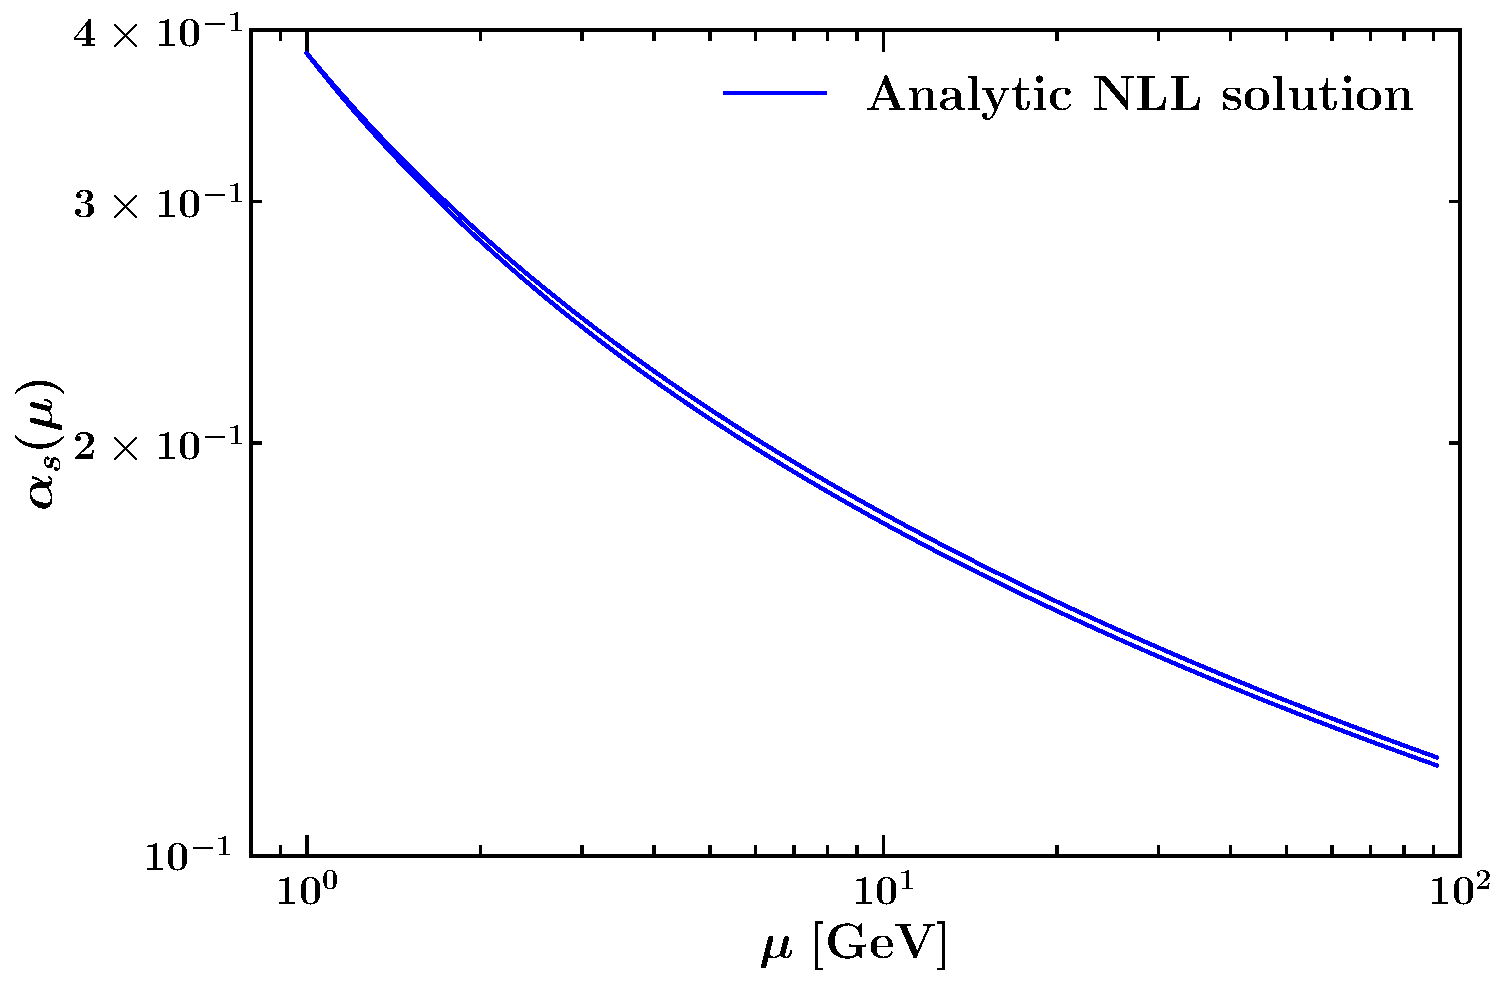
\includegraphics[width=0.6\textwidth]{plots/Alphas.pdf}
    \caption{Non-conservativity of the NLL analytic evolution of the
      strong coupling.\label{fig:Alphas}}
  \end{centering}
\end{figure}

Of course, one can argue that this effect is subleading and thus
allowed. On the other hand, one may wonder whether a violation of the
evolution equation introduced with the sole purpose of obtaining an
analytic expression for the evolution is justified. In fact, it
appears to be a better practice to employ an evolution that obeys the
evolution equation exactly order by order in perturbation theory. The
reason is simply a better control on the theoretical uncertainty
related to missing higher-order corrections. To be more specific, the
subleading terms introduced to obtain Eq.~(\ref{eq:ansolut}) would
affect the computation of an observable at fixed-order in perturbation
theory in the exact same way as a renormalisation scale variation
would do. Therefore, it appears more transparent to use an exact
solution to the evolution equation and leave the estimate of
theoretical uncertainties to renormalisation-scale variations.

\subsection{DGLAP evolution}

As a second application of Eq.~(\ref{eq:RGEproto}), we consider the
DGLAP evolution in which the quantity $R$ is identified with a
collinear distribution $f$. In order to simplify the discussion, we
consider the Mellin moments of a non-singlet distribution whose
evolution equation can be written as exactly as in
Eq.~(\ref{eq:RGEproto}) with $R=f$ and $\gamma$ the appropriate
anomalous dimension. Our aim is to find a solution to this equation in
perturbation theory by computing $f$ at some final scale $\mu$ when
knowing $f$ at some initial scale $\mu_0$. Of course, the solution to
the evolution equation is:
\begin{equation}
\begin{array}{rcl}
f(\mu)&=&\displaystyle
\exp\left[\int_{\mu_0}^{\mu}d\ln\mu'\,\gamma(a_s(\mu'))\right]f(\mu_0)\\
\\
&=&\displaystyle
    \exp\left[\sum_{n=0}^k\gamma^{(n)}\int_{\mu_0}^{\mu}d\ln\mu'\,a_s^{n+1}(\mu')\right]f(\mu_0)\\
\\
&=&\displaystyle f(\mu_0) \prod_{n=0}^k\exp\left[\gamma^{(n)}I_n\right]f(\mu_0)\,,
\end{array}
\label{eq:dglapsol}
\end{equation}
with:
\begin{equation}
I_n=\int_{a_s(\mu_0)}^{a_s(\mu)}da_s\left(\frac{a_s^{n}}{\overline{\beta}(a_s)}\right)\,.
\end{equation}
In the second line of Eq.~(\ref{eq:dglapsol}) we have used the
perturbative expansion of the anomalous dimension $\gamma$ and in the
third line made a change of variable in the integral using
Eq.~(\ref{eq:RGEalphas}). It is now opportune to analyse the integrals
$I_n$. The first question that we ask is whether the perturbative
expansion of $\gamma$ and $\overline{\beta}$ are related. More
specifically, given a $k+1$ terms in the expansion of
$\overline{\beta}$, is there any bound on the number of terms in the
expansion of $\gamma$ in terms of logarithmic accuracy? In order to
answer this question, it is necessary to first understand what kind of
logarithms Eq.~(\ref{eq:dglapsol}) is actually resumming. Indeed, one
may wonder whether the evolution of $\alpha_s$ alone is enough to
rusum all the large logarithms. If so, we would be enabled to expand
and truncate the exponential to the desired perturbative accuracy
because higher orders would be suppressed by powers of $\alpha_s$. The
answer to this question boils down to determining whether $I_n$ is
logarithmically enhanced for some value of $n$. We assume that
$\overline\beta$ is truncated at some power $k'+1$, with $k'$
generally different from $k$ in Eq.~(\ref{eq:dglapsol}). To give a
quantitative argument let us take $k'=2$, such that
\begin{equation}
\overline{\beta}(a_s) =\beta^{(0)}a_s\left[1+b_1a_s\right]\,.
\end{equation}
We then compute $I_0$, $I_1$, and $I_2$:
\begin{equation}
\begin{array}{rcl}
  I_0&=&\displaystyle\frac1{\beta^{(0)}}\int_{a_s(\mu_0)}^{a_s(\mu)}da_s\left(\frac{1}{a_s+b_1a_s^2}\right)=\frac1{\beta^{(0)}}\left[\ln
         a_s-\ln(1+b_1a_s)\right]\bigg|_{a_s(\mu_0)}^{a_s(\mu)}=\frac{1}{\beta^{(0)}}\ln\left(\frac{a_s(\mu)}{a_s(\mu_0)}\right)+\mathcal{O}(a_s)\,,\\
\\
  I_1&=&\displaystyle \frac1{\beta^{(0)}}\int_{a_s(\mu_0)}^{a_s(\mu)}da_s\left(\frac{1}{1+b_1a_s}\right)=\frac1{\beta^{(0)}}\left[\frac{\ln(1+b_1a_s)}{b_1}\right]\bigg|_{a_s(\mu_0)}^{a_s(\mu)}=\mathcal{O}(a_s) \,,\\
\\
  I_2&=&\displaystyle\frac1{\beta^{(0)}}\int_{a_s(\mu_0)}^{a_s(\mu)}da_s\left(\frac{a_s}{1+b_1a_s}\right)=\frac1{\beta^{(0)}}\left[\frac{a_s}{b_1}-\frac{\ln(1+b_1a_s)}{b_1^2}\right]\bigg|_{a_s(\mu_0)}^{a_s(\mu)}=\mathcal{O}(a_s^2)\,.
\end{array}
\label{eq:intsI}
\end{equation}
In general one finds that, for $n\geq1$,
$I_n=\mathcal{O}(a_s^n)$. Therefore, the exponential in
Eq.~(\ref{eq:dglapsol}) can  safely be expanded:
\begin{equation}
\exp\left[\gamma^{(n)}I_n\right]=1+\gamma^{((n))}\times\mathcal{O}(a_s^n)\,,\quad n\geq 1\,.
\end{equation}
Somewhat surprisingly, this reveals that the inclusion of perturbative
corrections beyond leading order to the anomalous dimension $\gamma$
does not directly improve the logarithmic accuracy of the resummation
provided by the evolution. The exception to this pattern is $I_0$ that
cannot be (fully) expanded due to the presence of a logarithm of
$a_s(\mu)/a_s(\mu_0)$ that, as can be see from Eq.~(\ref{eq:llsol}),
is potentially large:
\begin{equation}
\exp\left[\gamma^{(0)}I_0\right]=\exp
\left[\frac{\gamma^{(0)}}{\beta^{(0)}}\ln\left(\frac{a_s(\mu)}{a_s(\mu_0)}\right)\right]+\mathcal{O}(a_s)=\left(\frac{a_s(\mu)}{a_s(\mu_0)}\right)^{\frac{\gamma^{(0)}}{\beta^{(0)}}}+\mathcal{O}(a_s)\,.
\label{eq:expres}
\end{equation}
This factor alone provides the resummation up to some logarithmic
accuracy determined uniquely by the evolution of $a_s(\mu)$. Finally
one has:
\begin{equation}
f(\mu) = \displaystyle
\left[1+\mathcal{O}(a_s)\right]\left(\frac{a_s(\mu)}{a_s(\mu_0)}\right)^{\frac{\gamma^{(0)}}{\beta^{(0)}}}f(\mu_0)
\,.
\label{eq:dglapanal}
\end{equation}
However, the inclusion of correction terms in the square brackets in
the r.h.s. of Eq.~(\ref{eq:dglapanal}) is still required to attain
some given logarithmic accuracy. Since the exponential in
Eq.~(\ref{eq:expres}) resums single logarithms of the kind
$a_s^m\ln ^m(\mu/\mu_0)$, a term proportional to $a_s^n$ (without any
logarithm) belongs to the tower $a_s^{m+n}\ln ^m(\mu/\mu_0)$ and thus
contributes to N$^n$LL. To make an example, suppose we want to achieve
NLL resummation. To do so, we need to include the $\mathcal{O}(a_s)$
in the squared bracket of Eq.~(\ref{eq:dglapanal}) because that
contributes to NLL. That term can be easily computed by retaining the
$\mathcal{O}(a_s)$ terms in Eq.~(\ref{eq:intsI}). Moreover, $a_s(\mu)$
in the last factor has to be computed using the NLL evolution given
in Eq.~(\ref{eq:ansolNLL}). This finally gives:
\begin{equation}
f^{\rm NLL}(\mu) = \displaystyle\left[1+\frac1{\beta^{(0)}}\left(\gamma^{(1)}-b_1
    \gamma^{(0)}\right) \left(a_s^{\rm LL}(\mu)-a_s(\mu_0)\right)\right]
\left(\frac{a_s^{\rm NLL}(\mu)}{a_s(\mu_0)}\right)^{\frac{\gamma^{(0)}}{\beta^{(0)}}} f(\mu_0) \,.
\end{equation}
Also note that in the squared bracket we are entitled to replaced
$a_s$ with $a_s^{\rm LL}$ becase the difference is
$\mathcal{O}(a_s^2)$ and thus NNLL.

In order to make a step towards the notation typically used in $q_T$
resummation, we introduce the quantity:
\begin{equation}
\lambda \equiv \lambda(\mu) =
a_s(\mu_0)\beta^{(0)}\ln\left(\frac{\mu}{\mu_0}\right)\,,
\label{eq:lambdadef}
\end{equation}
that allows us to write the LL and NLL RGE solution for $a_s$ as:
\begin{equation}
a_s^{\rm LL}(\mu) = a_s(\mu_0)\frac{1}{1-\lambda}\,,
\end{equation}
and:
\begin{equation}
a_s^{\rm NLL}(\mu)=a_s(\mu_0)\frac{1}{1-\lambda}\left[1 - a_s(\mu_0) \frac{b_1 \ln\left(1-\lambda\right)}{1-\lambda}\right]\,,
\end{equation}
such that:
\begin{equation}
\begin{array}{rcl}
  f^{\rm NLL}(\mu) &=&\displaystyle \displaystyle \left[1+a_s(\mu_0)\frac1{\beta^{(0)}}\left(\gamma^{(1)}-b_1
                            \gamma^{(0)}\right)
                            \frac{\lambda}{1-\lambda}\right]\\
  \\
                   &\times&\displaystyle                        \exp\left[-\frac{\gamma^{(0)}}{\beta^{(0)}}\ln\left(1-\lambda\right)-a_s(\mu_0) \frac{\gamma^{(0)}b_1}{\beta^{(0)}}\frac{
                       \ln\left(1-\lambda\right)}{1-\lambda}\right]f(\mu_0)\,.
\end{array}
\end{equation}
We now introduce the functions:
\begin{equation}
\begin{array}{rcl}
g^{(0)}(\lambda) &=& \displaystyle  1+a_s(\mu_0)\frac1{\beta^{(0)}}\left(\gamma^{(1)}-b_1
                            \gamma^{(0)}\right)
                            \frac{\lambda}{1-\lambda}\,,\\
\\
g^{(1)}(\lambda) &=& \displaystyle
                     -\frac{\gamma^{(0)}}{\beta^{(0)}}\ln\left(1-\lambda\right)\,,\\
\\
g^{(2)}(\lambda) &=& \displaystyle -\frac{\gamma^{(0)}b_1}{\beta^{(0)}}\frac{
                       \ln\left(1-\lambda\right)}{1-\lambda}\,,
\end{array}
\end{equation}
such that:
\begin{equation}
  f^{\rm NLL}(\mu) =
  g^{(0)}(\lambda)\exp\left[g^{(1)}(\lambda)+a_s(\mu_0)
    g^{(2)}(\lambda)\right]f(\mu_0) \,.
\label{eq:DGLAPalaSoftGlue}
\end{equation}
This procedure can be extended to N$^k$LL accuracy just by introducing
the appropriate $g^{(n)}$ functions, with $n\leq k+1$, in the
exponential and including corrections up to $\mathcal{O}(a_s^k)$ in
$g^{(0)}$. The notation is purposely reminiscent of soft-gluon and
$q_T$ resummation.

We can use the parallel with soft-gluon resummation to introduce
the analogous of a ``resummation'' scale. This is done by introducing
an \textit{arbitrary} scale $\mu_{\rm R}\sim \mu_0$ along with the
trivial equality:
\begin{equation}
\ln\left(\frac{\mu}{\mu_0}\right) = \ln\left(\frac{\mu}{\mu_{\rm R}}\right)
+ \ln\left(\frac{\mu_{\rm R}}{\mu_0}\right)\,,
\end{equation}
such that $\ln\left(\mu_{\rm R}/\mu_0\right)\sim 1$. Using
Eq.~(\ref{eq:lambdadef}), one has:
\begin{equation}
  \lambda =
  a_s(\mu_0)\beta^{(0)}\ln\left(\frac{\mu}{\mu_{\rm R}}\right)+a_s(\mu_0)\beta^{(0)}\ln\left(\frac{\mu_{\rm
        R}}{\mu_0}\right)=\overline{\lambda}+a_s(\mu_0)\beta^{(0)}\ln\left(\frac{\mu_{\rm
        R}}{\mu_0}\right)\,,
\end{equation}
where the second term in the r.h.s. is not enhanced by a large
logarithm and can thus be treated perturbatively. Writing the
functions $g^{(n)}$ in terms of $\overline{\lambda}$ and neglecting
subleading terms gives the new functions:
\begin{equation}
\begin{array}{rcl}
\overline{g}^{(0)}(\overline{\lambda}) &=& \displaystyle  1+a_s(\mu_0)\frac1{\beta^{(0)}}\left(\gamma^{(1)}-b_1
                            \gamma^{(0)}\right)
                            \frac{\overline{\lambda}}{1-\overline{\lambda}}\,,\\
\\
\overline{g}^{(1)}(\overline{\lambda}) &=& \displaystyle
                     -\frac{\gamma^{(0)}}{\beta^{(0)}}\ln\left(1-\overline{\lambda}\right)\,,\\
\\
\overline{g}^{(2)}(\overline{\lambda}) &=& \displaystyle -\frac{\gamma^{(0)}}{1-\overline{\lambda}}\left[\frac{b_1}{\beta^{(0)}}\ln\left(1-\overline{\lambda}\right)-\ln\left(\frac{\mu_{\rm
        R}}{\mu_0}\right)\right]\,,
\end{array}
\end{equation}
so that:
\begin{equation}
  f^{\rm NLL}(\mu) =
  \overline{g}^{(0)}(\overline{\lambda})\exp\left[\overline{g}^{(1)}(\overline{\lambda})+a_s(\mu_0)
    \overline{g}^{(2)}(\overline{\lambda})\right]f(\mu_0) \,.
\label{eq:DGLAPalaSoftGlueMuR}
\end{equation}
Eqs.~(\ref{eq:DGLAPalaSoftGlueMuR}) and~(\ref{eq:DGLAPalaSoftGlue})
are both NLL accurate and only differ by subleading terms. In fact,
Eq.~(\ref{eq:DGLAPalaSoftGlueMuR}) generalises
Eq.~(\ref{eq:DGLAPalaSoftGlue}) because the latter reduces to the
former for $\mu_{\rm R}=\mu_0$. Therefore, one should be able to use
modest variations of $\mu_{\rm R}$ around $\mu_0$ to estimate the
possible impact of higher-order corrections to the anomalous
dimension.

Eq.~(\ref{eq:DGLAPalaSoftGlueMuR}) provides a closed-form, fully
analytical solution to the RGE, Eq.~(\ref{eq:RGEproto}), for collinear
distributions. However, exactly like in the case of the analytical
solution for $a_s$, Eq.~(\ref{eq:dglapanal}) will satisfy
Eq.~(\ref{eq:RGEproto}) only up to subleading terms with a consequent
non-conservative pattern of the evolution. Conversely, a numerical
evaluation of the solution in Eq.~(\ref{eq:dglapsol}) will obey
exactly Eq.~(\ref{eq:RGEproto}) and the evolution will be
conservative.

\subsection{The Sudakov form factor}

Now, we turn to address the question of solving the TMD evolution
equations in Eq.~(\ref{eq:eveqs}) in perturbation theory. We have
already derived the solution, Eq.~(\ref{eq:solution2}), in terms of
the relevant anomalous dimensions. However, this solution contains an
integral. A possibility is that of computing that integral
numerically. This ensures that the results obeys \textit{exactly} the
evolution equations in Eq.~(\ref{eq:eveqs}) and the evolution is
conservative. Another possibility is that of attempting to solve the
integral analytically. This turns out to be possible provided that one
uses the appropriate analytic solution for the running of
$a_s$. As discussed above, this comes at the price that the
result violates the equations in Eq.~(\ref{eq:eveqs}) by subleading
terms. As we will see below, this very violation gives origin to the
resummation scale.

In order to derive a fully analytic expression for the expression in
Eq.~(\ref{eq:solution2}) we need to consider the perturbative
expansion of the relevant anomalous dimensions. This is done in
Eq.~(\ref{eq:Sudexp}) for the square of the evolution operator that is
relevant to Drell-Yan production. In order to match the notation of
this section. we identify $\mu_b=\mu$ and $Q=\mu_0$ in
Eq.~(\ref{eq:Sudexp}). In addition, we limit ourselves to consider the
NNLL accuracy that means truncating the expansion at $n=2$ for
$\gamma_K$ and at $n=1$ for $K$ and $\gamma_F$. This finally gives:
\begin{equation}
\begin{array}{rcl}
  R^{\rm NNLL} &=&\displaystyle  \exp\bigg\{-\sum_{n=0}^1 K^{(n,0)}
        \left[a_s^{{\rm N}^{1-n}{\rm
        LL}}(\mu)\right]^{n+1}\ln\frac{\mu}{\mu_0}-\sum_{n=0}^1
        \gamma_F^{(n)}\int_{\mu_0}^{\mu}\frac{d\mu'}{\mu'}\left[a_s^{{\rm
        N}^{1-n}{\rm LL}}(\mu')\right]^{n+1}\\
\\
 &-&\displaystyle \sum_{n=0}^2
     \gamma_K^{(n)}\int_{\mu_0}^{\mu}\frac{d\mu'}{\mu'}\left[a_s^{{\rm
     N}^{2-n}{\rm
     LL}}(\mu')\right]^{n+1}\ln\frac{\mu'}{\mu_0}\bigg\}\,,
\end{array}
\end{equation}
where we have also used the fact that:
\begin{equation}
a_s = a_s^{{\rm N}^{k}{\rm LL}}\left[1+\mathcal{O}(a_s^k)\right]\,.
\end{equation}
It is convenient to express the above equation in terms of the
variable $\lambda$ defined in Eq.~(\ref{eq:lambdadef}). This leads to:
\begin{equation}
\begin{array}{rcl}
  R^{\rm NNLL} &=&\displaystyle  \exp\Bigg\{-\frac{1}{\beta^{(0)}a_s(\mu_0)}\sum_{n=0}^1\left( K^{(n,0)}
        \lambda\left[a_s^{{\rm N}^{1-n}{\rm
        LL}}(\lambda)\right]^{n+1}+
        \gamma_F^{(n)}\int_{0}^{\lambda}d\lambda'\left[a_s^{{\rm
        N}^{1-n}{\rm LL}}(\lambda')\right]^{n+1}\right)\\
\\
 &-&\displaystyle \left(\frac{1}{\beta^{(0)}a_s(\mu_0)}\right)^2\sum_{n=0}^2
     \gamma_K^{(n)}\int_{0}^{\lambda}d\lambda'\,\lambda'\left[a_s^{{\rm
     N}^{2-n}{\rm
     LL}}(\lambda')\right]^{n+1}\Bigg\}\,,
\end{array}
\end{equation}
where $\lambda'=\lambda(\mu')$ and $a_s(\lambda)\equiv a_s(\mu)$. We
write it more explicitly as:
\begin{equation}
\begin{array}{rcl}
  R^{\rm NNLL} &=&\displaystyle  \exp\Bigg\{-\frac{1}{\beta^{(0)}a_s(\mu_0)}\left( K^{(0,0)}
        \lambda a_s^{{\rm NLL}}(\lambda)+
        \gamma_F^{(0)}\int_{0}^{\lambda}d\lambda' a_s^{{\rm NLL}}(\lambda')+ K^{(1,0)}
        \lambda\left[a_s^{{\rm
        LL}}(\lambda)\right]^{2}+
        \gamma_F^{(1)}\int_{0}^{\lambda}d\lambda'\left[a_s^{{\rm LL}}(\lambda')\right]^{2}\right)\\
\\
 &-&\displaystyle \left(\frac{1}{\beta^{(0)}a_s(\mu_0)}\right)^2\left(
     \gamma_K^{(0)}\int_{0}^{\lambda}d\lambda'\,\lambda' a_s^{{\rm
     NNLL}}(\lambda')+\gamma_K^{(1)}\int_{0}^{\lambda}d\lambda'\,\lambda'\left[a_s^{{\rm
     NLL}}(\lambda')\right]^{2}+\gamma_K^{(2)}\int_{0}^{\lambda}d\lambda'\,\lambda'\left[a_s^{{\rm
     LL}}(\lambda')\right]^{3}\right)\Bigg\}\,.
\end{array}
\end{equation}
We now need to compute the integrals involving the strong coupling
$a_s$. This can be done using the analytic expressions derived in
Sect.~\ref{sec:strongcoupling}.The task is simplified by the fact that
$a_s^{{\rm N}^k{\rm LL}}$, for $k>0$, can be written in terms of
$a_s^{\rm LL}$ (see Eqs.~(\ref{eq:ansolut}) and
(\ref{eq:ansolutnnll})) so that we can exploit the relations:
\begin{equation}
\int_0^\lambda d\lambda'\,f\left(a_s^{\rm LL}(\lambda')\right) =
a_s(\mu_0)\int_{a_s(\mu_0)}^{a_s^{\rm LL}(\lambda)}\frac{da}{a^2}\,f(a)\,,
\end{equation}
\begin{equation}
\int_0^\lambda d\lambda'\,\lambda'\,f\left(a_s^{\rm LL}(\lambda')\right) =
\int_0^\lambda d\lambda'\,f\left(a_s^{\rm LL}(\lambda')\right)-a_s^2(\mu_0)\int_{a_s(\mu_0)}^{a_s^{\rm LL}(\lambda)}\frac{da}{a^3}\,f(a)\,.
\end{equation}

\section{Iterative solution of the strong coupling running}

In this section, I will derive a general formula to compute
iteratively the running of the strong coupling. In order to simplify
the notation, I will refer to the strong coupling computed at some
generic scale as to $a$, while I will call $a_0$ the value of coupling
at the reference scale. The corresponding RGE will then be:
\begin{equation}
\frac{d\ln a}{d\ln \mu} = \beta(a)\,,
\label{eq:allorders}
\end{equation}
with:
\begin{equation}
\beta(a) = a\sum_{n=0}^\infty \beta_n a^n\,.
\end{equation}
If one truncates the $\beta$ function at the first order, the
resulting evolution equation reads:
\begin{equation}
\frac{d\ln a_{\rm LL}}{d\ln \mu} = a_{\rm LL}\beta_0\,,
\end{equation}
that admits a simple closed-form exact solution:
\begin{equation}
a_{\rm LL}(\mu) =
\frac{a_0}{1-a_0\beta_0\ln\left(\frac{\mu}{\mu_0}\right) }\,.
\label{eq:leadingorder}
\end{equation}
Since we know how to write $a_{\rm LL}$ in a closed form, we can
combine Eqs.~(\ref{eq:allorders}) and~(\ref{eq:leadingorder}) as
follows:
\begin{equation}
\frac{d\ln a}{d\ln a_{\rm LL}} =\frac{a}{a_{\rm LL}}\sum_{n=0}^\infty b_na^n\,,\quad\mbox{with}\quad b_n=\frac{\beta_n}{\beta_0}\,.
\end{equation}
Now we can attempt to solve this equation whose general solution is:
\begin{equation}
\int_{a_0}^{a_{\rm
    LL}}\frac{dy}{y^2}=\int_{a_0}^{a}\frac{dx}{x^2}\left(\sum_{n=0}^\infty
  b_nx^n\right)^{-1}\,.
\label{eq:intrun}
\end{equation}
Assuming that $x\ll 1$ (as it should be in the perturbative regime),
one can write:
\begin{equation}
\left(\sum_{n=0}^\infty b_nx^n\right)^{-1}=\sum_{n=0}^\infty \overline{b}_nx^n\,,
\end{equation}
where the coefficients $\overline{b}_n$ can be iteratively determined
in terms of the coefficients ${b}_n$. The terms up to $x^3$ read:
\begin{equation}
\begin{array}{rcl}
\overline{b}_1  &=& - b_1\,,\\
\overline{b}_2  &=& - b_2+b_1^2\,,\\
\overline{b}_3  &=& - b_3+2b_2b_1-b_1^3\,.
\end{array}
\end{equation}
Plugging this expansion into Eq.~(\ref{eq:intrun}) and solving the
integrals gives:
\begin{equation}
\frac{1}{a_{\rm LL}} = \frac{1}{a}-\overline{b}_1\ln\left(\frac{a}{a_0}\right)-\sum_{k=1}^\infty\frac{\overline{b}_{k+1}}{k}\left(a^k-a_0^k\right)\,.
\end{equation}
This is a transcendental equation in $a$ that can be solved
iteratively assuming that $a,a_0\ll 1$. Upon this assumption, the
terms in the r.h.s. of the equation above are increasingly
smaller. Therefore, at the first order one has:
\begin{equation}
\frac{1}{a_{\rm LL}} = \frac{1}{a}\quad\Longrightarrow\quad a = a_{\rm
LL}\,,
\end{equation}
as expected. At second order instead:
\begin{equation}
\frac{1}{a_{\rm LL}} = \frac{1}{a}-\overline{b}_1\ln\left(\frac{a}{a_0}\right)\,.
\end{equation}
This is a transcendental equation that can be solved by observing that
the second term in the r.h.s. is subleading w.r.t. the first and thus
one can plug into that term the first order solution, that is:
\begin{equation}
\frac{1}{a_{\rm LL}} = \frac{1}{a}-\overline{b}_1\ln\left(\frac{a_{\rm
    LL}}{a_0}\right)\,.
\end{equation}
This equation can now be resolved for $a$ obtaining:
\begin{equation}
  a = a_{\rm NLL}=\frac{a_{\rm LL}}{\displaystyle 1+a_{\rm LL}\overline{b}_1\ln\left(\frac{a_{\rm
          LL}}{a_0}\right)}\,.
\end{equation}
One can keep iterating in the same way finally obtaining the general
recursive formula for the analytic N$^{n}$LL solution:
\begin{equation}
a_{{\rm N}^{n}{\rm LL}}=a_{\rm LL}\left\{1+a_{\rm LL}\left[\overline{b}_1\ln\left(\frac{a_{{\rm
          N}^{n-1}{\rm LL}}}{a_0}\right)+\sum_{k=1}^{n-1}\frac{\overline{b}_{k+1}}{k}\left(a_{{\rm
          N}^{n-k-1}{\rm
          LL}}^k-a_0^k\right)\right]\right\}^{-1}+\mathcal{O}(a^{n+2})\,,\quad
n\geq 1\,.
\label{eq:masterf}
\end{equation}
Note also that the curly bracket, that appears in the denominator, can
be further expanded and truncated to the relevant order because the
single terms appearing there are increasingly subleading.

At this stage it is important to highlight a feature of the analytic
solution of running of the strong coupling. Due to its iterative
nature, the N$^{n}$LL solution will only depend on $a_{\rm LL}$. This
allows us to write the solution to all other RGEs, such as the DGLAP
evolution equations and the Collins-Soper equation, in terms of
$a_{\rm LL}$ only.

Additionally, it is interesting to observe that there are \textit{two}
resummation structures. The first is contained in $a_{\rm LL}$ and
given by the geometric summation in Eq.~(\ref{eq:leadingorder}). The
second is $\ln\left(\frac{a_{{\rm N}^{n-1}{\rm
        LL}}}{a_0}\right)$. This structure first appears at NLL as:
\begin{equation}
a_{{\rm NLL}}=a_{\rm LL}\left[1+a_{\rm LL}\overline{b}_1\ln\left(\frac{a_{\rm LL}}{a_0}\right)\right]^{-1}+\mathcal{O}(a^3)=a_{\rm LL}\left[1-a_{\rm LL}\overline{b}_1\ln\left(\frac{a_{\rm LL}}{a_0}\right)\right]+\mathcal{O}(a^3)\,.
\end{equation}
When going further, the content of the logarithm will be the coupling
computed at higher logarithmic orders. However, beyond LL, the
logarithm can be expanded around $a_{\rm LL}=0$ finally leading to
$\ln\left(\frac{a_{\rm LL}}{a_0}\right)$. As an example, we consider
$a_{\rm NNLL}$ that, using Eq.~(\ref{eq:masterf}), reads:
\begin{equation}
\begin{array}{rcl}
  a_{\rm NNLL}&=&\displaystyle a_{\rm LL}\left\{1+a_{\rm
                  LL}\left[\overline{b}_1\ln\left(\frac{a_{\rm NLL}}{a_0}\right)+\overline{b}_{2}\left(a_{\rm
                  LL}-a_0\right)\right]\right\}^{-1}+\mathcal{O}(a^4)\\
  \\
              &=&\displaystyle a_{\rm LL}\left\{1-a_{\rm LL}\left[\overline{b}_1 \ln\left(\frac{a_{\rm
                  LL}}{a_0}\right)+\overline{b}_{2}\left(a_{\rm
                  LL}-a_0\right) \right]+a_{\rm
                  LL}^2 \overline{b}_1^2\ln\left(\frac{a_{\rm LL}}{a_0}\right)\left(1+\ln\left(\frac{a_{\rm LL}}{a_0}\right)\right)\right\}+\mathcal{O}(a^4)\,.
\end{array}
\end{equation}

\section{Analytic calculation of the Collins-Soper kernel}

In this section, we compute analytically to different logarithmic
accuracies the solution of the Collins-Soper evolution equation
Eq.~(\ref{eq:CuspRGE}). This amounts to computing
Eq.~(\ref{eq:CuspEv}) plugging in the appropriate perturbative
corrections. To do so, we choose as an initial scale
$\mu_0=\mu_b=2e^{-\gamma_E}/b_T$ that is such that the expansion of
$K$ at this scale admits a log-free perturbative expansion (see
Eq.~(\ref{eq:Kexp})). Therefore, the integral to be computed is:
\begin{equation}
K(\mu) = K(\mu_b) -
\int_{\mu_b}^{\mu}\frac{d\mu'}{\mu'}\gamma_K(\alpha_s(\mu'))\,,
\end{equation}
that upon expansion of the $K$ and $\gamma_K$ anomalous dimensions
becomes:
\begin{equation}
K(\mu) = 
\sum_{n=0}^{\infty}a_s^{n+1}(\mu_b)K^{(n,0)}- \sum_{n=0}^{\infty}\gamma_K^{(n)} 
\int_{\mu_b}^{\mu}\frac{d\mu'}{\mu'} a_s^{n+1}(\mu')\,.
\end{equation}
Following the usual counting, to N$^k$LL accuracy the truncation of
the perturbative series is:
\begin{equation}
K(\mu) = 
\sum_{n=0}^{k-1}a_s^{n+1}(\mu_b)K^{(n,0)}- \sum_{n=0}^{k}\gamma_K^{(n)} 
\int_{\mu_b}^{\mu}\frac{d\mu'}{\mu'} a_s^{n+1}(\mu')\,,
\end{equation}
such that at LL one has:
\begin{equation}
K_{\rm LL}(\mu) =  - \gamma_K^{(0)}
\int_{\mu_b}^{\mu}\frac{d\mu'}{\mu'} a_s(\mu')\,,
\label{eq:KatLL}
\end{equation}
at NLL:
\begin{equation}
  K_{\rm NLL}(\mu) = 
  a_s(\mu_b)K^{(0,0)}- \gamma_K^{(0)} 
  \int_{\mu_b}^{\mu}\frac{d\mu'}{\mu'} a_s(\mu')-\gamma_K^{(1)} 
  \int_{\mu_b}^{\mu}\frac{d\mu'}{\mu'} a_s^{2}(\mu')\,,
\label{eq:KatNLL}
\end{equation}
at NNLL:
\begin{equation}
K_{\rm NNLL}(\mu) = 
  a_s(\mu_b)K^{(0,0)}+a_s^2(\mu_b)K^{(1,0)}- \gamma_K^{(0)} 
  \int_{\mu_b}^{\mu}\frac{d\mu'}{\mu'} a_s(\mu')-\gamma_K^{(1)} 
  \int_{\mu_b}^{\mu}\frac{d\mu'}{\mu'} a_s^{2}(\mu') -\gamma_K^{(2)} 
  \int_{\mu_b}^{\mu}\frac{d\mu'}{\mu'} a_s^{3}(\mu')\,,
\label{eq:KatNNLL}
\end{equation}
and so on. The question now boils down to computing analytically the
integrals of different powers of $a_s$. To do so, we need to use the
analytic solution of the running of the strong coupling. This can be
done by using the $g$-function approach developed in
Ref.~\cite{Bertone:2022sso} that is such that, using $a_s(\mu_b)$ as
boundary condition, the N$^k$LL evolution reads:
\begin{equation}
a_s^{{\rm N}^{k}{\rm LL}}(\mu') = a_s(\mu_b)\sum_{l=0}^{k}a_s^l(\mu_b) g_{l+1}^{(\beta)}(\lambda)\,,
\end{equation}
with the $g$-functions relevant up to NNLL given by:
\begin{equation}
\begin{array}{rcl}
g_1^{(\beta)}(\lambda)&=&\displaystyle \frac{1}{1-\lambda}\,,\\
\\
g_2^{(\beta)}(\lambda)&=&\displaystyle -\frac{b_1\ln(1-\lambda)}{(1-\lambda)^2}\,,\\
\\
g_3^{(\beta)}(\lambda)&=&\displaystyle \frac{b_2\lambda-b_1^2\left(\lambda+\ln\left(1-\lambda\right)-\ln^2\left(1-\lambda\right)\right)}{(1-\lambda)^3} \,,\\
\end{array}
\end{equation}
where:
\begin{equation}
  \lambda = a_s(\mu_b)\beta^{(0)}\ln\left(\frac{\mu'}{\mu_b}\right)\,,
\end{equation}
and $b_n=\beta^{(n)}/\beta^{(0)}$. Since the integration variable only
appears through $\lambda$, it is convenient to make a change of
variable and, with a little abuse of notation, rewrite the integrals
as follows:
\begin{equation}
\int_{\mu_b}^{\mu}\frac{d\mu'}{\mu'} a_s^{p}(\mu') =
\frac{1}{a_s(\mu_b)\beta^{(0)}}\int_0^{\lambda_\mu} d\lambda\,a_s^{p}(\lambda)\,,
\end{equation}
with:
\begin{equation}
  \lambda_\mu = a_s(\mu_b)\beta^{(0)}\ln\left(\frac{\mu}{\mu_b}\right)\,.
\end{equation}
At LL, we can plug the LL solution of the strong coupling into
Eq.~(\ref{eq:KatLL}) producing:
\begin{equation}
K_{\rm LL}(\mu) =\frac{\gamma_K^{(0)}}{\beta^{(0)}}\ln(1-\lambda_\mu)\,.
\end{equation}
At NLL, we plug the NLL solution of the strong coupling into the first
integral of Eq.~(\ref{eq:KatNLL}) and the LL solution into the second
integral finding:
\begin{equation}
  K_{\rm NLL}(\mu) =K_{\rm LL}(\mu)+
  a_s(\mu_b)\left[K^{(0,0)} + \frac{b_1\gamma_K^{(0)}}{\beta^{(0)}}\frac{\lambda_\mu+\ln(1-\lambda_\mu)}{1-\lambda_\mu}-
  \frac{\gamma_K^{(1)}}{\beta^{(0)}}\frac{\lambda_\mu}{1-\lambda_\mu}\right]\,.
\end{equation}
At NNLL, following the same pattern, we find:
\begin{equation}
\begin{array}{rcl}
  K_{\rm NNLL}(\mu) &=& K_{\rm NLL}(\mu)\\
\\
&+&\displaystyle
  a_s^2(\mu_b)\bigg[K^{(1,0)} 
- \frac{b_2\gamma_K^{(0)}}{\beta^{(0)}}\frac{\lambda_\mu^2}{2(1-\lambda_\mu)^2}
+ \frac{b_1^2\gamma_K^{(0)}}{\beta^{(0)}}\frac{\lambda_\mu^2-\ln^2(1-\lambda_\mu)}{2(1-\lambda_\mu)^2}\\
\\
&+&\displaystyle
    \frac{b_1\gamma_K^{(1)}}{\beta^{(0)}}\frac{2\ln(1-\lambda_\mu)-\lambda_\mu(\lambda_\mu-2)}{2(1-\lambda_\mu)^2}+
\frac{\gamma_K^{(2)}}{\beta^{(0)}} \frac{\lambda_\mu(\lambda_\mu-2)}{2(1-\lambda_\mu)^2}
\bigg]\,.
\end{array}
\end{equation}
It is clear that to N$^k$LL this generalises to:
\begin{equation}
  K_{{\rm N}^k{\rm LL}}(\mu) = \sum_{n=0}^k a_s^n(\mu_b)g_{n}^{(K)}(\lambda_\mu)\,,
\end{equation}
where the appropriate $g$-functions up to NNLL can be read off from
the calculations above.

\section{Analytic perturbation theory}

The fact highlighted above that the solution to all other RGEs
relevant to resum large logarithms of $q_T$ can be written in terms of
$a_{\rm LL}$ only is particularly relevant. As a matter of fact, this
will eventually allow us to eliminate the Landau pole simply by
requiring that $a_{\rm LL}$, or equivalently the one-loop
$\beta$-function, has the correct analytic structure in the complex
$\mu$ plane. This approach is often referred to analytic perturbation
theory (APT) and was originally suggested by Bogolyubov, Logiunov, and
Shirkov back in 1959~\cite{Bogolyubov:1960cha} to obtain the correct
causality properties of the QED Green's functions also when working at
fixed-order in perturbation theory. At one-loop order, this boils down
to requiring that the strong coupling $a_{\rm LL}$ admits a spectral
representation allowing to restore the analytic properties of the
two-point Green's function required for causality to be fulfilled. The
direct consequence of the procedure is the natural appearance of power
suppressed terms of the form $\Lambda/\mu$ that automatically
eliminate the Landau pole making the strong coupling $a_{\rm LL}$
finite for all values of $\mu$.

However, $a_{\rm LL}$ does not only appears as integer powers but also
within logs. It is therefore crucial to be able to treat these terms
correctly preserving the correct analytical structure on the complex
$\mu$. Here fractional analytical perturbation theory (FAPT) comes to
rescue~\cite{Bakulev:2005gw}.

\section{Derivation of analytic expression for g-functions in $q_{T}$-resummation}

\subsection{The Sudakov integral}
The Sudakov exponential has the following explicit form:

\begin{equation}
S=-\int_{b_{0}^{2}/{b^{2}}}^{Q^{2}} \frac{dq^{2}}{q^{2}}\left[A\left(\alpha_{s}\left(q^{2}\right)\right)\ln\frac{M^{2}}{q^{2}}+\tilde B \left(\alpha_{s}\left(q^{2}\right)\right)\right],
\end{equation}

where $M$ is the invariant mass of the final state, $Q$ is the resummation scale, and $A, \tilde B$ are power series in $\alpha_{s}\left(Q^{2}\right)$.

The $A$ function is completely determined by the cusp anomalous dimensions. 

The $\tilde B$ function contains the usual $B$ coefficients and two additional terms coming from PDF evolution and coefficient functions.

From the PDF evolution equations in Mellin space

\begin{eqnarray}
f_{a,N}\left(\mu_{F}^{2}\right)&=&\sum _{b} U_{ab,N}\left(\frac{b_{0}^{2}}{b^{2}},\mu _{F}^{2}\right) f_{b,N}\mu _{F}^{2}\\
\frac{dU_{ab,N}\left(\mu ^{2},\mu _{F}^{2}\right)}{d\ln\mu^{2}}&=&\sum _{c}\gamma _{ac,N}\left(\alpha _{s}\left(\mu^{2}\right)\right) U_{cb,N}\left(\mu ^{2},\mu _{F}^{2}\right)
\end{eqnarray}

one obtains (for a single species of partons) the solution

\begin{equation}
U_{N}\left(b_{0}^{2}/b^{2},\mu _{F}^{2}\right)=\exp\left\{-\int_{b_{0}^{2}/{b^{2}}}^{\mu_{F}^{2}} \frac{dq^{2}}{q^{2}} \gamma_{N}\left(\alpha_{s}\left(q^{2}\right)\right)\right\}
\end{equation}

Thus we have the first additional contribution to $B$ coefficients: $B\longrightarrow B + 2 \, \gamma_{N} \, \alpha_{s}$.

As for the coefficient functions (again, in Mellin space),we can use the following renormalisation-group identity:

\begin{equation}
C_{N}\left(\alpha_{s}\left(b_{0}^{2}/b^{2}\right)\right)=C_{N}\left(\alpha_{s}\left(M^{2}\right)\right)\exp\left\{-\int_{b_{0}^{2}/{b^{2}}}^{M^{2}} \frac{dq^{2}}{q^{2}} \beta\left(\alpha_{s}\left(q^{2}\right)\right)\frac{d\ln C_{N}\left(\alpha_{s}\left(q^{2}\right)\right)}{d\ln\alpha_{s}\left(q^{2}\right)}\right\}
\end{equation}

to derive the second additional contribution to $B$ coefficients: $B\longrightarrow B + 2 \, \beta\left(\alpha_{s}\right) \frac{d\ln C_{N}\left(\alpha_{s}\right)}{d\ln\alpha_{s}}$.

The $\tilde B$ function is thus given by

\begin{equation}
\tilde B = B + 2 \, \gamma_{N} \, \alpha_{s} + 2 \, \beta\left(\alpha_{s}\right) \frac{d\ln C_{N}\left(\alpha_{s}\right)}{d\ln\alpha_{s}}.
\end{equation}

With simple math and a change of the integration variable, we have

\begin{eqnarray}
S&=&-\int_{b_{0}^{2}/{b^{2}}}^{Q^{2}} \frac{dq^{2}}{q^{2}}\left[A\left(\alpha_{s}\left(q^{2}\right)\right)\left(\ln\frac{M^{2}}{Q^{2}}+\ln\frac{Q^{2}}{q^{2}}\right)+\tilde B \left(\alpha_{s}\left(q^{2}\right)\right)\right]\\
&=&-\int_{b_{0}^{2}/{b^{2}}}^{Q^{2}} \frac{dq^{2}}{q^{2}}\left[A\left(\alpha_{s}\left(q^{2}\right)\right)\ln\frac{Q^{2}}{q^{2}}+\bar B \left(\alpha_{s}\left(q^{2}\right)\right)\right]\\
&=&\int_{\lambda}^{0} \frac{dt}{\beta_{0}\alpha_{s}}\left[A\left(\alpha_{s}\left(t\right)\right)\frac{t}{\beta_{0}\alpha_{s}}+\bar B \left(\alpha_{s}\left(t\right)\right)\right],
\end{eqnarray}

where $\lambda=\beta_{0}\alpha_{s}\ln\left(Q^{2}b^{2}/b_{0}^{2}\right)=\beta_{0}\alpha_{s}L$, and the $A,\bar B$ functions are given by

\begin{eqnarray}
A&=&\sum _{n=1}^{\infty}A_{n}\alpha _{s}^{n},\\
\bar{B}&=&\sum _{n=1}^{\infty}\left(\tilde B_{n}+A_{n}\ln\frac{M^{2}}{Q^{2}}\right)\alpha _{s}^{n} 
\end{eqnarray}

i.e., the $\ln\left(M^{2}/Q^{2}\right)$ dependence is entirely embodied in the shift $\tilde B\longrightarrow \bar B$.

We will now explicitly compute the $g_{n}$ functions, including the $\mu_{R}$-dependent terms coming from the replacement $Q\longrightarrow\mu_{R}$.

\subsection{$\alpha_{s}$ evolution}
The evolution of $\alpha_{s}$ from $Q^{2}$ to $q^{2}$ up to NNLL order is given by:

\begin{equation}
\alpha_{s}\left(q^{2}\right)=\frac{\alpha_{s}}{1-t}-\left(\frac{\alpha_{s}}{1-t}\right)^{2}\frac{\beta_{1}}{\beta_{0}}\ln\left(1-t\right)+\left(\frac{\alpha_{s}}{1-t}\right)^{3}\left(\frac{\beta_{1}^{2}}{\beta_{0}^{2}}\left(\ln^{2}\left(1-t\right)-\ln\left(1-t\right)-t\right)+\frac{\beta_{2}}{\beta_{0}}t\right)+{\cal O}\left(\alpha_{s}^{4}\right)
\end{equation}

with $\alpha_{s}=\alpha_{s}\left(Q^{2}\right)$ and $t=\beta_{0}\alpha_{s}\ln\frac{Q^{2}}{q^{2}}$.

From now on, I will call the first three terms of this expansion LL$\alpha_{s}$, NLL$\alpha_{s}$ and NNLL$\alpha_{s}$, respectively.

For future reference, using the expansions $\frac{1}{1-t}=1+t+t^{2}+\dots$ and $\ln\left(1-t\right)=-t-\frac{1}{2}t^{2}+\dots$, we get the following expansion for $\alpha_{s}$:

\begin{equation}
\alpha_{s}\left(q^{2}\right)=\alpha_{s}-\alpha_{s}^{2}\beta_{0}\ln\frac{q^{2}}{Q^{2}}-\alpha_{s}^{3}\left(\beta_{1}\ln\frac{q^{2}}{Q^{2}}-\beta_{0}^{2}\ln^{2}\frac{q^{2}}{Q^{2}}\right)
\label{alphasPT}
\end{equation}

\subsection{$g_{1}$}

The LL function is easily obtained by integrating the $A_{1}$ term:

\begin{equation}
\int _{\lambda }^{0}\frac{t\text{dt}}{\beta _{0}^{2}\alpha _{s}^{2}}\left[A_{1}\alpha _{s}^{\text{LL}}\left(t\right)\right]
\end{equation}

The only possibility here is to use the LL expression for $\alpha_{s}$, since any other choice would be subleading. The integrand is of ${\cal O}(\alpha_{s}^{-1})$.\\

The result (multiplied by $\beta_{0}\alpha_{s}/\lambda$ in order to write the integral as L$g_{1}$) is:
\begin{equation}
g_1(\lambda)=\frac{A_1 (\lambda +\ln(1-\lambda))}{\beta _{0}\lambda }
\end{equation}

\subsection{$g_{2}$}

The NLL function has three contributions:

\begin{equation}
\int _{\lambda }^{0}\frac{t\text{dt}}{\beta _{0}^{2}\alpha _{s}^{2}}\left[A_{1}\alpha _{s}^{\text{NLL}}\left(t\right)+A_{2}\left(\alpha _{s}^{\text{LL}}\left(t\right)\right)^{2}\right]+\int _{\lambda }^{0}\frac{\text{dt}}{\beta _{0}\alpha _{s}}\left[{\bar B}_{1}\alpha _{s}^{\text{LL}}\left(t\right)\right]
\end{equation}

The combinations are chosen in such a way that all the integrands are ${\cal O}(\alpha_{s}^{0})$.\\

We obtain

\begin{equation}
g_2(\lambda)=\frac{\bar{B}_1}{\beta _0}\ln(1-\lambda )+\frac{A_1 \beta _1}{\beta _0^3} \left(\frac{\lambda }{1-\lambda }+\frac{1}{2} \log ^2(1-\lambda )+\frac{\log (1-\lambda )}{1-\lambda }\right)-\frac{A_2}{\beta _0^2}\left(\frac{\lambda }{1-\lambda }+\log (1-\lambda )\right).
\end{equation}

\subsection{$g_{3}$}

The NNLL function has five contributions:

\begin{equation}
\int _{\lambda }^{0}\frac{t\text{dt}}{\beta _{0}^{2}\alpha _{s}^{2}}\left[A_{1}\alpha _{s}^{\text{NNLL}}\left(t\right)+A_{2}\left(2\alpha _{s}^{\text{LL}}\left(t\right)\alpha_{s}^{\text{NLL}}\left(t\right)\right)+A_{3}\left(\alpha _{s}^{\text{LL}}\left(t\right)\right)^{3}\right]+\int _{\lambda }^{0}\frac{\text{dt}}{\beta _{0}\alpha _{s}}\left[{\bar B}_{1}\alpha _{s}^{\text{NLL}}\left(t\right)+{\bar B}_{2}\left(\alpha _{s}^{\text{LL}}\left(t\right)\right)^{2}\right]
\end{equation}

The combinations are chosen in such a way that all the integrands are ${\cal O}(\alpha_{s})$.\\

Summing up the five terms, we obtain

\begin{eqnarray}
g_3(\lambda)&=&-\frac{\bar{B}_2}{\beta _0}\frac{\lambda}{(1-\lambda)}+\frac{ \bar{B}_1\beta _1}{\beta _0^2 }\frac{\lambda+\ln(1-\lambda)}{1-\lambda} -\frac{A_3}{2 \beta _0^2}\frac{\lambda ^2}{(1-\lambda)^2}\nonumber\\&+&A_1 \left(\frac{\lambda\left(\beta _1^2 \lambda +\beta _0 \beta _2 (2-3 \lambda)\right)}{2 \beta _0^4 (1-\lambda)^2}+\frac{\beta _1^2 (1-2 \lambda) \ln^2(1-\lambda)}{\left(2 \beta _0^4\right) (1-\lambda)^2}+\left(\frac{\beta _1^2}{\beta _0^4 (1-\lambda)}+\frac{\beta _0 \beta _2-\beta _1^2}{\beta _0^4}\right) \ln(1-\lambda)\right)\nonumber\\&+&\frac{A_2 \beta _1}{\beta _0^3}\left(\frac{\lambda  (3 \lambda -2)}{2 (1-\lambda)^2}-\frac{(1-2 \lambda) \ln(1-\lambda)}{(1-\lambda )^2}\right).
\end{eqnarray}

\subsection{Introduction of $\mu_{R}$-dependence}

We now allow the resummation scale $Q$ to be different from the renormalisation scale $\mu_{R}$, and consequently compute the variation of $g_{1}$ with respect to this change of scale.

Considering the expansion of $\alpha_{s}$ up to ${\cal O}(\alpha_{s}^{2})$ in Eq.\ref{alphasPT}, we derive the following formulae for $g_{1}$ variation:

\begin{eqnarray}
\lambda&\longrightarrow&\lambda-\beta_{0}^{2}\alpha_{s}^{2}(\mu_{R}^{2})L\ln\left(\frac{Q^{2}}{\mu_{R}^{2}}\right)\\
Lg_{1}&\longrightarrow&Lg_{1}+Lg_{1}^{'}(\lambda)\Delta\lambda=Lg_{1}-\lambda^{2}g_{1}^{'}(\lambda)\ln\left(\frac{Q^{2}}{\mu_{R}^{2}}\right)
\end{eqnarray}

The result is a next-to-leading order contribution that has to be added to $g_{2}$:

\begin{equation}
\Delta g_{1}^{LL}(\lambda)=\frac{A_1}{\beta _0}\left(\frac{\lambda}{1-\lambda}+\ln(1-\lambda)\right)\ln\left(\frac{Q^2}{\mu _R^2}\right)
\end{equation}

Considering the expansion of $\alpha_{s}$ up to ${\cal O}(\alpha_{s}^{3})$ in Eq.\ref{alphasPT}, we get two shifts:

\begin{eqnarray}
\lambda&\longrightarrow&\lambda-\beta_{0}\beta_{1}\alpha_{s}^{3}(\mu_{R}^{2})L\ln\left(\frac{Q^{2}}{\mu_{R}^{2}}\right)\\
Lg_{1}&\longrightarrow&Lg_{1}+Lg_{1}^{'}(\lambda)\Delta\lambda=Lg_{1}-\alpha_{s}\frac{\beta_{1}}{\beta_{0}}\lambda^{2}g_{1}^{'}(\lambda)\ln\left(\frac{Q^{2}}{\mu_{R}^{2}}\right)
\end{eqnarray}

and

\begin{eqnarray}
\lambda&\longrightarrow&\lambda+\beta_{0}^{3}\alpha_{s}^{3}(\mu_{R}^{2})L\ln\left(\frac{Q^{2}}{\mu_{R}^{2}}\right)\\
Lg_{1}&\longrightarrow&Lg_{1}+Lg_{1}^{'}(\lambda)\Delta\lambda=Lg_{1}+\beta_{0}\alpha_{s}\lambda^{2}g_{1}^{'}(\lambda)\ln\left(\frac{Q^{2}}{\mu_{R}^{2}}\right)
\end{eqnarray}

These are both next-to-next-to-leading order contributions and will be added to $g_{3}$:

\begin{equation}
\Delta g_{1}^{NLL1}(\lambda)=\alpha_s\frac{A_1}{\beta _0^2}\left(\frac{\lambda}{1-\lambda}+\ln(1-\lambda)\right)\left(\beta_1-\beta _0^2\ln\left(\frac{Q^2}{\mu _R^2}\right)\right)\ln\left(\frac{Q^2}{\mu _R^2}\right)
\end{equation}

A further term generating a contribution of the same order is the third term of the Taylor expansion (computed with first order squared variation of $\alpha_{s}$:

\begin{eqnarray}
\lambda&\longrightarrow&\lambda-\beta_{0}^{2}\alpha_{s}^{2}(\mu_{R}^{2})L\ln\left(\frac{Q^{2}}{\mu_{R}^{2}}\right)\\
Lg_{1}&\longrightarrow&Lg_{1}+\frac{1}{2}g_{1}^{''}(\lambda)(\Delta\lambda)^{2}=Lg_{1}+\frac{1}{2}\beta_{0}\alpha_{s}\lambda^{3}g_{1}^{''}(\lambda)\ln^{2}(\frac{Q^{2}}{\mu_{R}^{2}})
\end{eqnarray}

which gives

\begin{equation}
\Delta g_{1}^{NLL2}(\lambda)=\alpha _s A_1\left(\frac{\lambda(2-3\lambda)}{2(\lambda-1)^2}+\ln(1-\lambda)\right)\ln ^2\left(\frac{Q^2}{\mu _R^2}\right)\end{equation}

Applying the same variation at $g_{2}$ we get

\begin{eqnarray}
\lambda&\longrightarrow&\lambda-\beta_{0}^{2}\alpha_{s}^{2}(\mu_{R}^{2})L\ln\left(\frac{Q^{2}}{\mu_{R}^{2}}\right)\\
g_{2}&\longrightarrow&g_{2}+g_{2}^{'}(\lambda)\Delta\lambda=g_{2}-\beta_{0}\alpha_{s}(\mu_{R}^{2})\lambda g_{2}^{'}(\lambda)\ln\left(\frac{Q^{2}}{\mu_{R}^{2}}\right)
\end{eqnarray}

The resulting next-to-next-to-leading contribution to add to $g_{3}$ is:

\begin{equation}
\Delta g_{2}^{LL}(\lambda)=\alpha _s\left(\bar{B}_1\frac{\lambda}{1-\lambda }+\frac{A_2}{\beta _0} \frac{\lambda ^2}{(1-\lambda )^2}-\frac{A_1\beta_1}{\beta _0^2}\frac{\lambda ^2}{(1-\lambda )^2}\ln(1-\lambda)\right)\ln\left(\frac{Q^2}{\mu _R^2}\right).
\end{equation}

\subsection{Final expressions}

The final expression for $g$-functions including renormalisation-scale dependence is:

\begin{eqnarray}
g_1(\lambda)&=&\frac{A_1 (\lambda +\ln(1-\lambda))}{\beta _{0}\lambda}\\
g_2(\lambda)&=&\frac{\bar{B}_1}{\beta _0}\ln(1-\lambda )+\frac{A_1 \beta _1}{\beta _0^3} \left(\frac{\lambda }{1-\lambda }+\frac{1}{2} \log ^2(1-\lambda )+\frac{\log (1-\lambda )}{1-\lambda }\right)-\frac{A_2}{\beta _0^2}\left(\frac{\lambda }{1-\lambda }+\log (1-\lambda )\right)\nonumber\\&+&\frac{A_1}{\beta _0}\left(\frac{\lambda}{1-\lambda}+\ln(1-\lambda)\right)\ln\left(\frac{Q^2}{\mu _R^2}\right)\\
g_3(\lambda)&=&-\frac{\bar{B}_2}{\beta _0}\frac{\lambda}{(1-\lambda)}+\frac{ \bar{B}_1\beta _1}{\beta _0^2 }\frac{\lambda+\ln(1-\lambda)}{1-\lambda} -\frac{A_3}{2 \beta _0^2}\frac{\lambda ^2}{(1-\lambda)^2}\nonumber\\&+&A_1 \left(\frac{\lambda\left(\beta _1^2 \lambda +\beta _0 \beta _2 (2-3 \lambda)\right)}{2 \beta _0^4 (1-\lambda)^2}+\frac{\beta _1^2 (1-2 \lambda) \ln^2(1-\lambda)}{\left(2 \beta _0^4\right) (1-\lambda)^2}+\left(\frac{\beta _1^2}{\beta _0^4 (1-\lambda)}+\frac{\beta _0 \beta _2-\beta _1^2}{\beta _0^4}\right) \ln(1-\lambda)\right)\nonumber\\&+&\frac{A_2 \beta _1}{\beta _0^3}\left(\frac{\lambda  (3 \lambda -2)}{2 (1-\lambda)^2}-\frac{(1-2 \lambda) \ln(1-\lambda)}{(1-\lambda )^2}\right)-\frac{A_{1}}{2}\frac{\lambda^{2}}{(1-\lambda)^{2}}\ln^{2}\left(\frac{Q^2}{\mu _R^2}\right)\nonumber\\&+&\left(\bar{B}_1\frac{\lambda}{1-\lambda }+\frac{A_2}{\beta _0}\frac{\lambda ^2}{(1-\lambda )^2}+\frac{A_1\beta_1}{\beta _0^2}\left(\frac{\lambda}{1-\lambda}+\frac{(1-2\lambda)\ln(1-\lambda)}{(1-\lambda)^{2}}\right)\right)\ln\left(\frac{Q^2}{\mu _R^2}\right)
\end{eqnarray}

\newpage
\bibliographystyle{ieeetr}
\bibliography{bibliography}

\end{document}
